
% ----------------------------------------------------------------------
%                   LATEX TEMPLATE FOR PhD THESIS
% ----------------------------------------------------------------------

% based on Harish Bhanderi's PhD/MPhil template, then Uni Cambridge
% http://www-h.eng.cam.ac.uk/help/tpl/textprocessing/ThesisStyle/
% corrected and extended in 2007 by Jakob Suckale, then MPI-CBG PhD programme
% and made available through OpenWetWare.org - the free biology wiki


%: Style file for Latex
% Most style definitions are in the external file PhDthesisPSnPDF.
% In this template package, it can be found in ./Latex/Classes/
\documentclass[twoside,11pt]{Latex/Classes/PhDthesisPSnPDF}

\makeatletter
        \setlength{\@fptop}{0pt}
\makeatother


%: Macro file for Latex
% Macros help you summarise frequently repeated Latex commands.
% Here, they are placed in an external file /Latex/Macros/MacroFile1.tex
% An macro that you may use frequently is the figuremacro (see introduction.tex)
% This file contains macros that can be called up from connected TeX files
% It helps to summarise repeated code, e.g. figure insertion (see below).

% insert a centered figure with caption and description
% parameters 1:filename, 2:title, 3:description and label
\newcommand{\figuremacro}[3]{
	\begin{figure}[htbp]
		\centering
		\includegraphics[width=1\textwidth]{#1}
		\caption[#2]{\textbf{#2} - #3}
		\label{#1}
	\end{figure}
}

% insert a centered figure with caption and description AND WIDTH
% parameters 1:filename, 2:title, 3:description and label, 4: textwidth
% textwidth 1 means as text, 0.5 means half the width of the text
\newcommand{\figuremacroW}[4]{
	\begin{figure}[htbp]
		\centering
		\includegraphics[width=#4\textwidth]{#1}
		\caption[#2]{\textbf{#2} - #3}
		\label{#1}
	\end{figure}
}

% inserts a figure with wrapped around text; only suitable for NARROW figs
% o is for outside on a double paged document; others: l, r, i(inside)
% text and figure will each be half of the document width
% note: long captions often crash with adjacent content; take care
% in general: above 2 macro produce more reliable layout
\newcommand{\figuremacroN}[3]{
	\begin{wrapfigure}{o}{0.5\textwidth}
		\centering
		\includegraphics[width=0.48\textwidth]{#1}
		\caption[#2]{{\small\textbf{#2} - #3}}
		\label{#1}
	\end{wrapfigure}
}

% predefined commands by Harish
\newcommand{\PdfPsText}[2]{
  \ifpdf
     #1
  \else
     #2
  \fi
}

\newcommand{\IncludeGraphicsH}[3]{
  \PdfPsText{\includegraphics[height=#2]{#1}}{\includegraphics[bb = #3, height=#2]{#1}}
}

\newcommand{\IncludeGraphicsW}[3]{
  \PdfPsText{\includegraphics[width=#2]{#1}}{\includegraphics[bb = #3, width=#2]{#1}}
}

\newcommand{\InsertFig}[3]{
  \begin{figure}[!htbp]
    \begin{center}
      \leavevmode
      #1
      \caption{#2}
      \label{#3}
    \end{center}
  \end{figure}
}


%%% Local Variables: 
%%% mode: latex
%%% TeX-master: "~/Documents/LaTeX/CUEDThesisPSnPDF/thesis"
%%% End: 
\newcommand{\norm}[1]{\left\lVert#1\right\rVert}

\newcommand\numberthis{\addtocounter{equation}{1}\tag{\theequation}}

\newcommand{\eg}{\textit{e.g. }}
\newcommand{\ie}{\textit{i.e. }}

\usepackage[table]{xcolor}
%% The amssymb package provides various useful mathematical symbols
\usepackage{amssymb}

%% The amsthm package provides extended theorem environments
\usepackage{amsthm}

%% amsmath for math environment
\usepackage{amsmath}

\DeclareMathOperator*{\argmin}{arg\,min}
\DeclareMathOperator*{\argmax}{arg\,max}
\DeclareMathOperator*{\sign}{sign}
\DeclareMathOperator*{\infspie}{inf}


% to break equation
%\usepackage{mathpazo}
%\usepackage{mathptmx}
%\usepackage[mathpazo]{flexisym}
%\usepackage{breqn}

%% For clever reference
%\usepackage{cleveref}

%% color package
\usepackage{color}

%% figure package
\usepackage{epsf,graphicx}
\usepackage{epstopdf}
\usepackage{subfigure}	
\usepackage{transparent}

%% New environment to have some indent inside enumerate environment
\usepackage{enumitem}

%% To create acronym for proper glossary
\usepackage{acro}

%% To number the line in the article
\usepackage{lineno}

%% Environment to include table with notes
\usepackage{array}
\usepackage{threeparttable}
\usepackage{booktabs}
\usepackage{multirow}
\usepackage{siunitx}
\usepackage{hhline}

%% In order to change size of margin
\usepackage{geometry}
\usepackage{changepage}
\usepackage{lscape}
%% Colorpackage for table
\usepackage{colortbl}
\usepackage{tabularx}
\usepackage{arydshln}

%% To use URL referencing
\usepackage{url}
%\usepackage[hidelinks]{hyperref}

%% In order to draw some graphs
\usepackage{tikz,xifthen}
\usepackage{tikz-qtree}
\usetikzlibrary{decorations.pathmorphing} % noisy shapes
\usetikzlibrary{fit}					% fitting shapes to coordinates
\usetikzlibrary{backgrounds}	% drawing the background after the foreground
\usetikzlibrary{shapes,arrows,shadows}
\usetikzlibrary{calc,decorations.pathreplacing,decorations.markings,positioning}
\usetikzlibrary{snakes,decorations.text,shapes,patterns}
%\usepackage{scalefnt,lmodern,booktabs}

%% Paxkage for cross and tick symbols
\usepackage{pifont}
\newcommand{\cmark}{\color{green!60!black!80}\ding{51}}
\newcommand{\mmark}{{\color{green!60!black!80}\ding{51}}$^{!}$}
\newcommand{\xmark}{\color{red!60!black!80}\ding{55}}
\newcommand{\cmarksmall}{\color{green!60!black!80}\ding{51}}
\newcommand{\mmarksmall}{{\color{green!60!black!80}\ding{51}}$^{!}$}
\newcommand{\xmarksmall}{\color{red!60!black!80}\ding{55}}
\newcommand{\Conv}{\mathop{\scalebox{1.5}{\raisebox{-0.2ex}{$\ast$}}}}%

\definecolor{autoGuided}{rgb}{ 0.3765    0.7294    0.9412}
\newcommand{\autoGuidedColor}{(light-Blue)}
\definecolor{fullyAuto}{rgb}{ 0.0941    0.3843    0.6627}
\newcommand{\fullyAutoColor}{(dark-blue)}
\definecolor{semiAuto}{rgb}{ 0.0784    0.5059    0.1686}
\newcommand{\semiAutoColor}{(light-green)}
\definecolor{fullyGuided}{rgb}{ 0.4275    0.6902    0.3176}
\newcommand{\fullyGuidedColor}{(dark-green)}

\DeclareSIUnit\ppm{ppm}
\DeclareSIUnit\px{px}

\usepackage{ltxtable}
\usepackage{listings}
\usepackage[toc]{appendix}
 
\definecolor{codegreen}{rgb}{0,0.6,0}
\definecolor{codegray}{rgb}{0.5,0.5,0.5}
\definecolor{codepurple}{rgb}{0.58,0,0.82}
\definecolor{backcolour}{rgb}{0.95,0.95,0.92}
 
\lstdefinestyle{mystyle}{
    backgroundcolor=\color{backcolour},   
    commentstyle=\color{codegreen},
    keywordstyle=\color{magenta},
    numberstyle=\tiny\color{codegray},
    stringstyle=\color{codepurple},
    basicstyle=\footnotesize,
    breakatwhitespace=false,         
    breaklines=true,                 
    captionpos=b,                    
    keepspaces=true,                 
    numbers=left,                    
    numbersep=5pt,                  
    showspaces=false,                
    showstringspaces=false,
    showtabs=false,                  
    tabsize=2
}
 
\lstset{style=mystyle}
\usepackage{setspace}
\DeclareAcronym{roi}{
short = ROI,
long = region of interest
}
\DeclareAcronym{fig}{
short = Fig.,
long = figure,
class = latex
}
\DeclareAcronym{tab}{
short = Table,
long = table,
class = latex
}
\DeclareAcronym{eq}{
short = Eq.,
long = equation,
class = latex
}
\DeclareAcronym{sec}{
short = Sect.,
long = section,
class = latex
}
\DeclareAcronym{chp}{
short = Chap.,
long = Chapter,
class = latex
}
\DeclareAcronym{fov}{
short = FOV,
long = field of view
}
\DeclareAcronym{bow}{
short = BoW,
long = bag of words
}
\DeclareAcronym{svd}{
short = SVD,
long = singular value decomposition
}
\DeclareAcronym{mse}{
short = MSE,
long = mean squared error
}
\DeclareAcronym{pca}{
short = PCA,
long = principal components analysis
}
\DeclareAcronym{lda}{
short = LDA,
long = linear discriminant analysis
}
\DeclareAcronym{lbp}{
short = LBP,
long = local binary pattern
}
\DeclareAcronym{svm}{
short = SVM,
long = support vector machines
}
\DeclareAcronym{knn}{
short = $k$-NN,
long = $k$-nearest neighbour
}
\DeclareAcronym{nn}{
short = NN,
long = neareast neighbour
}
\DeclareAcronym{hog}{
short = HOG,
long = histogram of oriented gradient
}
\DeclareAcronym{rms}{
  short = RMS,
  long = root mean square
}
\DeclareAcronym{vbl}{
  short = VBL,
  long = visual-based localisation
}
\DeclareAcronym{cnn}{
  short = CNN,
  long = convolutional neural networks
}
\DeclareAcronym{rnn}{
  short = RNN,
  long = recurrent neural networks
}
\DeclareAcronym{dl}{
  short = DL,
  long = deep learning
}
\DeclareAcronym{ml}{
  short = ML,
  long = machine learning
}
\DeclareAcronym{dof}{
  short = DoF,
  long = degrees of freedom
}
\DeclareAcronym{sfm}{
  short = SfM,
  long = structure from motion
}
\DeclareAcronym{dem}{
  short = DEM,
  long = digital elevation model
}
\DeclareAcronym{mtl}{
  short = MTL,
  long = multi-task learning
}
\DeclareAcronym{gmm}{
  short = GMM,
  long = Gaussian mixture model	
}
\DeclareAcronym{lstm}{
  short = LSTM,
  long = long short-term memory
}
\DeclareAcronym{anr}{
  short = ANR,
  long = Agence Nationale de la Recherche
}
\DeclareAcronym{plat}{
  short = pLaTINUM,
  long = Cartographie Long Terme pour la Navigation Urbaine
}
\DeclareAcronym{cbir}{
	short = CBIR,
	long = content-based image retrieval
}


%: ----------------------------------------------------------------------
%:                  TITLE PAGE: name, degree,..
% ----------------------------------------------------------------------
% below is to generate the title page with crest and author name

%if output to PDF then put the following in PDF header
\ifpdf  
    \pdfinfo { /Title  (Vision-based localization with discriminative features from heterogeneous visual data)
               /Creator (TeX)
               /Producer (pdfTeX)
               /Author (Nathan Piasco nathan.piasco@gmail.com)
               /CreationDate (D:201904011200ss)  %format D:YYYYMMDDhhmmss
               /ModDate (D:201904011200ss)
               /Subject (PhD Dissertation of Nathan Piasco)
               /Keywords (Visual localisation, CBIR, multi-modal data) }
    \pdfcatalog { /PageMode (/UseOutlines)
                  /OpenAction (fitbh)  }
\fi


\title{Vision-based localization with discriminative features from heterogeneous visual data}



% ----------------------------------------------------------------------
% The section below defines www links/email for author and institutions
% They will appear on the title page of the PDF and can be clicked
\ifpdf
  \author{\href{mailto:nathan.piasco@u-bourgogne.fr}{Nathan Piasco}}
%  \cityofbirth{born in XYZ} % uncomment this if your university requires this
%  % If city of birth is required, also uncomment 2 sections in PhDthesisPSnPDF
%  % Just search for the "city" and you'll find them.
  % The crest is a graphics file of the logo of your research institution.
  % Place it in ./0_frontmatter/figures and specify the width

%% First university
  \firstlab{\href{http://le2i.cnrs.fr/}{ImViA-VIBOT}}
  \firstlogolab{\includegraphics[width=2cm]{logos/logole2i.eps}}
  \firstuni{\href{http://www.u-bourgogne.fr/}{Universit\'e de Bourgogne}}
  \firstlogouni{\includegraphics[width=2cm]{logos/logo-ub-no-bg.pdf}}

  
%% Second university
  \secondlab{\href{http://recherche.ign.fr/presentation.php}{LaSTIG ACTE, IGN, ENSG}}
  \secondlogolab{
\includegraphics[width=2cm]{logos/IGN_log_Q}}

  \seconduni{\href{https://www.udg.edu/}{Universit\'e Paris-Est}}
  \secondlogouni{
\includegraphics[width=2cm]{logos/univ-paris-est.png}}

  \supervisora{D\'esir\'e Sidib\'e (ImViA - UBFC)}
  \supervisorb{Val\'erie Gouet-Brunet (LaSTIG - UPE)}
  \supervisorc{C\'edric Demonceaux (ImViA - UBFC)}
  \supervisord{}
% If you are not creating a PDF then use the following. The default is PDF.
\else
  \author{Nathan Piasco}
%  \cityofbirth{born in XYZ}
%% First university
  \firstlab{\href{http://le2i.cnrs.fr/}{ImViA-VIBOT}}
  \firstlogolab{\includegraphics[width=2cm]{logos/logole2i.eps}}
  \firstuni{\href{http://www.u-bourgogne.fr/}{Universit\'e de Bourgogne}}
  \firstlogouni{\includegraphics[width=2cm]{logos/logo-ub-no-bg.pdf}}

  
%% Second university
  \secondlab{\href{http://recherche.ign.fr/presentation.php}{LaSTIG ACTE, IGN, ENSG}}
  \secondlogolab{
\includegraphics[width=2cm]{logos/IGN_log_Q}}

  \seconduni{\href{https://www.udg.edu/}{Universit\'e Paris-Est}}
  \secondlogouni{
\includegraphics[width=4cm]{logos/univ-paris-est.png}}

  \supervisora{D\'esir\'e Sidib\'e (ImViA - UBFC)}
  \supervisorb{Val\'erie Gouet-Brunet (LaSTIG - UPE)}
  \supervisorc{C\'edric Demonceaux (ImViA - UBFC)}
  \supervisord{}
\fi

%\renewcommand{\submittedtext}{change the default text here if needed}
\degree{Philosophi\ae Doctor (PhD)}
\degreedate{October 2019}


% ----------------------------------------------------------------------
       
% turn of those nasty overfull and underfull hboxes
\hbadness=10000
\hfuzz=50pt


%: --------------------------------------------------------------
%:                  FRONT MATTER: dedications, abstract,..
% --------------------------------------------------------------
\onehalfspacing
%\DeclareInstance{acro-title}{empty}{sectioning}{name-format =}

\AtBeginDocument{%
}

\AtEndDocument{%
	\bibliographystyle{abbrvnat} % calls style file plainnat.bst
	
	\renewcommand{\bibname}{References} % changes the header; default: Bibliography
	
	%\bibliography{9_backmatter/references} % adjust this to fit your BibTex file
	\bibliography{6_backmatter/mendeley}
}

\begin{document}

%\language{english}

% sets line spacing
%\renewcommand\baselinestretch{1.2}
\baselineskip=18pt plus1pt


%: ----------------------- generate cover page ------------------------

\maketitle  % command to print the title page with above variables

%: ----------------------- cover page back side ------------------------
% Your research institution may require reviewer names, etc.
% This cover back side is required by Dresden Med Fac; uncomment if needed.

\newpage
{\pagestyle{plain}
\vspace{10mm}
Reviewers:

\begin{itemize}
\item[] 
\item[] 
%\item[] Soumya Ghose, Research Associate at Case Western Reserve University
\end{itemize}

\vspace{20mm}
Day of the defense: 

\vspace{20mm}
\hspace{70mm}Signature from head of PhD committee:



%: ----------------------- abstract ------------------------

% Your institution may have specific regulations if you need an abstract and where it is to be placed in the document. The default here is just after title.

%
% Thesis Abstract -----------------------------------------------------


%\begin{abstractslong}    %uncommenting this line, gives a different abstract heading
\begin{abstracts}        %this creates the heading for the abstract page

\end{abstracts}
%\end{abstractlongs}
%-------------------------------------------------------------------------

\begin{abstractFrench}

\end{abstractFrench}


% The original template provides and abstractseparate environment, if your institution requires them to be separate. I think it's easier to print the abstract from the complete thesis by restricting printing to the relevant page.
%\begin{abstractseparate}
%  
% Thesis Abstract -----------------------------------------------------


%\begin{abstractslong}    %uncommenting this line, gives a different abstract heading
\begin{abstracts}        %this creates the heading for the abstract page

\end{abstracts}
%\end{abstractlongs}
%-------------------------------------------------------------------------

\begin{abstractFrench}

\end{abstractFrench}

%\end{abstractseparate}


%: ----------------------- tie in front matter ------------------------

% Thesis Dedictation ---------------------------------------------------

\begin{dedication} %this creates the heading for the dedication page
\begin{flushright}
\textit{.}
\end{flushright}
\end{dedication}

% ----------------------------------------------------------------------

\begin{publication}

\subsubsection*{Peer-Review Journals Papers}

\begin{enumerate}\scriptsize
	\item \textcolor{red}{\textbf{N. Piasco}, D. Sidib\'e, V. Gouet-Brunet and C. Demonceaux. Auxiliary Modality as Robust Training Signal for
Visual Localization in Challenging Conditions.}
	\item \textbf{N. Piasco}, D. Sidib\'e, C. Demonceaux and V. Gouet-Brunet. A Survey on Visual-Based Localization: On the Benefit of Heterogeneous Data. Pattern Recognition, Volume 74, February 2018, pp.90-109.
\end{enumerate}

\subsubsection*{Peer-Review International Conferences}

\begin{enumerate}\scriptsize
	\item \textbf{N. Piasco}, D. Sidib\'e, C. Demonceaux and V. Gouet-Brunet. Perspective-n-Learned-Point: Pose
Estimation from Relative Depth. 2019 British Machine Vision Conference (BMVC), Cardiff, United Kingdom, September 2019.
	\item \textbf{N. Piasco}, D. Sidib\'e, C. Demonceaux and V. Gouet-Brunet. Geometric Camera Pose Refinement with Learned Depth Maps. 2019 IEEE International Conference on Image Processing (ICIP), Taipei, Taiwan, September 2019.
	\item \textbf{N. Piasco}, D. Sidib\'e, V. Gouet-Brunet and C. Demonceaux. Learning Scene Geometry for Visual Localization in Challenging Conditions. 2019 IEEE International Conference of Robotics and Automation (ICRA), Montreal, Canada, May 2019.	
\end{enumerate}

\subsubsection*{Peer-Review National Conferences}

\begin{enumerate}\scriptsize
	\item \textbf{N. Piasco}, D. Sidib\'e, V. Gouet-Brunet and C. Demonceaux. Apprentissage de modalit\'es auxiliaires pour la localisation bas\'ee vision. Reconnaissance des Formes, Image, Apprentissage et Perception (RFIAP), Champs-sur-Marne, France, June 2018
	\item \textbf{N. Piasco}, D. Sidib\'e, V. Gouet-Brunet and C. Demonceaux. Localisation Bas\'ee Vision : de l’h\'et\'erog\'en\'eit\'e des approches et des données. ORASIS - Journ\'ees francophones des jeunes chercheurs en vision par ordinateur (ORASIS), Colleville-sur-Mer, France, June 2017.
\end{enumerate}

\subsubsection*{Thesis}

\begin{enumerate}\scriptsize
\item \textbf{N. Piasco}. Vision-based localization with discriminative features from heterogeneous visual data.
\end{enumerate}

\end{publication}


%: ----------------------- contents ------------------------

\setcounter{secnumdepth}{3} % organisational level that receives a numbers
\setcounter{tocdepth}{3}    % print table of contents for level 3
% levels are: 0 - chapter, 1 - section, 2 - subsection, 3 - subsection
\clearpage

%: ----------------------- list of acronyms/figures/tables ------------------------

%\begin{abbreviations}
\addcontentsline{toc}{chapter}{List of Abbreviations}
\printacronyms[exclude-classes=latex, name=List of Abbreviations, heading=chapter*]
%\end{abbreviations}

\listoffigures	% print list of figures

\listoftables  % print list of tables


% Thesis Acknowledgements ------------------------------------------------


%\begin{acknowledgementslong} %uncommenting this line, gives a different acknowledgements heading
\begin{acknowledgements}      %this creates the heading for the acknowlegments

\end{acknowledgements}
%\end{acknowledgmentslong}

% ------------------------------------------------------------------------




\tableofcontents            % print the table of contents

% Thesis Abstract -----------------------------------------------------


%\begin{abstractslong}    %uncommenting this line, gives a different abstract heading
\begin{abstracts}        %this creates the heading for the abstract page

\end{abstracts}
%\end{abstractlongs}
%-------------------------------------------------------------------------

\begin{abstractFrench}

\end{abstractFrench}

}

%: --------------------------------------------------------------
%:                  MAIN DOCUMENT SECTION
% --------------------------------------------------------------

% the main text starts here with the introduction, 1st chapter,...
\mainmatter

%\renewcommand{\chaptername}{} % uncomment to print only "1" not "Chapter 1"


%: ----------------------- subdocuments ------------------------
% Parts of the thesis are included below. Rename the files as required.
% But take care that the paths match. You can also change the order of appearance by moving the include commands.

\subfile{1_introduction/chapter_1}	% background information
\documentclass[thesis.tex]{subfiles}
\begin{document}

\acresetall

\graphicspath{{2_visual_based_localization/figures/}}

\chapter{Visual Based Localization}\label{chap:2}

\label{sec:introduction}
	
	In this section, we detail the \ac{vbl} problem by firstly focusing on the computer vision methods used in this area (sections~\ref{sec:image_representation}-\ref{sec:vbl_methods}) and, in a second time, regarding the nature of the data involved in the localization process (sections~\ref{sec:application}).
	
	\paragraph{Topics addressed.}
		We mainly focus on urban \ac{vbl} as it represents the most studied end-user application in literature. This can be explained by the fact that most of the related applications take place in non-rural environment. As an illustration, \ac{vbl} as GPS pedestrian localization system should be used when buildings (so inside a city) disrupt the satellite signal. Most of the augmented reality applications are also designed for indoor or urbanized environment. Similar reasoning can be employed with robotic applications. Nowadays principal concerns about robots are related to human assistance or supervision and autonomous vehicles. Those services occur in indoor and outdoor man-made areas, therefore the robot localization should be studied for these sites. The other aspect that invites researchers to focus on urban environment is that large datasets are mainly describing cities or road networks, because they are the most reachable places. With the exception of airborne and satellite imageries, that are abundant all over the globe but these data restrict the range of possible uses.
				
		As well as \ac{vbl} presents a heterogeneity about its end-user applications, methods and data involved in the process of localizing an image are various. These methods are divided into two categories: \textit{\ac{cbir} for image localization}~\citep{Arandjelovic2012,Radenovic2016,Liu2018} and \textit{6 \ac{dof} image pose estimation}~\citep{Sattler2016a, Brachmann2017b,Sarlin2018a}. \ac{cbir} methods used in \ac{vbl} slightly differ from classical vision object-retrieval algorithm~\citep{Sivic2003} on two points: the images in the query and the database represent scenes rather than objects (\eg street view panorama, buildings images, indoor scenes) and the performance of such system is evaluated according to the precision rate rather than the recall rate (i.e. a perfect \ac{vbl} system should recover in its top ranked candidates documents that display the exact location of the query). On the other hand, pose estimation methods aim to recover instantly the 6 \ac{dof} pose of the query data. Where \ac{sfm} or \ac{slam} techniques provide a \textit{relative pose} of a sequence of data, \ac{vbl} tackles the problem of retrieving the \textit{absolute pose} of a query data according to a known representation. Nevertheless, this representation could have been built thanks to \ac{sfm} or \ac{slam} mapping module.
			
		When designing a \ac{vbl} system, the type of method is not the only parameter to consider. As pointed out in~\citep{Lowry2016}, robustness to environment appearance changes over time is a main concern. Data involved in the process of localization also define specifications of the system, like area covered by the \ac{vbl} method or precision of the regressed pose.  Data types are various in \ac{vbl}: visual data, geometric information (provided by RGB-D camera, LIDAR, etc.) and semantic clues. Combination of different data in \ac{vbl} aims to overcome limitation of images-only based method.
		
	\paragraph{Related works.} 
    	\ac{vbl} is a well studied topics, and many contributions propose overview of this domain. \citet{Brejcha2017} present many works on \ac{vbl} and classify them depending on the environment for which the particular method was developed. Conversely, we focus our study on systems built for city-scale localization as it concerns the most \ac{vbl} applications. Moreover, we propose a comprehensive description of the two types of methods used in \ac{vbl}, and highlight the benefits of the use of heterogeneous data in the context of localization in challenging scenarios. \citet{Zamir2016} gather recent articles to draw a large panorama of \ac{vbl}, corroborating the growing importance of this domain in current research. This assumption is comforted regarding the many tutorials (\href{https://sites.google.com/site/lsvpr2014/}{CVPR2014}, \href{https://roboticvision.atlassian.net/wiki/display/PUB/CVPR+2015+Workshop+on+Visual+Place+Recognition+in+Changing+Environments}{CVPR2015}, \href{https://sites.google.com/view/lsvpr2017/home}{CVPR2017} and \href{https://sites.google.com/view/visual-localization-eccv-2018/home}{ECCV2018}), workshops (\href{https://roboticvision.atlassian.net/wiki/display/PUB/CVPR+2015+Workshop+on+Visual+Place+Recognition+in+Changing+Environments}{CVPR2015} and \href{https://sites.google.com/view/ltvl2019}{CVPR2019}) and challenges (\href{https://www.kaggle.com/c/landmark-retrieval-challenge}{Google Landmark Retrieval 2018}, \href{https://www.kaggle.com/c/landmark-retrieval-2019}{Google Landmark Retrieval 2019}, \href{https://www.visuallocalization.net/}{Visual Localization Benchmark}) about the Visual Localization problem in high impact international conferences.
    	
		Visual Place Recognition is a roboticist problem, defined in the general sense in~\citep{Lowry2016} as the visual ability of a human, an animal or a robot to recognize an already visited place. It is a main concern for navigation, especially when we consider topological mapping~\citep{Garcia-Fidalgo2015}. Despite the fact that Visual Place Recognition shares huge similarity with \ac{vbl}, the two problems differ on three major points. On the one hand, visual-based localization and visual place recognition purposes differ; where Place Recognition decides if a given place have already been seen, \ac{vbl} produces a pose of the visual acquisition system. This explains the difference in their respective pipeline. Visual place recognition is composed of three main components; \textit{the data processing module, the mapping module and the belief generation modules}, while visual-based localization does not consider the mapping module. On the other hand, the study presented here aims to consider \ac{vbl} in a more general context. Communities and applications of the reviewed methods belong to the Computer Vision community~\citep{Sattler2011}, as well as the Robotic~\citep{Garcia-Fidalgo2015} community. Finally, we consider \textit{heterogeneous} visual data without restriction, including: raw colour and grey-scale images, depth images, point cloud and 3D models, as well as semantic information extracted from aforementioned data. 
	
		However, we advise reader to refer to the recent surveys related to Visual Place Recognition~\citep{Lowry2016,Garcia-Fidalgo2015,Kostavelis2015} in order to capture a global panorama of existing approaches involved in localization process with visual data.		

		\bigskip
		The rest of this chapter is organized as follow: in \acl*{sec}~\ref{sec:image_representation} we introduce several data representations used in \ac{vbl} followed by a brief description of used methods in section~\ref{sec:vbl_methods}).  \acs{sec}~\ref{sec:changing_environment} analyses the problem of challenging association across data variability and in  \acl{sec}~\ref{sec:application} we present an overview of the different type of database and query used in \ac{vbl}. Finally, in  \acl{sec}~\ref{sec:comparison}, trends and representative methods are discussed.
\section{Data Representation}
\label{sec:image_representation}
	
\begin{landscape}
\begin{table}[t]
	\centering
	\caption[Features in \ac{vbl}]{\label{tab:features_list} \textbf{Features in \ac{vbl}:} Synthetic overview of features used in Visual-Based Localization. Columns Det. and Desc. stand for detector and descriptor respectively and describe the capability of the feature.}
	\renewcommand{\arraystretch}{1.1}
	\scriptsize{
		\begin{tabular}{l l c c l}
			\hline
			\textbf{Name} 			& \textbf{Feature type} 	& \textbf{Detector} 		& \textbf{Descriptor} 		& \textbf{Used in \ac{vbl}}\\
			\hline
			\hline
			Pseudo Corners detector \citep{Morago2015}		& Point			& \cmark	& \xmark		& \citep{Morago2015,Morago2016} \\
			Hessian-affine \citep{Mikolajczyk2004}			& Point 		& \cmark	& \xmark		& \citep{Jegou2009,Arandjelovic2012,Li2015,Sattler2016,Arandjelovic2014} \\
			FALoG \citep{Wang2013frif}		& Point			& \cmark	& \xmark		& \citep{Feng2016a} \\
			SIFT \citep{Lowe2004} 			& Point 		& \cmark	& \cmark		&  \citep{Song2016,Schindler2007,Liang2013,Zamir2010,Zamir2014,Nister2006,Yan2016} \\
            RootSIFT \citep{Arandjelovic2013}	& Point 		& \xmark	& \cmark		& \citep{Torii2013,Middelberg2014,Arandjelovic2014,Sattler2016,Torii2015}\\
			SURF \citep{Bay2006} 			& Point 		& \cmark	& \cmark		& \citep{Cummins2008,Li2015,Stumm2015a,Qu2016,Song2016,Valgren2010} \\
			ORB \citep{Rublee2011} 			& Point 		& \cmark	& \cmark		& \citep{Griffith2017} \\
			BRIEF \citep{Calonder2010} & Point		& \xmark	& \cmark		& \citep{Krajnik2014,Krajnik2017a} \\
			BRISK \citep{Leutenegger2011brisk} & Point		& \cmark	& \cmark		& \citep{Feng2016a,Middelberg2014,Muhlfellner2015} \\
			Learned descriptor & Point		& \xmark	& \cmark		& \citep{Carlevaris-Bianco2014,Paulin2015,Krajnik2017a,Piasco2019a,Taira2018} \\
			Learned features & Point		& \cmark	& \cmark		& \citep{Sarlin2018a,Dusmanu2019,Noh2017} \\
			\hline
			Lines \citep{VC1962}				& Geometric-2D		& \cmark	& \xmark		& \citep{Hays2008,Arth2015,Morago2016,Ramalingam2011} \\
			Contours \citep{canny1986computational}				& Geometric-2D		& \cmark	& \xmark		& \citep{Ramalingam2010,Russell2011} \\
			VLD \citep{Liu2012}			& Geometric-2D		& \xmark	& \cmark		& \citep{Majdik2013} \\
            PGM \citep{Li2015}			& Geometric-2D		& \xmark	& \cmark		& \citep{Li2015} \\
			\hline
			GIST \citep{Oliva2001} 			& Global 		& ---		& \cmark		& \citep{Hays2008,Russell2011,Murillo2013,Azzi2016} \\
			Tiny images			& Global		& ---		& \cmark		& \citep{Hays2008,Gee2012,Corke2013} \\
			Histogram			& Global		& ---		& \cmark		& \citep{Hays2008,Ni2009} \\
			Fourier Transform	& Global		& ---		& \cmark		& \citep{Wan2016} \\
			\Ac*{cnn} 			& Global		& ---		& \cmark		& Refer to table~\ref{tab:cnn_details} \\
			\hline
			HOG \citep{Dalal2005}			& Patch			& \xmark	& \cmark		& \citep{Shrivastava2011,Aubry2014,McManus2014,Morago2016} \\
			RPN \citep{Ren2015} 			& Patch 		& \cmark	& \xmark		& \citep{Gordo2016} \\
			Edge boxes \citep{Zitnick2014}		& Patch			& \cmark	& \xmark		& \citep{Sunderhauf2015a,Panphattarasap2016,Yan2016} \\
			MSER \citep{Matas2004}			& Blob			& \cmark	& \xmark		& \citep{Kim2015,Nister2006} \\
			\hline
			Normal vector		& Point-3D			& \cmark	& \xmark		& \citep{Li2016,Fernandez-Moral2013} \\
			Learned 3D point descriptor			& Point-3D			& \xmark	& \cmark		& \citep{Zeng2016,Deng2018,Yew2018}\\
			Planar surface & Patch-3D			& \cmark	& \xmark		& \citep{Fernandez-Moral2013} \\			
			Spherical function \citep{Saupe2001}			& Global-3D			& ---	& \cmark		& \citep{Lu2015}\\
			Learned point cloud descriptor		& Global-3D			& ---	& \cmark		& \citep{Uy2018,Schonberger2017a}\\
			\hline
			VCLH \citep{Cham2010}			& Semantic		& \cmark	& \cmark		& \citep{Cham2010} \\
            Skyline							& Semantic		& \cmark	& \cmark		& \citep{Baatz2012,Tzeng2013,Chen2015} \\
			PointRay \citep{Bansal2014}		& Semantic		& \cmark	& \cmark		& \citep{Bansal2014} \\
			Objects	 						& Semantic		& \cmark	& \xmark		& \citep{Lu2015,Salas-Moreno2013,Ardeshir2014,Qu2015} \\
			\acs*{cnn} ImageNet \citep{Krizhevsky2012} 	& Semantic 		& ---		& \cmark		& \citep{Sunderhauf2015} \\			
			\hline
		\end{tabular}
	}
\end{table}
\end{landscape}

		What is the best manner for representing visual data? This central question, present in various Computer Vision, Robotic and Photogrammetric images-indexing applications, leads up to numerous answers. The data representation, termed features, should incorporate as much as possible discriminant information from the initial visual document and be fast to compute and compare. We present in this section representations used in \ac{vbl}. Table~\ref{tab:features_list} summarizes the following presented features.
		
	\subsection{Local Features}
	\label{subsec:local_feature}
		Local features are widely used in \ac{vbl} and more generally in Computer Vision. Their description occurs at pixel level among a local neighbourhood of several points in the image. The description through local features is two-step: firstly detect salient region (the extraction phase) and then characterize them according to their neighbourhood (the description phase).		
				
		\paragraph{Point features} Several criteria are taken into account for the selection of point features:~scale, orientation and illumination invariance, as well as computational cost and descriptor vector dimension. A comprehensive list of local feature descriptors used in topological mapping in robotics can be found in~\citet{Garcia-Fidalgo2015} survey. \citet{Krajnik2017a} explore in-deep many combination of detector/descriptor for the specific task of images matching across seasons. The most used point feature in \ac{vbl} remains the Hessian-affine detector~\citep{Mikolajczyk2004} combined with SIFT~\citep{Lowe2004} descriptor. Important contribution from~\citet{Arandjelovic2012} introduces RootSIFT which presents better results in matching step with minor overhead in computational load. SURF descriptors~\citep{Bay2006}, light version of SIFT, are employed when real-time performance are required~\citep{Cummins2008,Qu2016,Stumm2016}. Interesting work from~\citet{Feng2016a} combines rapidity and precision by using binary BRISK descriptor~\citep{Leutenegger2011brisk}.
        
        Learned local features is a well studied topic~\citep{Carlevaris-Bianco2014,Paulin2015}. Features are described through \ac{cnn} trained for the task of similar features association~\citep{Yi2016a}. Although not democratized for the task of \ac{vbl}, we advice reader to refer to the recent comparison of hand-crafted and learned feature proposed by~\citet{Schonberger2017}. This paper shows, amongst others, that traditional local features perform the best in some scenario related to \ac{vbl}.

		\paragraph{Geometric features}
		 	Visual data can be described by primitive geometric shapes. Despite the fact that geometric features are less compliant than point features, they include semantically meaningful information. For example, vertical lines are convenient descriptor in urban environment to represent buildings~\citep{Arth2015,Morago2016,Ramalingam2011}. On the basis of this observation, \citet{Hays2008} introduce line extraction in combination with others descriptors to describe images.  Contour extraction have also been employed by~\citet{Russell2011} to recover the pose of an image in a site of archaeological excavations. Considering 3D data, several works use three-dimensional geometric features like normal vectors~\citep{Li2016} or planar surfaces~\citep{Fernandez-Moral2013}.
			
		\paragraph{Point features with geometric relations}
        	The lack of geometric consistency across the whole image is a shortcoming associated with point features. Various contributions propose to overcome this limitation by adding local geometric information directly on the point descriptor~\citep{Baatz2012,Jegou2008} or with the geometric association of numerous points~\citep{Liu2012,Li2015}. SIFT features contain scale and orientation information, that have been originally used in~\citep{Jegou2008} through the Weak Geometry Consistency framework. Following the same idea, \citet{Baatz2012} encode features relative pose in the image to perform geometric verification at matching time. \citet{Liu2012} introduce a geometric descriptor called Virtual Line Descriptor (VLD) by connecting two local features with each other. The subsequent lines are used to reinforce the robustness of the matching process in \ac{vbl} scenario~\citep{Majdik2013}. \citet{Li2015} propose a different pairwise geometric descriptor (PGM), showing great results on both urban and landscape scenes.
			
	\subsection{Global Features}
	\label{subsec:global_feature}
		Another description approach considers the image as a whole and produces one signature with high dimensionality. Compared to local descriptors, global features are considered less robust in viewpoint changes, occlusion and local variations in the image. However, they are computationally less intensive to extract and capture a comprehensive description of the visual data. With the recent emergence of \ac{cnn}, a new class of very efficient global descriptor have been created.
		
		\paragraph{Hand-crafted features}
		 	GIST descriptor introduced by~\citet{Oliva2001} is the most used hand-crafted global descriptor in \ac{vbl}~\citep{Russell2011,Azzi2016,Hays2008}. The raw image can serve as a descriptor, with systematic resizing in order to obtain thumbnail~\citep{Hays2008,Corke2013} (potentially augmented with depth information~\citep{Gee2012}). Simple descriptor computed through an histogram upon various criteria (colour, texture~\citep{Hays2008} or depth~\citep{Ni2009}) also provides a fast global information. Taking the image as a whole in a different representation space that is more discriminant for similarity research can also be considered as global description. For instance, Fourier Transform (FT) is used by~\citet{Wan2016}.
			
		\paragraph{Learned features} 
			\label{para:global_cnn}
			Democratization of \ac{cnn} in computer vision domain leads to state-of-the-art techniques in image retrieval for urban scenes~\citep{Arandjelovic2017,Gordo2016,Kim2017a,Radenovic2016}. Descriptors created through \ac{cnn} are global features collected by grouping weights of a given layer into a single vector~\citep{Babenko2014}. Table~\ref{tab:cnn_details} presents main \ac{cnn} architectures involved in \ac{vbl}. Firstly, \ac{cnn} have been used for the task of localization without special training, exploiting inherent domain transfer capability of neural network. It is also interesting to notice that the most discriminative descriptors for the task of image-retrieval are extracted from mid-level convolutional layers instead of fully-connected layers~\citep{Babenko2014,Sunderhauf2015}.
			
			In recent works~\citep{Arandjelovic2017,Radenovic2016, Gordo2016}, authors tackle the problem of fine tuning a pre-trained network for the specific task of similar images association. \citet{Arandjelovic2017} introduce a weakly supervised triplet ranking loss, feeding the network with positive and negative examples before applying the back-propagation. Positive examples are candidates related to a query image and negative examples are non-relevant candidates. Works in~\citep{Radenovic2016, Gordo2016} use a different approach: two~\citep{Radenovic2016} or three~\citep{Gordo2016} identical networks receive negative and/or positive examples at each iteration, and the back-propagation is operated on the different networks. By sharing the weights between the different networks and by applying a relevant common loss, the system can learn a data representation suitable for similarity research.	Authors insist on the need of having a clear and large database. Therefore, works from~\citep{Radenovic2016, Gordo2016} introduce novel methods to automatically reject wrong images, cluster the data into similarity groups and associated positive images with hard negative samples (\textit{e.g.} very dissimilar images) for training. The Time Machine functionality of Google Street-View is used in~\citep{Arandjelovic2017} to gather a large database composed of the same places at different periods of time. Data synthesis by view rendering is also performed for gathering large amount of data~\citep{Jia2016,Sizikova2016}.  Pre-treatment on training data are more generally used with learning-based methods~\citep{Kim2015,Cao2013}. 
	
			Further explanations regarding \ac{cnn} and specially aggregation methods performed inside the network can be found in the next section~\S\ref{subsubsec:cnn_aggregation}.

	\subsection{Hybrid Features}
	\label{subsec:hybrid_feature}
		We have decided to call hybrid features two different kinds of approaches: the first one consider features that cannot be considered neither as local nor global (i.e. patch or blob) and the second one are features that combine several types of descriptors.
		\paragraph{Patch features}
			Patch features consider region of interest in the image, it can be interpreted as a compromise between local and global features. The patch could be manually extracted (with a fixed grid on an image, or a sliding window~\citep{Dalal2005}) or automatically chosen in according to image saliency~\citep{Matas2004}. The discriminative HOG~\citep{Dalal2005} descriptor has been used in \ac{vbl} for capturing architectural cues of building and landmarks~\citep{Shrivastava2011, Aubry2014, McManus2014,Morago2016}. In the work of~\citep{Nister2006,Kim2015}, MSER blob detector by \citet{Matas2004} is used to extract visual information. \citet{Sunderhauf2015a} present promising works where the feature patches are automatically extracted with an edge boxes detector~\citep{Zitnick2014}. Another \ac{cnn} approach is introduced to perform \ac{vbl} in \citep{Gordo2016}, authors use a custom region proposal network~\citep{Ren2015} to extract regions of interest.
			
		\paragraph{Combined features}
			Image features are often combined to provide a complementary description of the scene. \citet{Hays2008} combine up to 5 global and local descriptors to qualify images. \citet{Azzi2016} use features in a cascade scheme to first narrow the search scope with global feature GIST and then select the good candidates with local features SIFT. \citet{Morago2016} use a combination of local and patch features to describe repetitive shapes. Patch detector coupled with global descriptors are a common use of multiple features, as illustrated in \citep{Kim2015,Gordo2016,Sunderhauf2015a,Yan2016}. Recent work from~\citet{Bhowmik2017} study a new approach for pairing various descriptors in order to increase the result of the retrieval step depending on the targeted dataset.
						
	\subsection{Semantic Features}		
	\label{subsec:semantic_representation}
		Previously presented data descriptors belong to an abstract class of features that focus on the raw data extracted from the acquisition sensor. On the contrary, semantic representation aims to categorize the data meaningfully. Works in~\citep{Cham2010} introduce a semantic line-based descriptor. The vertical lines are extracted using Canny filtering and coded into VCLH (Vertical Corner Line Hypothesis) to represent building corners. Skyline features introduced by~\citet{Baatz2012} have been used to describe mountain panoramas. Dehaze segmentation is used to extract the skyline that is thereafter encoded in a curve bin descriptor. More recently, \citet{Bansal2014} use \textit{PointRay} to represent building corners. We refer reader to \S\ref{subsec:semantic_info} for more investigation about semantic representation in \ac{vbl}.
\section{\acs*{vbl} methods}

In the previous section, we have described data representation mostly used in \ac{vbl}. The current section is dedicated to the method built on this representation to perform localization. As mentioned in the introduction, it exists two main family of methods:
\begin{itemize}
	\item \Acf{cbir} for localization,
	\item 6 \ac{dof} camera pose estimation.
\end{itemize}

We can mention a last and recent family of \ac{vbl} method, named coarse to find localization, that can be seen as a combination of the two aforementioned localization systems.
\label{sec:vbl_methods}
	
\subsection{\acs*{cbir} for localization}
\begin{figure}[t]
	\centering

	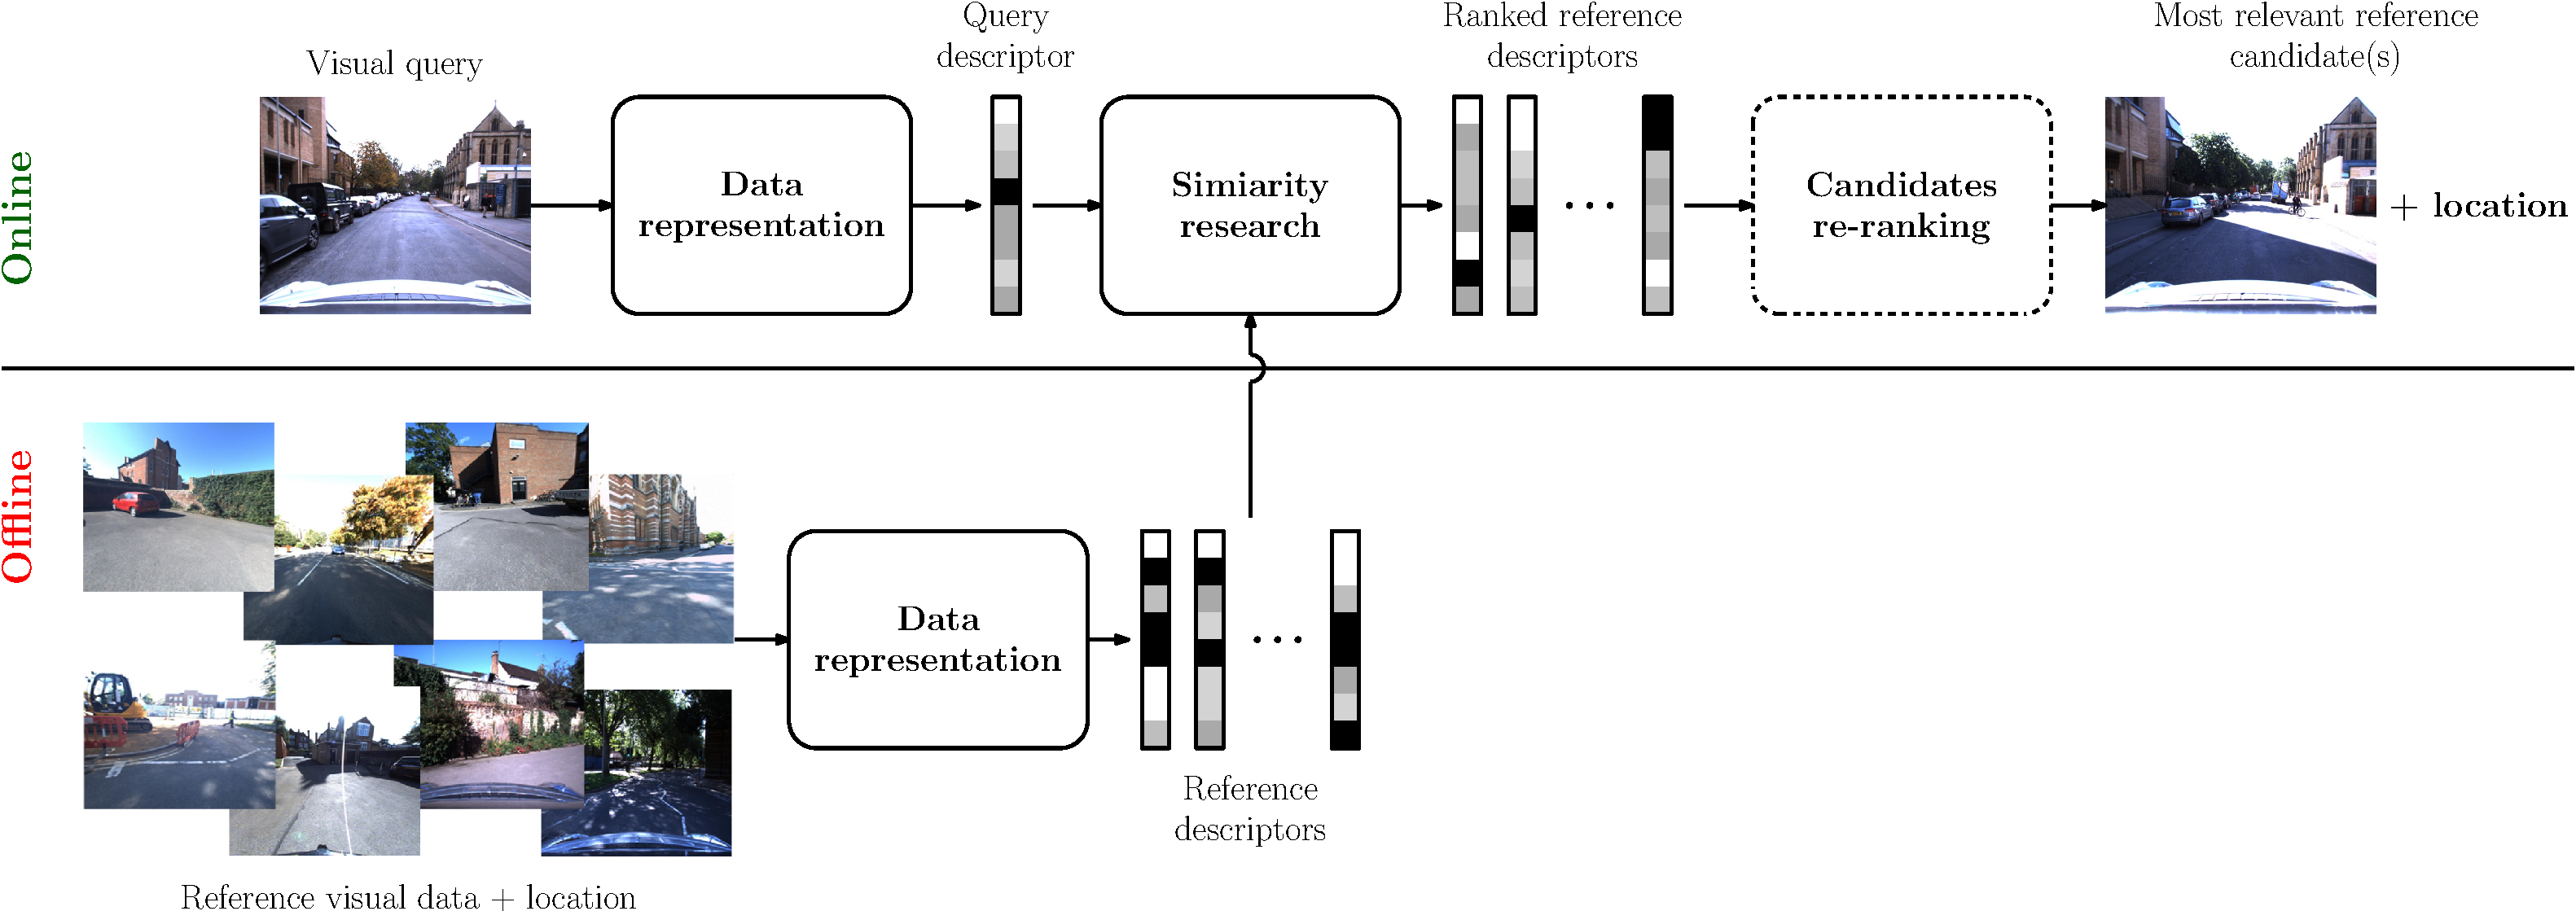
\includegraphics[width=\linewidth]{methods/cbir_for_localization}
	\caption[CBIR for localization]{\label{fig:cbir_for_localization}\textbf{CBIR for localization:} the location of a given request can be retrieved by comparing the query to a pool of geolocalized candidates. After the similarity comparison, the location associated to the top-ranked reference data is considered as the location of the query. Re-ranking of the reference data can be used in order to improve the relevance of the top-ranked candidates.}
\end{figure}


\label{subsec:vbl_as_image_retrieval}
The aim of \ac{cbir} methods is to retrieve a set of data presents in the database that are similar to an input query. This is a problem related to instance retrieval~\citep{Zheng2017}. As the visual data used in \ac{vbl} are augmented with geospatial information (\textit{e.g.} a geotag associated to an image), retrieving documents comparable to the input provides an information on the possible location of the query. This localization method is three-step: description of the visual data, similarity association across the description vectors previously extracted and possible candidates re-ranking. \acs*{cbir} for localization pipeline is illustrate in figure~\ref{fig:cbir_for_localization}.

\subsubsection{Efficient data representation for localization}
As one of our main contribution in this thesis targets the design of a new learned global image representation for long-term \ac{cbir} for localization, we do not detail data description in this chapter. We refer reader to the first section of \acl{chp}~\ref{chap:3}, \acs{sec}~\ref{sec:cbir_data_for_loc}, for a comprehensive review of image representation suited for localization.

For the subsequent tasks of the localization process, we assume that we are able to produce low dimensional vectors to describe the visual data.

\subsubsection{Similarity Research}
\label{subsubsec:similarity_research}

The similarity research step involve evaluating the sameness between the request descriptor (\ie the description vector computed from the visual request we want to localize) and the reference descriptors. At the end of this step, we obtain a list of reference candidates, ranked accordingly to their similarity to the request.

\paragraph{Pre-processing.}
Dimension reduction of descriptor is often performed to reduce matching time and memory footprint. The most used technique remains the \ac{pca}. \ac{pca} is applied on hight dimension vector, \textit{e.g.} weights extracted from CNN layers (\citep{Arandjelovic2017,Gordo2016}). \ac{pca} has also been used to reduce the size of local features aggregated vectors \citep{Kim2015,Torii2015} or global descriptors \citep{Ni2009}. Gaussian Random Projection is applied in~\citep{Sunderhauf2015a,Panphattarasap2016} and in a different work, binary locality-sensitive hashing~\citep{Sunderhauf2015} is used instead. To reinforce data consistency, whitening could be applied to final features before the similarity search~\citep{Jegou2012a,Gong2014,Tolias2016,Arandjelovic2017,Gordo2016,Radenovic2016}.

\paragraph{Similarity metric.}
For most methods, comparison between descriptors is a trivial operation: it consists in a simple euclidean distance computation between vectors (with $L2$ norm or cosine similarity -- \textit{if the vectors are unitary} -- as usually used metric). Area correlation is another approach for computing data similarity. Simple forms of correlation like Sum of Squared Difference (SSD) or Sum of Absolute Difference (SAD) have been used in \ac{vbl} to directly compare raw images~\citep{Poglitsch2015,Milford2015}. \citet{Wan2016} use PC (Phase Correlation) on images described with FT (Fourier Transform) in order to be robust to shadow artifacts. In the work of~\citep{Corke2013}, authors compare shadow invariant grey-scale images with Zero Mean Normalized Cross-Correlation (ZNCC).

\paragraph{\Acl{nn} Search.}
In some works, when the amount of data to compare remain acceptable, linear or brute-force retrieval procedure can be employed to retrieve the closest neighbors. Hierarchical structures can be used in order to speed-up the research process (\eg k-d-tree). Linear \ac{nn} search is used in~\citep{Babenko2014,Sunderhauf2015,Radenovic2016,Gordo2016,Arandjelovic2017,Zamir2010,Zamir2014,Sunderhauf2015a}, among others, where low-dimension global image descriptor (\S\ref{subsec:global_feature}) are used to describe the data.

Exact nearest neighbor search becomes impracticable when the amount and/or dimensionality of the features are too large. Authors then turn to approximate nearest neighbor search to trade efficiency for rapidity, thus accepting some errors in the retrieved neighbors. Approximate matching involve hashing methods~\citep{Gionis1999}, well-suited data structure like inverted-index and quantization frameworks~\citep{Nister2006,Philbin2007,Jegou2011}. Interested readers may see~\citep{Wang2017} for more details.

Several \ac{nn} search algorithms are efficiently implemented in the \texttt{FLANN} library~\citep{Muja2009}, and in the new Facebook \texttt{FAISS} library~\citep{Johnson2017}.

\paragraph{Machine Learning matching Methods.}
Learning the distribution of the extracted features is an alternative to aforementioned \ac{nn} search methods.

\Ac{svm} classifier is used in numerous works~\citep{Shrivastava2011,Cao2013,McManus2014,Aubry2014} to cast the similarity research as a classification task. \citet{Cao2013} initially cluster the database according to the resemblance of the images. On top of this graph of similar images, they trained \ac{svm} for each cluster and at query time oppose the input image to all classifiers. By selecting the data associated to the \ac{svm} reaching the higher score of classification, this approach permits to quickly retrieve a pool of similar images. In~\citep{McManus2014,Aubry2014} authors train linear classifiers on HOG descriptors to robustly retrieve similar images that present extreme appearances changes. \citet{Aubry2014} take the advantages of \ac{lda} data representation in order to avoid expensive \ac{svm} training (like hard negative mining used in~\citep{Shrivastava2011,Kim2015}). Similarly, \citet{Kim2015} train \ac{svm} classifier to predict the robustness of extracted descriptors. This improves the matching process and reduces the number of features to compare against the database.

\citet{Lu2015} introduce a \ac{mtl} layout designed for features similarity association. Works from \citet{torralba2003context} and \citet{Ni2009} present \ac{vbl} methods that are able to localize an input query among a set of predefined places. Authors embedded the recognition process into probabilistic framework, \ac{gmm} in~\citep{torralba2003context} and epitome in~\citep{Ni2009}, trained upon images representing different areas. Such paradigms allow an easy integration of additional features (such as depth information~\citep{Ni2009}).

\paragraph{Other Matching Methods.}
\citet{Stumm2015a} introduce an innovative method based on graph matching. The visual vocabulary abstraction is employed and augmented with a graph of covisibility of the visual words in images. The graph is constructed as follows: nodes represent visual word detected in images and edges are created between two nodes if they are seen together in a same image. This formulation permits integrating geometric relations between the extracted features. Authors use a graph kernel for the similarity comparison among the query graph and the database~\citep{Stumm2015,Stumm2016}. Notice that graph-based approaches are often employed when scenes are described by spatially organized semantic clues such as office furnitures~\citep{Salas-Moreno2013} or street equipments~\citep{Ardeshir2014}.

\subsubsection{Candidates re-ranking}
\label{subsec:candidates_re_ranking}
Data can be processed after the similarity research to improve the final result. Post-processing methods are widely used to re-rank the candidate list, improving relevance of retrieved data.

\paragraph{Generic re-ranking.}
Query expansion is a post-process that re-query the database after a first retrieval step to increase the recall rate~\citep{Chum2007,Chum2011,Tolias2014}. However, increasing the recall rate is not the main concern of \ac{vbl} indirect method~\citep{Sattler2012}. Indeed, as exposed in the introduction, a perfect \ac{vbl} indirect system should retrieve at first position the closest visual document present in the database. However, more suitable top ranked candidates in the list of retrieved data could benefit to a subsequent pose estimation step~\citep{Song2016}. The \ac{vbl} system presented by \citet{Cao2013} increase the diversity of retrieved images by introducing a probabilistic re-ranking on the assumption that the first ranked candidate is not a good one and by maximizing the probability that the second one is.
\label{par:ransac}
On the other hand, geometric consistency check is often used to reject wrong matching. Relative pose between the query and the database candidates is computed by considering homography or multiple-view transformation, and candidates that produce the most consistent pose are ranked up. \citet{Philbin2007} democratize the use of spatial verification by introducing prior on the pose of the photography by assuming a top-oriented view. Authors perform spatial check hierarchically to get more flexibility between time computation and retrieval precision. The geometric transformation between the query and the candidate is usually computed with minimal algorithm embedded in random consensus, like RANSAC~\citep{Fischler1981}. There exists multiple alternatives to the classical RANSAC algorithm. PROSAC by~\citep{Chum2005}, used in~\citep{Donoser2014}, prioritize specific features during the random selection step. We can also enumerate LO-RANSAC used in~\citep{Philbin2007} and AC-RANSAC in~\citep{Qu2015,Qu2016}. Novel method F-SORT presented by \citet{Chan2016} show outstanding result both in term on matching quality and computation efficiency. Notice that these algorithms, beside improving the relevance of the retrieved candidates, can give information about the relative pose of the query. That is why numerous 6 \ac{dof} pose estimation methods, presented thereafter in \acs{sec}~\ref{subsec:fine_pose_estimation}, rely also on these techniques.

\paragraph{Specific \ac{vbl} re-ranking.}
Unlike conventional methods of object-retrieval, indirect \ac{vbl} can benefit from geo-localization information associated to the documents present in the database. As discussed earlier, this information can be used to construct structured graph for the similarity search process~\citep{Torii2011,Cao2013} or exploited to re-rank the candidates list~\citep{Zamir2010,Zamir2014,Sattler2016}. \citet{Zamir2010} introduce this geographic re-ranking after a classical image-retrieval algorithm to quickly remove irrelevant candidates. Authors go one step further in~\citep{Zamir2014} and embed the matching process within a Generalized Minimum Clique Graphs scheme to retrieve consistent candidates according to the GPS tag associated to the visual data. \citet{Sattler2016} generalize the problem of visual burstiness introduced by~\citep{Jegou2009} to a geographic level, introducing the concept of geometric burstiness. They improve the relevance of the ranked list of candidates using position and popularity meta-information of database images.

\subsection{6 \acs*{dof} pose estimation}
\label{subsec:fine_pose_estimation}

At this point, we introduce camera pose estimation methods that instantly recover the exact 6 \ac{dof} pose of the query according to a known reference. Compared to \ac{cbir} approaches, 6 \ac{dof} pose estimation methods provide a more accurate query pose to the detriment of the area coverage. From this class of methods, we consider the two following approaches:
\begin{description}
	\item[Geometric methods:] this class of methods, also known as structure-based methods, performs the global localization of the query by establishing correspondences between two-dimensional features extracted from a visual query and three-dimensional model of the environment (see figure~\ref{fig:geometric_method}).
	\item[Learned approaches:] the last considered family of algorithms are methods that learn to directly regress from an input visual data to its corresponding pose. Standard regression techniques~\citep{Shotton2013} and \ac{cnn} architecture~\citep{Kendall2015} are employed to perform this task (see figure~\ref{fig:learned_method}).
\end{description}


\subsubsection{Geometric methods}
\begin{figure}[t]
	\centering

	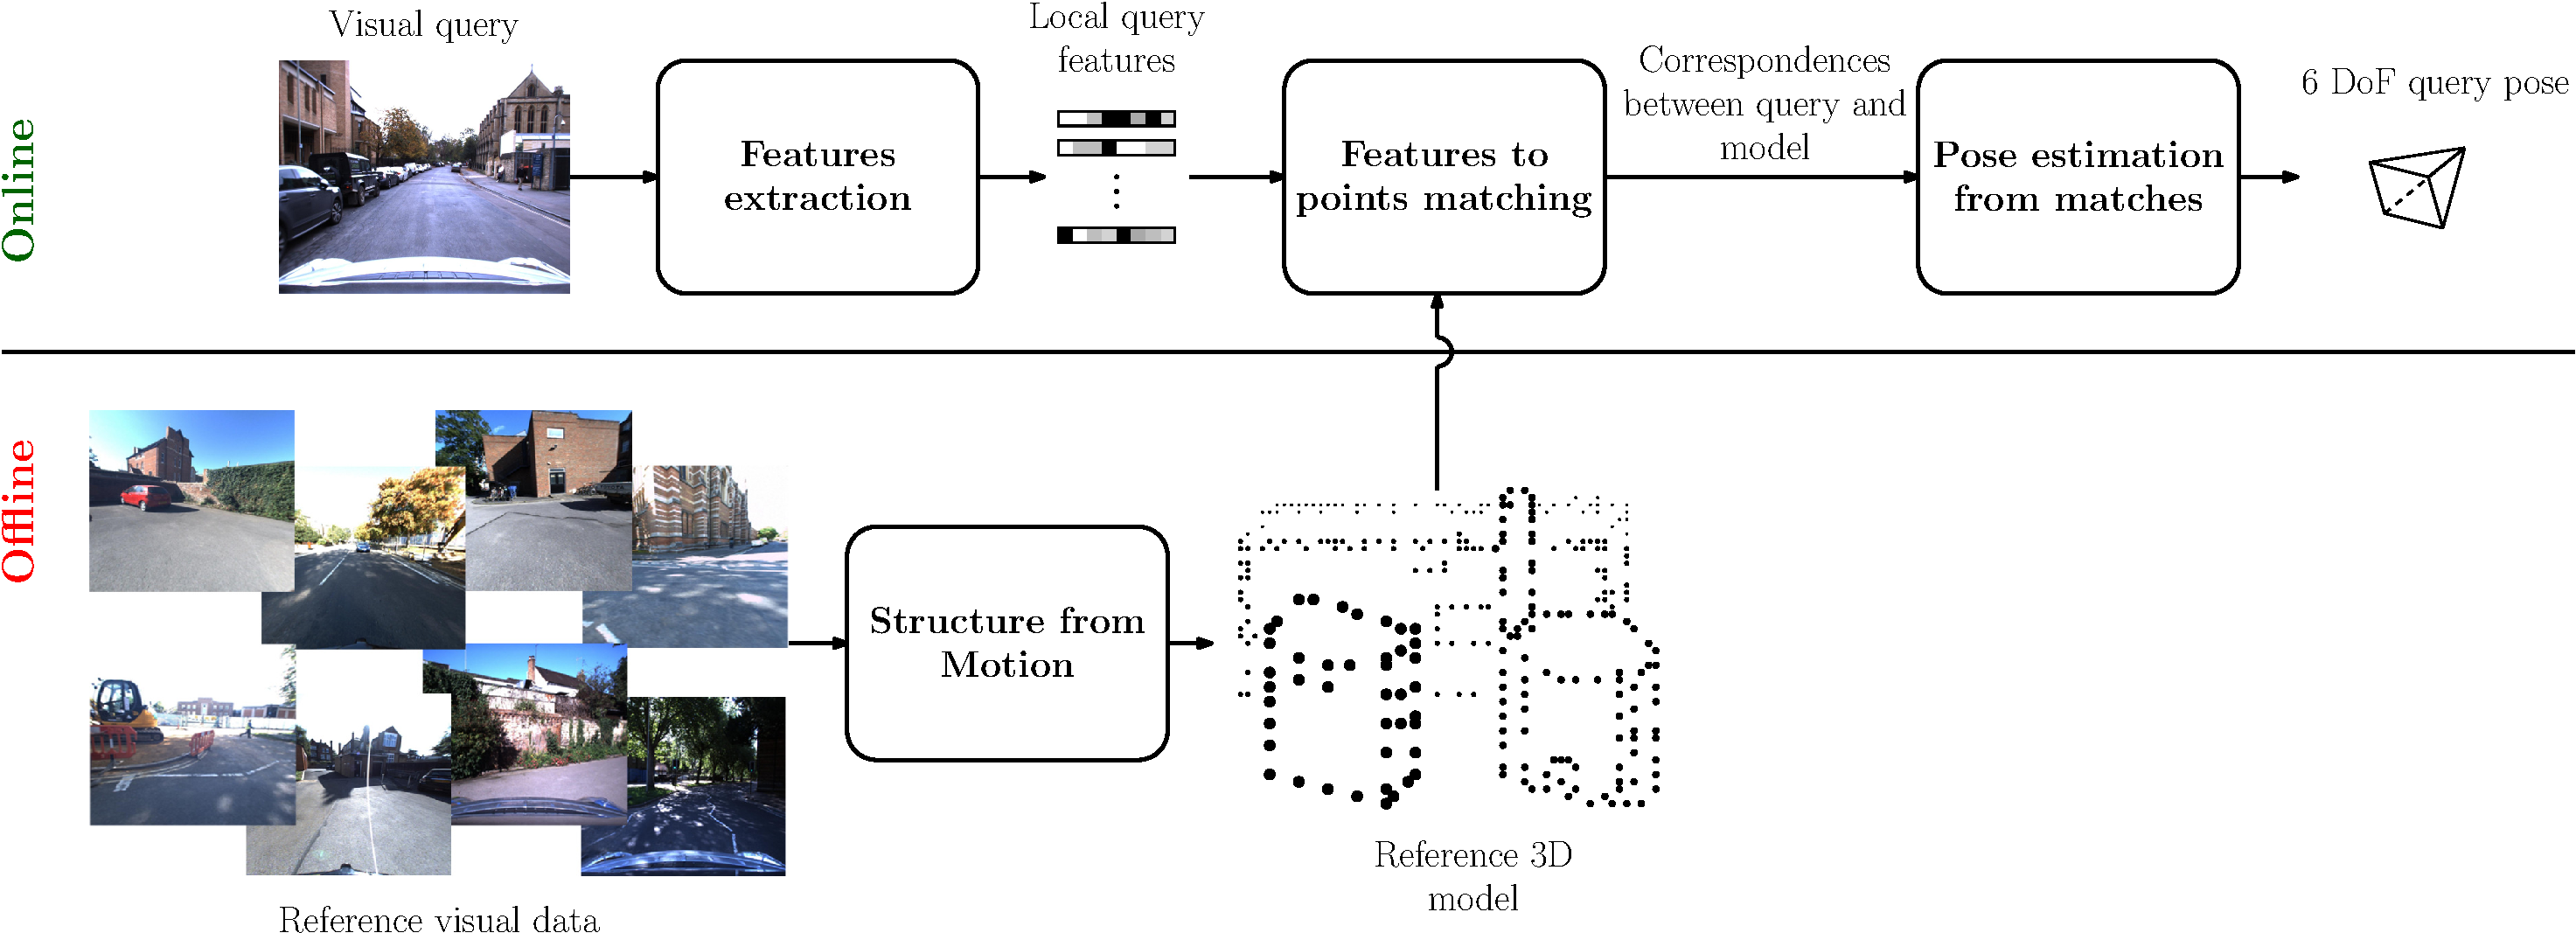
\includegraphics[width=\linewidth]{methods/geometric_method}
	\caption[Structud-based method]{\label{fig:geometric_method}\textbf{Structure-based \acs{vbl}:} reference data are used to construct a 3D model of the environment. During localization, the query is compared to this model to determine its 6-\ac{dof} pose.}
\end{figure}


\label{subsubsec:sfm_methods}
A widely represented family of \ac{vbl} methods aims to regress the pose of a camera based on the analysis of a 3D point cloud reconstructed by \ac{sfm} algorithms~\citep{schoenberger2016sfm,moulon2016openmvg,rupnik2017micmac}. The principle of these methods is to establish 2D features to 3D points correspondences (F2P). In a first step, three-dimensional representation of the environment is built thanks to many images. Triangulated points within this structure are associated to the local features (most of the time SIFT vectors~\citep{Lowe2004}) extracted from all the images where the considered point is visible. At query time, local features from the image to localize are matched against the set of pre-computed 3D points. Finally, the features to points correspondences permit a 6 \ac{dof} pose estimation of the acquisition system. The overall pipeline of structured methods is presented in figure~\ref{fig:geometric_method}.

These methods have a lot in common with \ac{cbir} for localization approaches described in Section~\ref{subsec:vbl_as_image_retrieval} as they share two major steps:~feature extraction and data association. Yet, the use of a geometrically structured database introduces interesting elements not exploitable in a classical image-retrieval scheme~\citep{Sattler2012a}.

\paragraph{Features to points matching.}
As \ac{nn} search have already been presented in the previous section\ref{subsubsec:similarity_research}, in this paragraph we focus on more specific matching methods designed for geometric \ac{vbl}.

\citet{Irschara2009} introduce the first F2P method based on \ac{sfm} environment representation. Authors perform scalable \ac{vbl} by registering the point cloud into synthetic visual documents covering the entire model. Latter improvement by \citet{Li2010} reverse the conventional process by searching from the point cloud correspondences in the image (P2F), instead of matching features from the image to points. This formulation causes an overhead in computation but is correctly handled by considering a compressed version of the \ac{sfm} model and by implementing end-conditions and rejection cases in their algorithm.

\citet{Sattler2011} consider the original features to points correspondences scheme by~\citep{Irschara2009} and introduce a Vocabulary-based Prioritized Search (VPS) inspired by BoF matching method. Subsequent works by the same authors~\citep{Sattler2012} augment the VPS framework with the points to features matching P2F~\citep{Li2010}. \citet{Li2012} show that the class of methods introduced in~\citep{Irschara2009,Li2010} can deal with large environment. Authors augment the P2F matching with hypothesis of co-occurrence of 3D points present in a close neighborhood. Based on similar spatial observation, \citet{Sattler2015} consider visibility graph to reject wrong matchings. \citet{Heisterklaus2014} introduce MPEG compression for visual document in order to speed-up the system. In the work described in~\citep{Donoser2014}, authors use the descriptor redundancy associated to 3D points to train random ferns on the top of each points. F2P matching time requirement is by the fact greatly reduced. 

Works from~\citep{Middelberg2014,Lynen2015} tackle the problem of \ac{vbl} embedded in a mobile device with limited memory storage and computational power. To achieve real-time performances, authors in~\citep{Middelberg2014} produce a very light 3D model to track the mobile camera in an urban environment. They send at regular interval key-frames to a server that is in charge of computing the global pose of the camera regarding a pre-produced point cloud. Aligning a light relative point cloud reconstructed with \ac{sfm} to a bigger one have also been investigated in~\citep{Lu2015}. \citet{Svarm2014} consider the problem of \ac{vbl} with F2P matching as a combinatorial optimization problem and design a fast outliers rejection scheme. This promising work have been improved through~\citep{Zeisl2015,Svarm2016} contributions.

State of the art strucutred methods based are dominated by techniques combining previously mentioned improvements~\citep{Sattler2016a}. Recent work by \citet{Feng2016a} reduce drastically the computational power requirement by considering fast point extractor and binary descriptors combined with an efficient similarity research. Authors show an order of magnitude in time reduction without any pose estimation performances deterioration.

\paragraph{Pose estimation.}
\label{para:pose_estimation}
F2P (as well as P2D) provides correspondences between 2D pixels and 3D points. Defined by \citet{Hartley2003}, perspective-$n$-point (P$n$P) formulation is the most common tool to recover the absolute camera pose according to a point cloud reconstructed by \ac{sfm}.

Embedded in a random consensus scheme (see \S\ref{par:ransac}), six correspondences between the image and the 3D model are sufficient to retrieve the pose, if we have no information about the intrinsic parameters of the camera~\citep{Donoser2014,Li2010,Li2010,Heisterklaus2014}. This formulation is known as P6P and can be solved with Direct Linear Transformation (DLT \citep{Hartley2003}).

In particular cases, three correspondences between the image and the model are sufficient (P3P pose computation problem). Especially, the pose estimation problem can be reduced to a P3P formulation if the intrinsic parameters of the camera are known~\citep{Irschara2009,Middelberg2014}, or if 3 or more \ac{dof} are fixed~\citep{Zeisl2015,Qu2016,Svarm2016,Svarm2014}. In those particular cases, P3P solvers~\citet{Kneip2014opengv} are mostly used to recover the pose.

\subsubsection{Learned methods}
\begin{figure}[t]
	\centering

	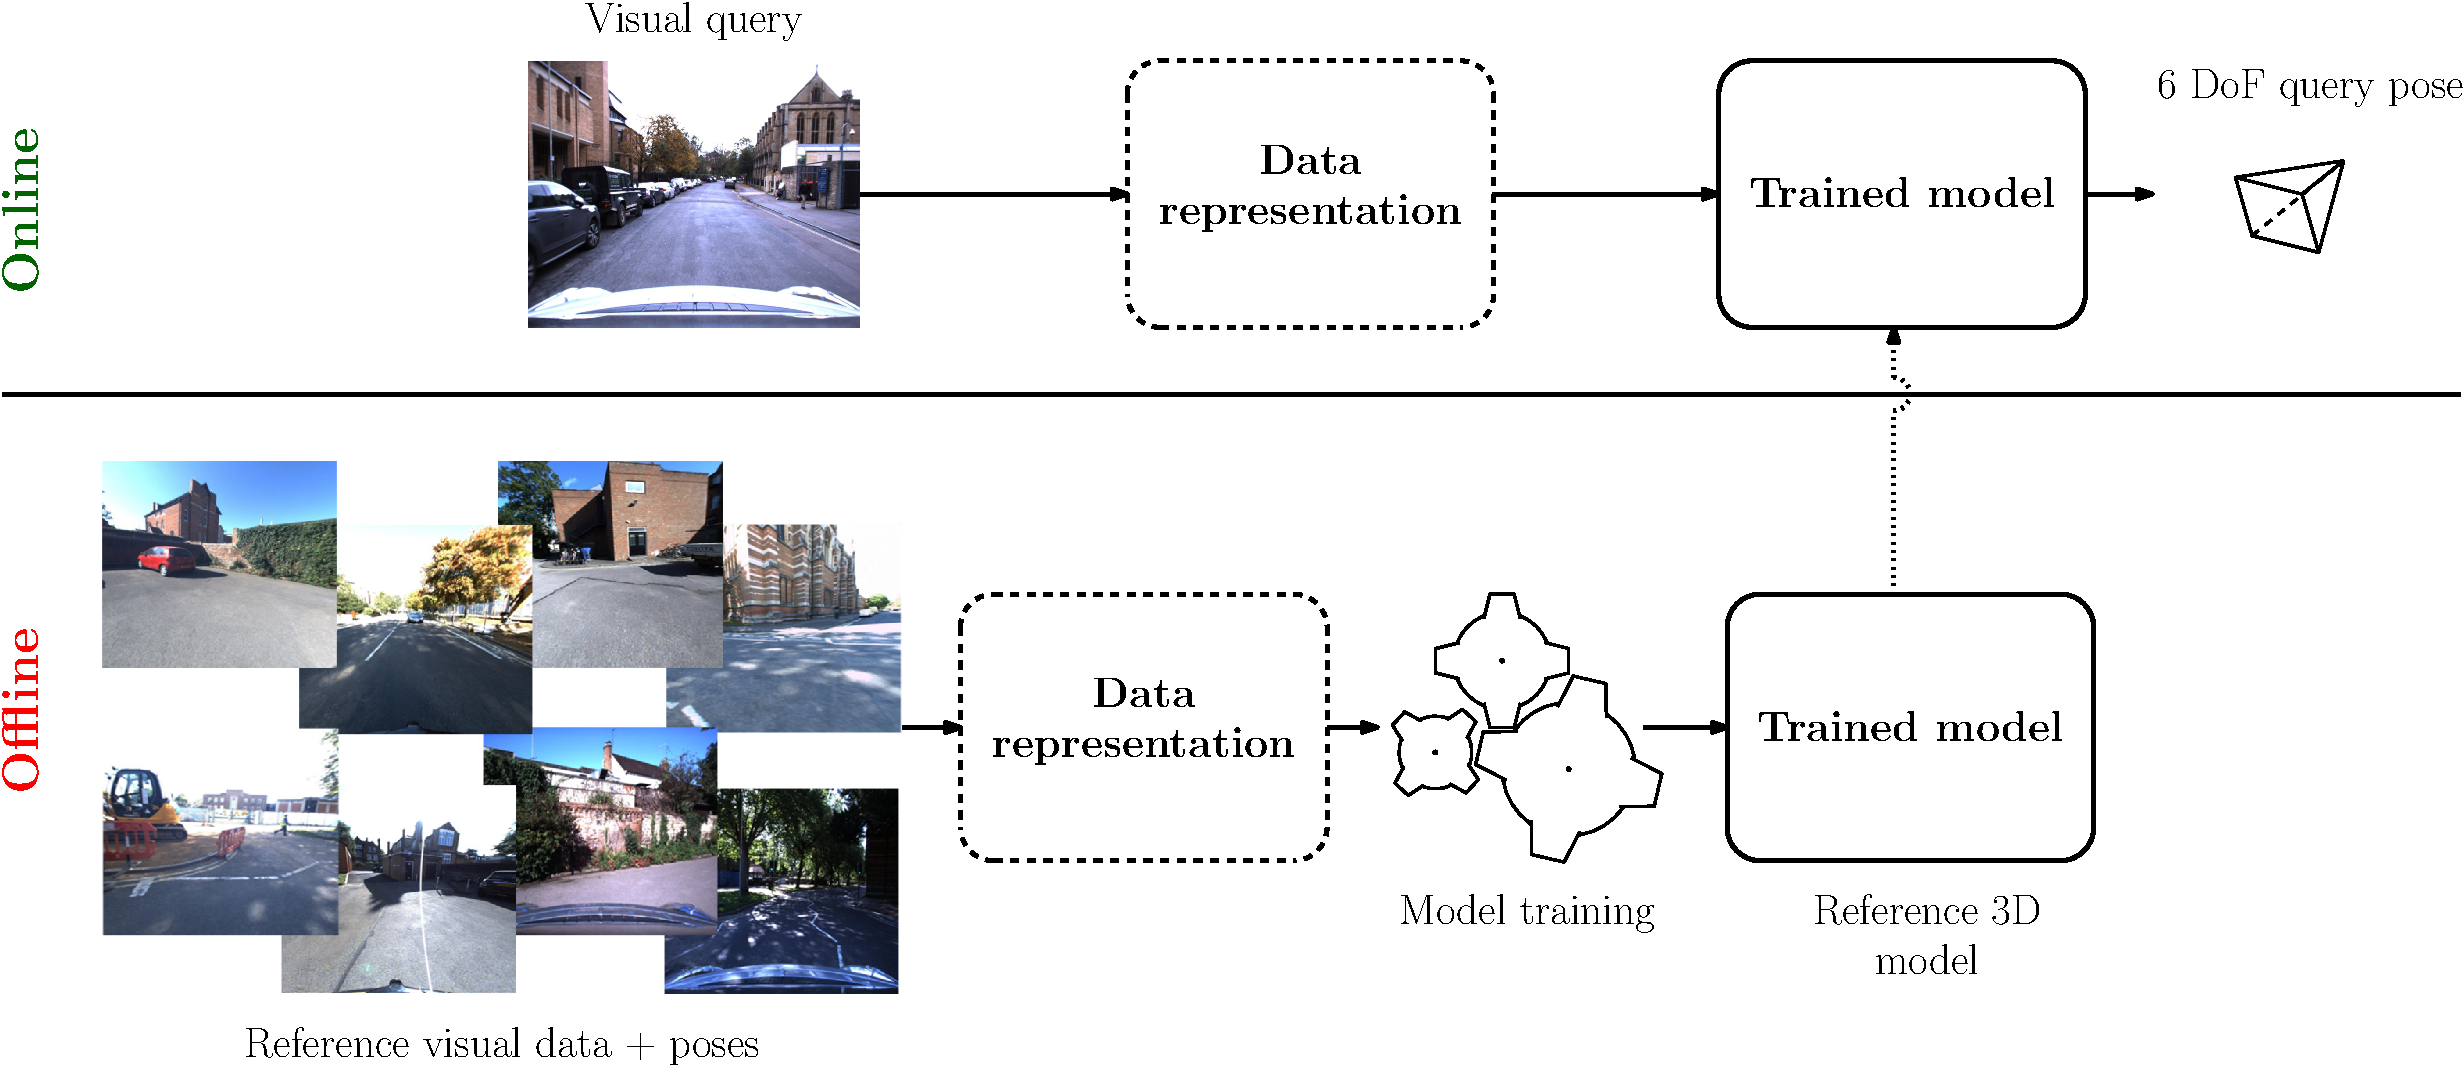
\includegraphics[width=\linewidth]{methods/learned_method}
	\caption[Learned method]{\label{fig:learned_method}\textbf{Learned method for \acs{vbl}:} a model is trained with geolocalized data in order to regress the right pose of a visual request. Once trained, the model is used to predict the pose of a unknown query. The data can be preprocessed before the evaluation by the model.}
\end{figure}


\label{subsubsec:pose_regression}
The last class of 6-\ac{dof} pose estimation methods cast \ac{vbl} as a machine learning problem. A model is trained with geolocalized visual data in order to be able to predict the 6-\ac{dof} pose of an unknown visual request. Key components of learned methods are presented in figure~\ref{fig:learned_method}. If the scene geometry is totally known, local method can be applied~\citep{Shotton2013} (\ie the data involved in the learning processes are local feature or raw pixels). Otherwise, the method is global and entire images are used as input to the model~\citep{Kendall2015}.

\paragraph{Local methods}
\begin{figure}
	\begin{minipage}{0.58\linewidth}
		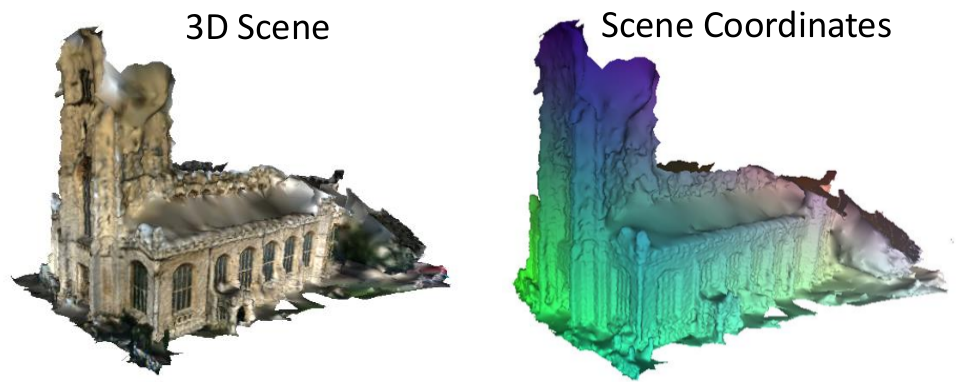
\includegraphics[width=\linewidth]{methods/scene_coordinates}
	\end{minipage}
	\begin{minipage}{0.4\linewidth}
		\caption[Scene coordinates repesentation]{\label{fig:scene_coordinates}\textbf{Scene coordinates repesentation:} local learned-based \acs{vbl} method rely on scene coordinates representation of the environment to retrieve the 6-\acs{dof} pose of a query. Model on the right is colorized according to the $xyz$ position of the 3D points mapped in RGB color space. Figure from~\citep{Brachmann2017b}.}
	\end{minipage}
\end{figure}

First introduced by~\citet{Shotton2013}, local learned method for \ac{vbl} are based on the scene coordinates representation of the environment. Scene coordinates representation associates to each pixel of an image its 3-dimension coordinate in a global scene frame. It means that we requires both image 6-\ac{dof} pose as well as scene geometry (\eg depth map associated to the image) to create a scene coordinates representation. See figure~\ref{fig:scene_coordinates} for a colorized example of scene coordinates representation. During training, we minimize the error between predicted 3D coordinates of each pixel of a training set of images with the ground truth scene coordinates. Once the model is trained, we can use it to predict dense 3D coordinates at each pixel position of a new image. Finally, these 2D-3D correspondences (2D position of pixels' image and predicted 3D coordinates) are used to compute the 6-\ac{dof} of the query image. Similar algorithm as the ones used for structure-based methods (see section~\ref{para:pose_estimation}), embedded in a random consensus, are used in order to compute the query pose. This class of method is compact but not scalable: it requires to train one model by scene.

In the initial works by~\citet{Shotton2013}, authors use a regression forest to learn the mapping from pixel to 3D scene coordinates. At query time, a handful of pixels from a depth camera frame are processed into the regression forest. This method is fast and precise and can be used on texture-less data. However, the depth information associated to each pixel is needed at test time. This initial method have been improved in~\citep{Guzman-rivera2014}, where authors take in consideration several candidates for the final pose regression obtained by multiple trained predictors. \citet{Valentin2015} introduce mixture of Gaussian to represent the uncertainty associated with the regression forest prediction and significantly improve the 6 \ac{dof} estimation by embedding this information within the full camera pose regression step. The regression forest have been replaced by Neural Network (NN) in~\citep{Massiceti2016}, bringing slightly better result at the cost of computational overhead. \citet{Meng2016} consider only RGB images at query time. The loss in precision is compensated by a post pose refinement step based on nearest neighbors search with sparse extracted SIFT features (like in structured approaches, see section~\ref{subsubsec:sfm_methods}).

\citet{Duong2018} introduce a patch-based approaches where area centered on keypoints extracted from standard image detector are used instead of raw pixels. During training, they use a \ac{cnn} to predict 3D-coordinate from the extracted image patches. In major work of~\citet{Brachmann2017b}, the complete image is used as input to a fully-\ac{cnn}. The model predict a dense scene coordinates image and the authors perform end-to-end training regarding the final pose prediction thanks to a differentiable version of RANSAC (DSAC~\citep{Brachmann2017}). They obtain convening results using only images and they show that their method can be applied even if we do not know the full geometry of the scene. In~\citep{Li2018}, a new loss function is introduced to stabilize the training of fully-\ac{cnn} for dense scene coordinates prediction.

To address the scene-dependent limitation of classical methods, \citet{Glocker2015} design a system based on regression ferns to quickly associate an RGB-D image to a binary feature. Ferns produce descriptor according to randomly initialized binary rules, and a look up table is maintained to directly associated image signature with 3D pose in the scene. Presented system is less precise that the one presented by~\citet{Shotton2013} but has the advantages of not relying on a heavy pre-processing step (\ie the spawning of the regression forest). Along the same line, promising work of \citet{Cavallari, Cavallari2018} propose to quickly adapt a pre-trained regression forest to a new scene. This method permit to recover the pose of a RGB-D camera frame, more precisely than~\citet{Glocker2013,Glocker2015}, without the costly step of complete regression forest training. Recent work in~\citep{Cavallari2019} applied a variant of the precedent method with fully-\ac{cnn} architecture of~\citep{Brachmann2017b} instead of regression forest. They fill coordinates reservoir at the end of a pretrained model with information about a new scene to quickly obtain a precise localization system.

\paragraph{Global methods}
\label{para:cnn_regressor}
Introduced in 2015 by \citet{Kendall2015}, the first global learned method, PoseNet, consists of a fine-tuned \ac{cnn} for the task of 6-\ac{dof} pose regression. The network is trained upon a set of paired image/pose and directly regress the 6-\ac{dof} pose of a camera from an image. The pose obtained through this method is not as accurate as the pose obtained with geometric or local method~\citep{Feng2016a,Brachmann2017b} but provides great tolerance to changes in scale and appearance. Compared to scene coordinates-based methods~\citep{Shotton2013,Li2018}, \ac{cnn} seems more appropriate to handle large environment and does not rely on depth information.

Recent improvement have been proposed by the original authors~\citep{Kendall2016} to integrate an uncertainty estimation in the regression process. \citet{Liu2016} consider this \ac{cnn} architecture with only depth map information, acquirement with active depth sensor, for recovering the pose of a camera in complete obscurity. The work by \citet{Walch2016a} present a combination of a PoseNet~\citep{Kendall2015} with a \ac{lstm} units plugged at the output of the network in order to encode stronger spatial information from the image. This combination slightly improves the precision of the system. Authors of ~\citep{Jia2016} propose a new method to gather supplementary image/pose pairs for the network training. They generate artificial images from a dense point cloud model obtained by \ac{sfm} thanks to a rendering software. Computer graphics shaders effects are added on some rendered views for simulating various illuminations. In~\citep{Purkait2018}, the view synthesis procedure is extended to real images thank to the known geometry of the scene. \citet{Contreras2017} exploit this \ac{cnn} architecture in order to create a fixed size map that can be improved by adding new trajectories. Authors were able to reduce the original size of the CNN by factor of three while maintaining similar localization performances on indoor scenes. Recent contribution~\citep{Kendall2017} investigate new loss-functions for the training phase of the \ac{cnn}, by adding constraints from multi-view geometry standards~\citep{Hartley2003}. MapNet~\citep{Brahmbhatt2017a} introduces relative constraint between two consecutive images in order to train the regression network with unannotated data. For this training setup, the relative pose between two images is computed by a \ac{vo} algorithm~\citep{engel2017direct,forster2016svo}. In a similar manner, VLocNet~\citep{Valada2018} benefits from relative pose information between consecutive frames by relying on two different networks with shared representation: one for absolute pose regression and the over one for relative pose estimation between two images. In a subsequent work~\citep{Radwan2018,Valada}, authors show how multitask~\citep{kokkinos2017ubernet,Kendall2017a,Zamir2018} learning can improve the pose estimation.

Although Posenet-like method has the advantages of being lightweight and relies on only-images, \citet{Sattler2019} show that performances of such methods are less precise than CBIR-based pose estimation (section~\ref{subsec:vbl_as_image_retrieval}). They demonstrate that learned pose regression method are more likely to average the pose of the training examples~\citep{Torii2013} rather that computing a real pose based on geometric constraints. Another disadvantage of Posenet-like methods rely on the fact that a different model has to be trained for each new scene.

Differently, recent work from~\citet{Weyand2016} consider the localization problem as a classification task. They perform a worldwide training on 126M images categorized into 26k places across the globe. According to a given image a \ac{cnn}, named PlaNet, estimates the most likely location of the query over the split map. Localization of multiples photos taken from a common album can be performed by augmenting the original network with a \ac{lstm} layer. \citet{Vo2017} push further the study of such a neural network and conclude that the features extracted from layers of PlaNet are more discriminative to determine the location of an input image that the CNN classifier itself. By extracting features instead of using a classification algorithm, their contribution is closer to the original \ac{cbir} world-wide localization method IM2GPS~\citep{Hays2008} (see section~\ref{subsec:vbl_as_image_retrieval}). \citet{Seo2018} introduce CPlaNet and use combinatorial partitioning in order to improve fine-grained localization. They use several models trained on different earth partitioning in such way that the final query location can be determine by considering the overlap of each model prediction.

\subsection{Coarse to fine localization}

The last family of \ac{vbl} method we consider here are approaches called ``coarse to fine'' localization. In a word, the localization process is divided in two parts: initial coarse localization (with \ac{cbir} for instance) followed by a 6-\ac{dof} precise and relative pose estimation on the reduced search area. As our second principal contribution in this thesis is a new coarse to fine pose estimation method, we save up the presentation of such methods for chapter~\ref{chap:4}.

\section{Data with Dissimilar Appearances}
\label{sec:changing_environment}	

	\begin{figure}[t]
	\centering
    \begin{minipage}{0.44\linewidth}
    		\centering
   			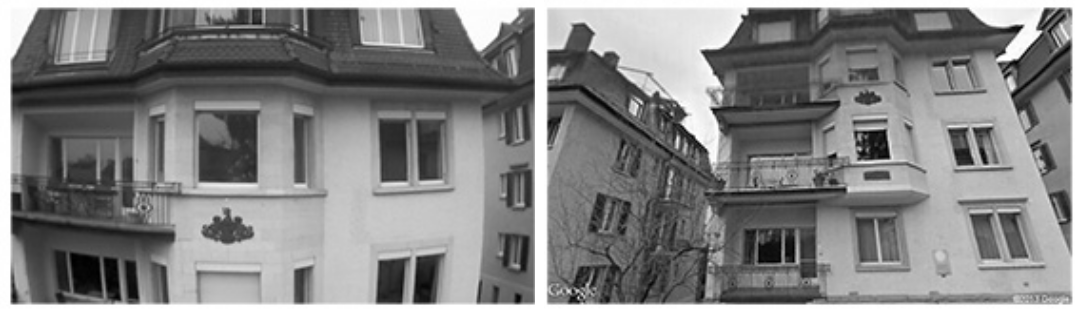
\includegraphics[width=\linewidth]{changes/viewpoint.png}

			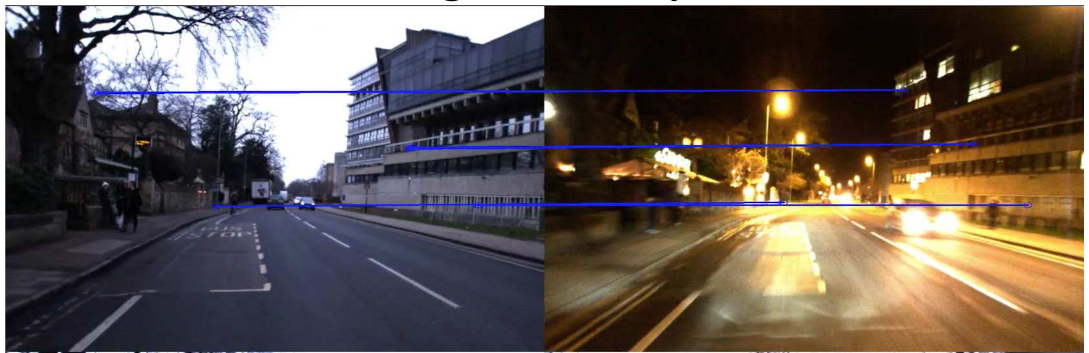
\includegraphics[width=\linewidth]{changes/daynight2.png}
			
			\subfigure[][Appearance changes]{\label{fig:changes}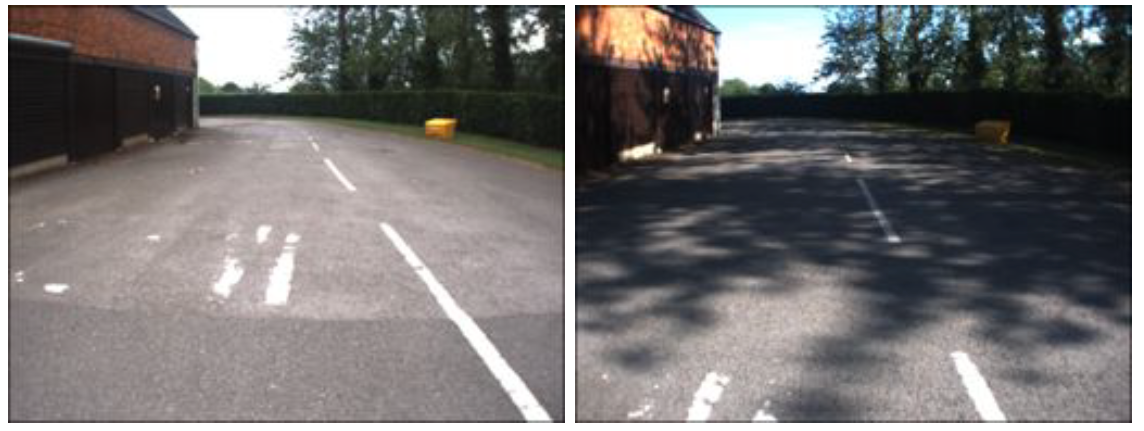
\includegraphics[width=\linewidth]{changes/shadow.png}}
    \end{minipage}
	\hfill
	\begin{minipage}{0.53\linewidth}
   		\subfigure[][Cross-view]{\label{fig:cross-view}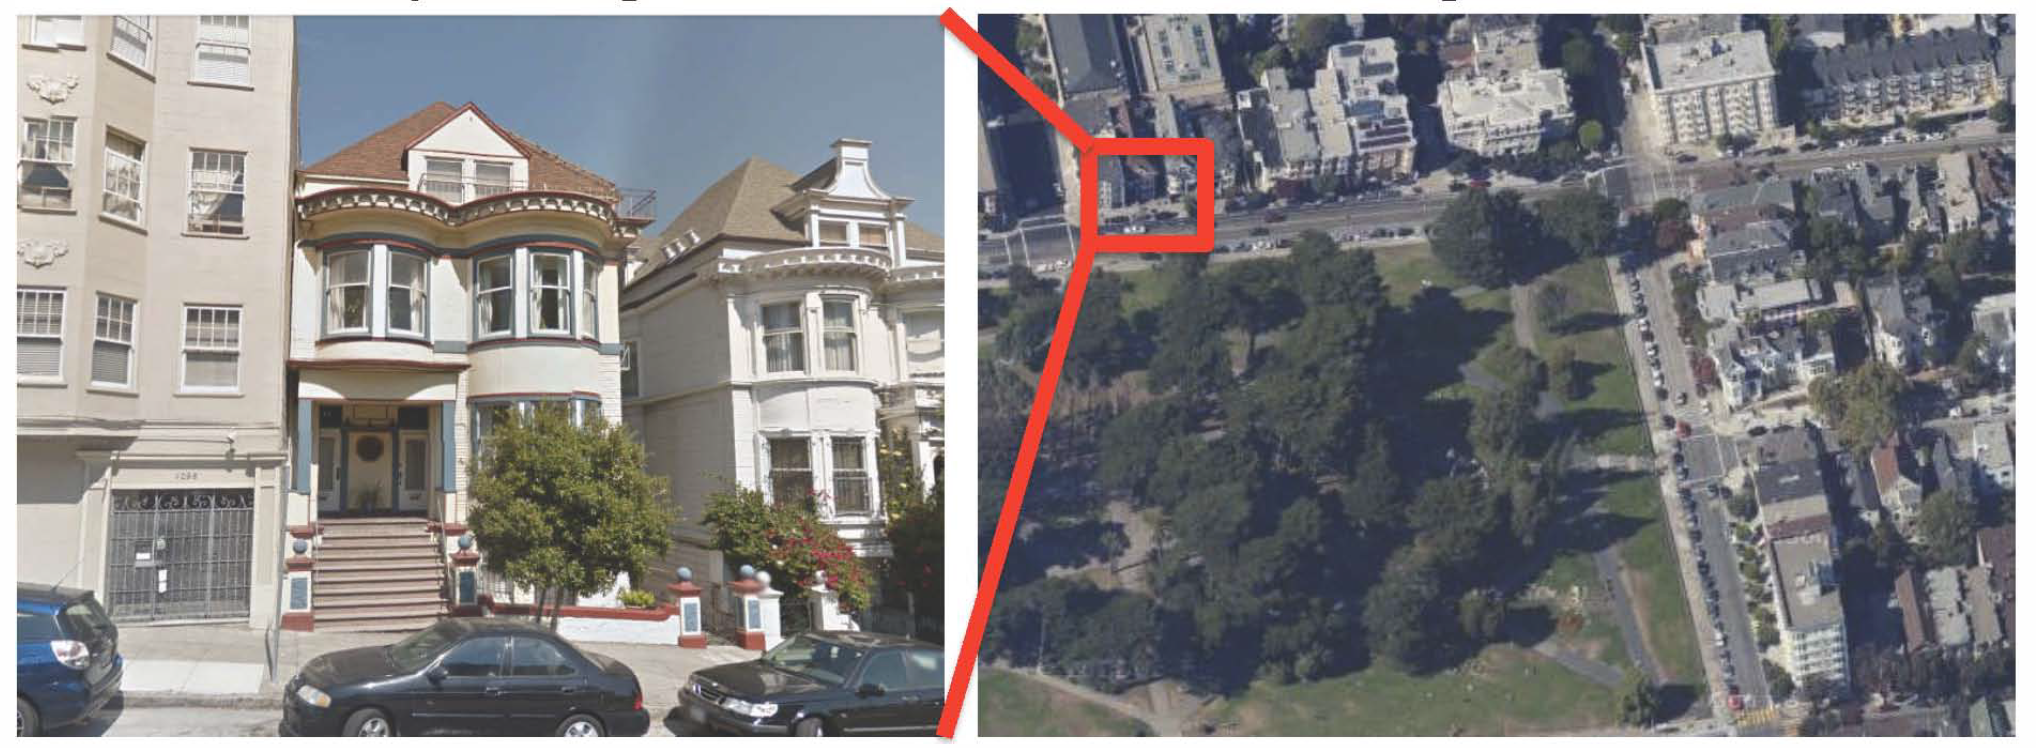
\includegraphics[width=\linewidth]{changes/cross-view.png}}
   		    
   		\subfigure[][Cross-domain]{\label{fig:cross-domain}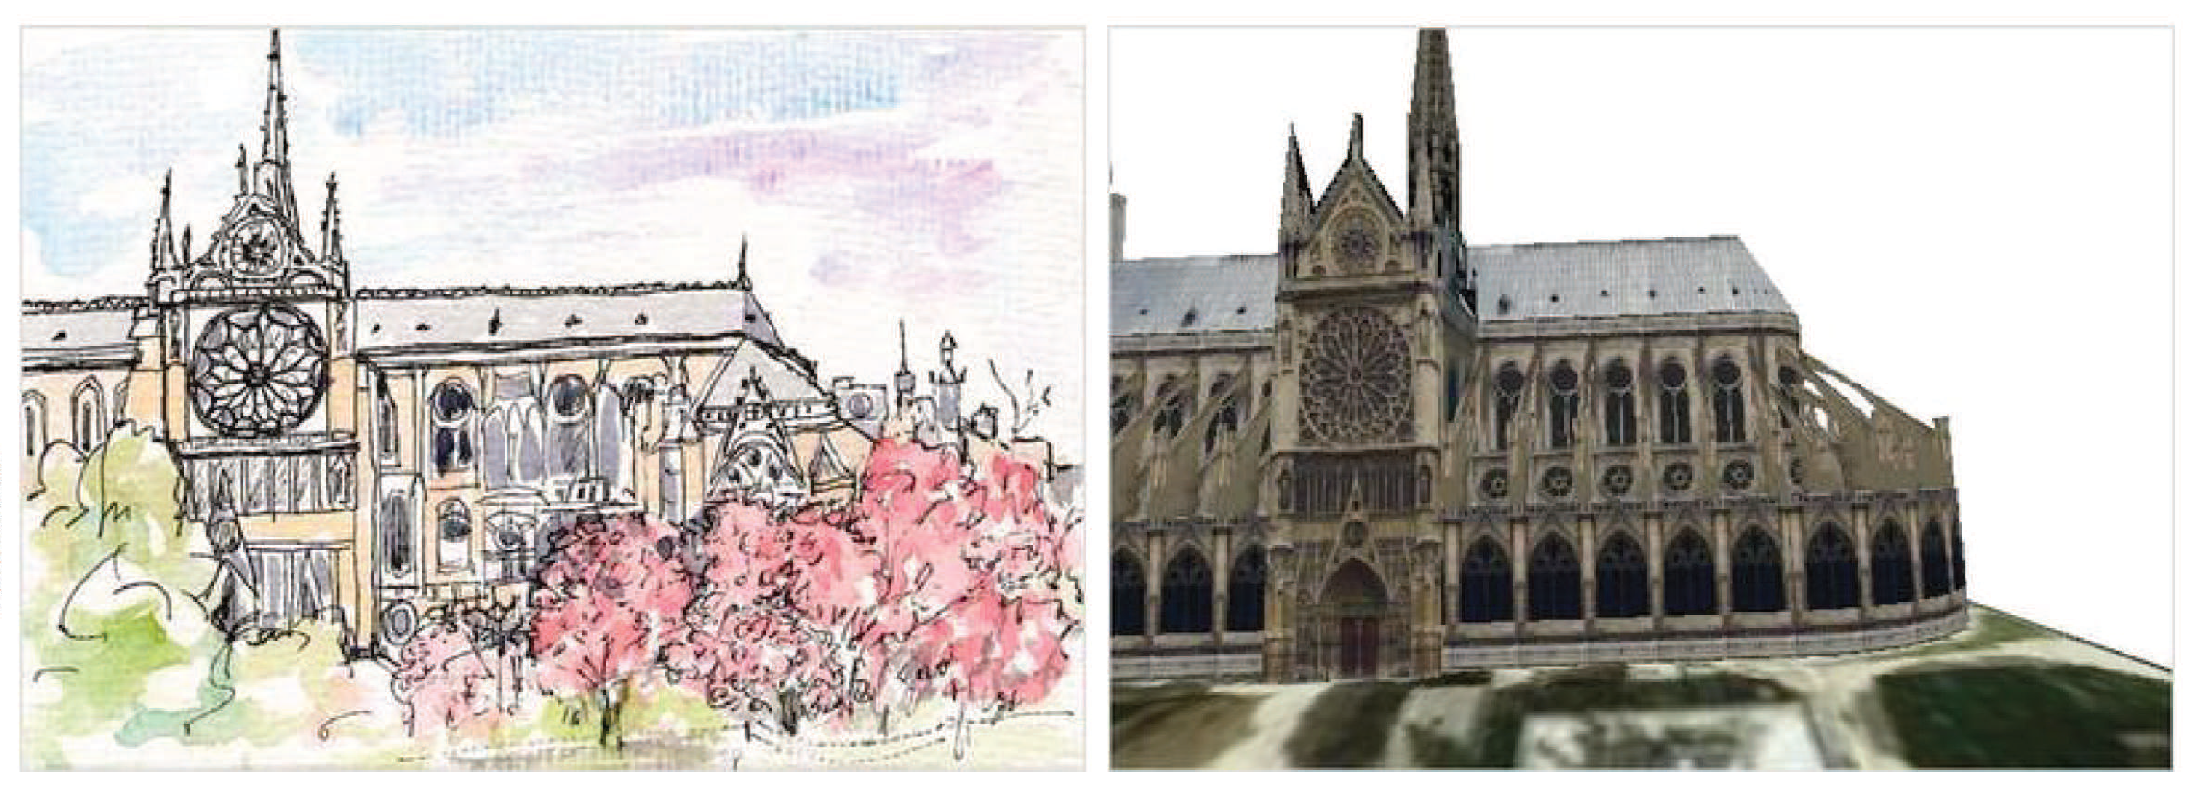
\includegraphics[width=\linewidth]{changes/cross-domain.png}}
	\end{minipage}
	\caption[Illustration of appearance changes present in \acs*{vbl} system]{\textbf{Illustration of appearance changes present in \ac{vbl} system:} \ref{fig:changes}~Visual dissimilarity between the query (left) and the closest image in the database (right). Cause of the change, from top to bottom:~viewpoint differences~\citep{Majdik2013}, daytime to nighttime image matching~\citep{Porav2018} and shadow interferences from~\citep{Corke2013}. \ref{fig:cross-view}~Cross-view localization system~\citep{Lin2015}:~left represent the ground-level query image and right the bird's eye view of the same scene. \ref{fig:cross-domain}~Cross-domain \ac{vbl} system~\citep{Aubry2014}:~on the left the query painting and on the right the corresponding pose according to a 3D model. \label{fig:data_changes}}
\end{figure}


	As pointed out by \citet{Lowry2016}, permanent changes occurring in our environment is a huge concern in vision domain. In \ac{vbl}, to the difference of SLAM based navigation methods \citep{Garcia-Fidalgo2015,Lowry2016}, the environment representation (i.e. the database) is most of the time acquired at a single date and query can be opposed to the system years after. To take into account local changes of the environment the database needs to be updated. Depending on the size of the covered area, database update can be a costly operation. Thus, an ideal \ac{vbl} system should be able to handle minor visual changes from various sources: daily and season cycle, difference in viewpoint or modifications of the local geometry of the scene. In this section we review selected \ac{vbl} papers that tackle the problem of visual changes in the environment. We dedicate the second part of the section to localization methods that consider extreme appearance changes between the query and the database, namely: cross-view and cross-domain \ac{vbl} systems.
	
	\subsection{Appearance changes}
	\label{subsec:appearance}
		\paragraph{Viewpoint changes.}
			\label{para:viewpoint}
			Common visual acquisition systems capture a part of the environment lying inside the frustum of the sensor. Indeed, perspective camera are oriented-device and due to the complex geometry of our surrounding environment, viewpoint changes in visual data impact drastically the appearance of the same scene. Visual disturbance induced by viewpoint changes is illustrated in figure~\ref{fig:changes}, top images. To handle those changes, local descriptors described in \S\ref{subsec:local_feature} have been widely used. By describing partial areas of the whole scene, local features are naturally robust to a certain amount of changes introduced by difference in viewpoint, small occlusion or scene modification. \citet{Wan2014} treat extreme viewpoints changing (when the camera are facing each other) in repetitive lunar environment. To achieve \ac{vbl} in such conditions they match the ground part of the image (which is subject to large affine distortion) with a fully affine invariant feature~\citep{Morel2009}. In~\citep{Garg2018a}, authors use semantically weighted keypoints to match images taken with opposite viewpoints.
			
			Image rectification~\citep{Forstner2016} is also employed in \ac{vbl} to minimize appearance changes introduced by different viewpoints. With strong assumption on the environment where the localization is performed (\textit{e.g.} such as Manhattan world assumption~\citep{Murillo2013,Cham2010}), images rectification ensure that facing direction of all visual data will be barely the same. With the hypothesis of an urban scene, vanishing points can be extracted~\citep{Lezama2014,Hartley2003,Forstner2016} and images rectified to display front facing buildings~\citep{Robertson2004,Chen2011,Morago2016,Arth2015,Cham2010}.
			
			Other approaches consists of filling the database with additional data to cover all the possible viewpoints for a given environment. \citet{Milford2015} generate translated view on a database road-circuit for preventing miss-matches if the car, carrying the acquisition system, is moving on a different traffic way than the one used to collect the database. Notice the use of a \ac{cnn} depth estimator from mono image in order to produce consistence synthetic shifted-views. Work from~\citep{Irschara2009,Aubry2014,Torii2015} increase the number of documents in the database by automatic data generation to ensure that whatever the viewpoint of an incoming query, a document displaying a similar view can be retrieved. \citet{Majdik2013} perform air-ground matching of picture taken by a Micro Air Vehicle (MAV) against street view images. The main challenge outlined in this paper is the large difference in angle viewpoint. Authors generate artificial view from both the database and the query image to handle the affine transformation introduced by altitude differences (inspired by the work of~\citep{Morel2009}).			
			
		\paragraph{Long-term localization.}
	       	\label{para:illum}
			As exposed in the introduction of this section, \ac{vbl} methods need to be robust to visual changes present in images taken at different times. These differences can be induced by: illumination variation, weather conditions, or dynamic changes in the scene.
			
			\citet[Section VII]{Lowry2016} explore exhaustively Visual SLAM methods that perform strong illumination invariance place recognition (\textit{e.g.} SeqSLAM~\citep{Milford2012,Pepperell2014,Pepperell2016} or FAB-MAP~\citep{Cummins2008,Cummins2010,Paul2010}). Illumination perturbation are caused by three main phenomena: weather conditions and illumination changes across season, daily cycle and finally shadow casting (see figure~\ref{fig:changes} for illustration). In~\citep{Lowry2016a}, authors present an invariant-free image representation in order to overcome aforementioned perturbation in visual domain. \citet{Rosen2016} propose a model to take in account the features persistence, decreasing the probability of encountering a feature that have been met for the first time a long time ago. In the work of~\citet{Porav2018}, authors use \ac{gan} to produce time-shifted images before the localization task. For instance, they convert night-time images into daytime images to improve local feature matching across the query and references data. This method can also be used for inter-season localization. \citet{Bescos2019} handle explicitly non-sustainable visual elements, such as car or pedestrian, in order to create invariant image representation. They detect disruptive objects in images, remove it and finally inpaint the modified element thanks to a \ac{gan} trained on synthetic data. In~\citep{Naseer2017a}, a adaptive learned mask is applied on the input images. This mask aims to remove non-persistent elements upstream of the image description.
			
			As mentioned previously, methods based on local descriptors are prompt to handle local changes in images due to dynamic modifications of the environment (\eg vegetation growing, buildings construction or annihilation, presence of pedestrians or vehicles, partial occlusions, etc.). Several investigations have been led for designing robust descriptors to local geometric changes. In~\citep{Kim2015,Linegar2016}, authors train SVM classifiers to discriminate strong and weak local features for the \ac{vbl} task. This method, and its continuation~\citep{Kim2017}, shows promising results where features are more often selected when they are attached to persistent objects, such as facades, and dismissed when they represent ephemeral or changing elements, such as people or trees. In general terms, pretrained network for semantic segmentation offer strong local description for long-term localization, as illustrated in~\citep{Mousavian2015,Garg2018a,Toft2018,Shi2019,Schonberger2017a}.
			
			In a more robotic-oriented-scenario, \citet{Muhlfellner2015} investigate map invariance representation when multiple instances of the same environment are available. On the other hand, learned descriptors show good performances if trained for the specific inter-season matching task~\citep{Carlevaris-Bianco2014}. \citet{Arandjelovic2017} train a \ac{cnn} for global description upon images from the Google Street View Time Machine to get diverse representation of the same scene captured over a period of ten years. From this kind of representation of the environment, persistent clues can be efficiently extracted~\citep{Neubert2015}. Similarly, \citet{kumar2017condition} proposes a CNN approach for place recognition across seasons. In~\citet{Germain2018}, authors use a \ac{cnn} as global descriptor for localization trained with explicit information about the outdoor condition of each example. Once trained, their descriptor can be used for cross-condition localization, as long as external conditions (\eg daytime, rain, etc.) are known at query time.
			
			In the following we report methods focusing on one specific problem induced by long-term localization. 

			\subparagraph{Dealing with Seasons \& Weather.}
				\citet{Valgren2010} have shown that usual local features, like SIFT or SURF, are not well suited for similarity association across season cycles. GRIEF local descriptor~\citep{Krajnik2017a} (derivatives of BRIEF~\citep{Calonder2010}) or ORB feature~\citep{Griffith2017} show better results for this task. Works described in~\citep{Krajnik2014,Krajnik2017a} model seasonal-like cycle in a probabilistic framework in order to downgrade features that are not likely to appear during a given period of time. A de-raining \ac{cnn} filter is proposed in~\citep{Porav2019} to improve localization with bad weather condition. Their model is trained with both synthetic and real data.
		
			\subparagraph{Dealing with Nocturnal illumination.}
				In some application, especially for vehicle localization, \ac{vbl} has to be performed during a complete day, including overnight~\citep{McManus2014,Milford2015} (see middle example of figure~\ref{fig:changes}). Dense descriptors'~extraction used in \citep{Torii2015} exhibit promising result for daytime to overnight images matching. At first glance, artificial lights ubiquitous in urban scene can be considered as sources of disruption. However, \citet{Nelson2015} focus on this particular clues to perform localization across only night road images. 
				
			\subparagraph{Dealing with Shadows.}
				Some researches focus on the specific perturbation introduced by shadow casting over images. \citet{Wan2016} outline that satellite and overhead images can change drastically in appearance depending on the relative position of the sun during the day. Authors show that Fourier transforms can be used to create shadow-invariant image representation. \citet{Corke2013} implement the shadow suppression method presented in~\citep{Finlayson2006} to localize street images with important depth artefacts projected by trees or buildings. This method still remains very sensor-dependent.

	\subsection{Cross-appearance localization}
	\label{subsec:cross_domain}
		Subsequent part focus on methods that reach an extreme with change-invariance consideration by creating cross-appearance algorithms for \ac{vbl}. We distinguish between two main categories of applications: cross-view \ac{vbl}, where authors localize a ground-view image against database of aerial images, and cross-domain \ac{vbl}, where the purpose is to localize an image of a certain nature within a database of different nature.
		
		\paragraph{Cross-view}
			\label{para:cross_view}
			Cross-view localization~\citep{Lin2013,Workman2015,Castaldo2015,Vo2016,Tian2017}, also denoted as ultra-wide baseline matching~\citep{Bansal2012}, consider the problem of ground level localization from aerial-level set of photo shoots (see figure~\ref{fig:cross-view} for an illustration of data association targeted by cross-view systems). Cross-view \ac{vbl} is motivated by the fact that satellite photographies are rich sources of information, available almost all over the globe. However, finding similarity between data acquired at a ground level and data captured with flying devices is a hard task due to the extreme change in viewpoint. In~\citep{Workman2015,Vo2016}, authors investigate the use of a CNN to automatically associate ground level images taken from street view service with fine-grained overhead images. \citet{Vo2016} compare several CNN architectures and conclude that triplet trained network provides the most suitable descriptors for cross-view matching. Rotation invariance between ground and overhead images is also studied through auxiliary loss and special training. Conditional \ac{gan} are explored in~\citep{Regmi2018} to generate ground level image from aerial footage (or vice versa). Authors show that the latent representation learned by the \ac{cnn} can be used as image feature for cross-view localization.
						
			In~\citep{Bansal2011,Bansal2012,Lin2015}, authors use bird's eye imagery to localize ground level snapshots. \citet{Bansal2011} method relies on ground level images rectification, like methods focused on viewpoint changes (refer to \S\ref{para:viewpoint}).
			
		\paragraph{Cross-domain}
			\label{para:cross_domain}
			Another field of research where the data association is very challenging is the cross-domain localization (an example of cross-domain \ac{vbl} is presented in figure~\ref{fig:cross-domain}). \citet{Russell2011} work, followed by \citet{Aubry2014} contribution, focus on the task of retrieving the pose of an old hand-drafted document (a sketch or a painting) according to a known realistic representation. In~\citep{Aubry2014}, hard training of HOG-based descriptors are used to capture the global shape of the architectural scene displayed in the documents, in the same manner as~\citep{Shrivastava2011}. Results are impressive, but the used descriptor is not robust to viewpoint changes. Cross-domain techniques are also used to recover the pose of ancient photographies and to confront them with current data \citep{Bae2010,Bhowmik2017}.
\section{Data heterogeneity}
\label{sec:application}	

\begin{figure}[t]
	\centering
	\begin{minipage}{0.48\linewidth}
		\centering
   		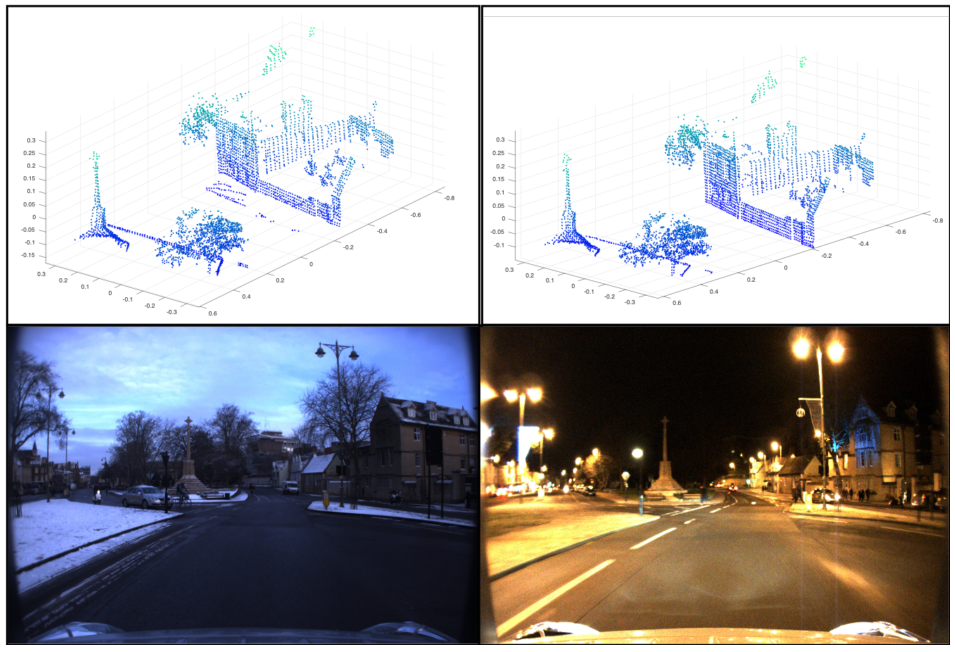
\includegraphics[width=\linewidth]{data_hetero/pointnetvlad.png}
	   		
   		\noindent\rule{\linewidth}{0.4pt}
   		   		
   		\subfigure[][Geometric information]{\label{fig:3d_info}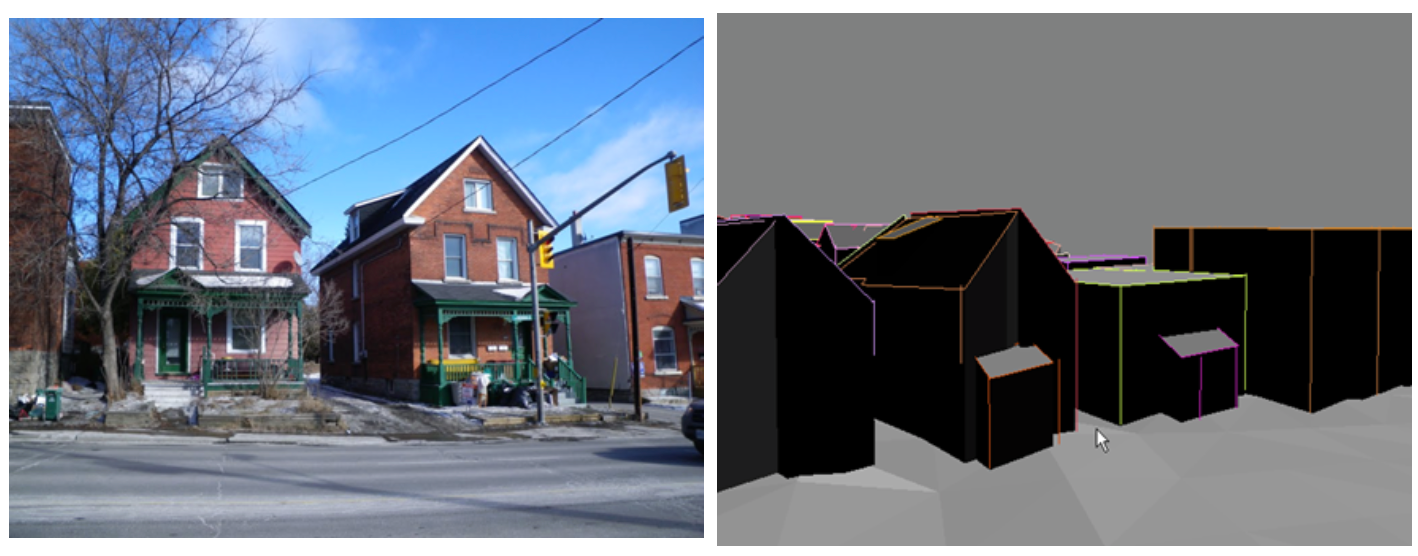
\includegraphics[width=\linewidth]{data_hetero/image_to_DEM.png}}
	\end{minipage}
	\begin{minipage}{0.48\linewidth}
		\centering
   		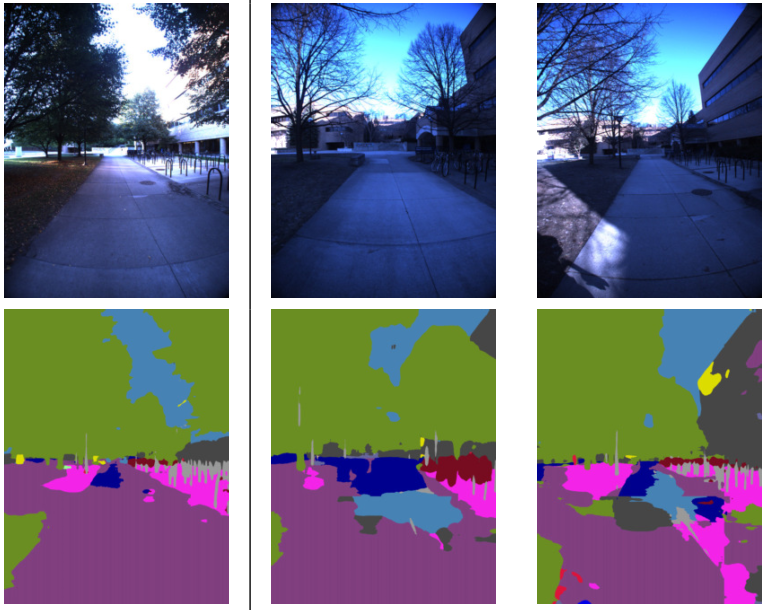
\includegraphics[width=0.95\linewidth]{data_hetero/semantic_vbl.png}
   		
		\noindent\rule{\linewidth}{0.4pt}		
		
   		\subfigure[][Semantic information]{\label{fig:seg_ifo}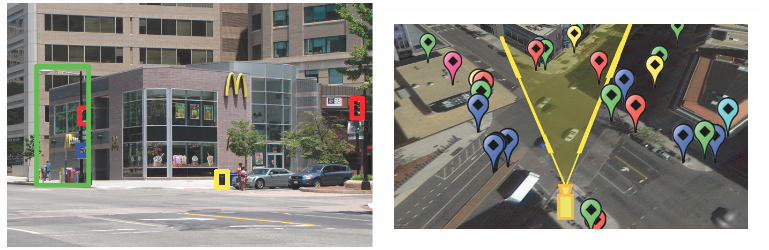
\includegraphics[width=\linewidth]{data_hetero/semantic.png}}
	\end{minipage}
	\caption[Illustration of the data heterogeneity in \ac{vbl}]{\textbf{Illustration of the data heterogeneity in \ac{vbl}:} \ref{fig:3d_info}~From top to bottom: PointNetVLAD~\citep{Uy2018} used to match point cloud for \acs{vbl} and localization system built upon a DEM~\citep{Matei2013}. \ref{fig:seg_ifo}~From top to bottom: data segmentation to help queries (right) to database (left) visual association ~\citep{Schonberger2017a} and localization system with semantic information gathered from OpenStreetMap annotation {Ardeshir2014}. \label{fig:data_div}}
\end{figure}

	Originally, images were the dedicated data modality to \ac{vbl} systems~\citep{Robertson2004}. Still, conventional images for the task of localization have limitations, as mentioned in the previous section (see Section~\ref{sec:changing_environment}). The use of other type of data, such as geometric and semantic information, can circumvent these limitations.

	\subsection{Geometric information}
		\label{subsec:geometric_info}		
		We divide geometric information on three main categories:
		\begin{itemize}
			\item Weak Geometry
			\item Point cloud		
			\item Full Geometry
		\end{itemize}
        
		\paragraph{Weak Geometry}
			\label{subsubsec:weak_geometry}			
			In \citep{Torii2015,Chen2011}, authors introduce weak geometric clues that describe principal 3D planes present in the scene. This information is then used to modify existing images in the database: for rectification purpose~\citep{Chen2011} or to generate more images in order to cover a larger area~\citep{Torii2015}. \citet{Cham2010} use a 2D buildings outline map for \ac{vbl}. From a given image, authors extract buildings corner and match them according to the map. Along the same line, \ac{vbl} method from~\citep{Arth2015} relies on a 2.5D map of Gratz (schematic buildings outlines boxes from OpenStreetMap\footnote{https://www.openstreetmap.org}). 2D map is also used as geo-reference in the work from~\citep{Brubaker2013} (extended version in~\citep{Brubaker2016}) where authors produce, thanks to a stereo-camera, a path of a vehicle that is afterwards matched against the map. The matching process is embedded in a probabilistic framework to handle large environment. \citet{Baatz2012} introduce the use of a \ac{dem} to perform localization in mountainous terrain~\citep{Ramalingam2010,Tzeng2013,Chen2015}. \citet{Bansal2014} extend this idea in urban localization to perform purely geometric \ac{vbl} with images as query input and \ac{dem} of a city as database. These purely geometric descriptions, also used in~\citep{Matei2013,Christie2016,Ramalingam2010,Ramalingam2011} (see figure~\ref{fig:3d_info}), permit localization independently of the illumination conditions (compared to optically dependant methods, see \S\ref{para:illum}).

		\paragraph{3D geometry}
        \label{subsubsec:3d_geometry}
			Previous section \S\ref{subsec:sfm_methods} emphasizes the growing importance of colourized point clouds obtained by \ac{sfm} in \ac{vbl}. Because such geometric models are built upon images collections, reconstructed point clouds also lie on two categories: homogeneous~\citep{Kendall2015,Kendall2016} and heterogeneous~\citep{Irschara2009,Sattler2011} models (see \S\ref{para:data_consistency}). The addition of geometric relation by \ac{sfm} improves retrieval performances~\citep{Sattler2012a} and permits precise pose estimation of the query, on the contrary of methods based on vanilla images collections.

			However, \ac{sfm} reconstruction is a costly operation. Rather than preprocessing the visual data to recover the geometry of the scene, appropriate sensors permit a direct capture of a 3D scene (\textit{e.g.} stereo camera, depth camera, laser, lidar, etc.). Raw data from depth sensor are often used to add supplementary information channel to the \ac{vbl} system. Works from~\citep{Ni2009,McManus2014,Wan2014} use disparity map from stereo camera. Several authors~\citep{Shotton2013,Guzman-rivera2014,Glocker2015} used active depth camera that project infra-red pattern to estimate depth. Similar technology is used in~\citep{Li2016a} to perform \ac{vbl} in complete obscurity. Consistent 3D models are also used to perform \ac{vbl} task. For indoor localization, works from \citep{Shotton2013,Pascoe2015} use textured model reconstructed from RGB-D sensor~\citep{Shotton2013} or hand-crafted with dedicated software~\citep{Pascoe2015}. City-scale models are used by \citep{Aubry2014,Poglitsch2015,Pascoe2015a,Pascoe2015b,Caselitz2016} to perform outdoor \ac{vbl}. 

	\begin{table}[t]
	\centering
	\caption[Data heterogeneity in \ac{vbl}]{\label{tab:data_types}\textbf{Data heterogeneity in \ac{vbl}.} Summary of the various types of data used in \ac{vbl}. First row indicates the type of data present in the database and the first column the type of the query confronted to this database. References in \textbf{bold} denote works using semantic interpretation of the data (see \S\ref{subsec:semantic_info}). $^{\dagger}$~Image-retrieval based methods that compare a input image to a set of images. Numerous references not displayed to readability reason. $^{\ddagger}$~Several works consider \ac{vbl} with as an input a set of images from the same scene rather than only one image input.}

	\renewcommand{\arraystretch}{1.1}
	\newcolumntype{M}[1]{>{\centering\arraybackslash}m{#1}}
	\footnotesize{
	\begin{tabular}{|m{0.13\textwidth} || M{0.18\textwidth} | M{0.18\textwidth} | M{0.18\textwidth} | M{0.18\textwidth} |}
          \hhline{-||----}
		\hfill \bf Database		& Images collection 				& Weak geometry					& SfM						& 3D model \\
          \bf Query 			& \S\ref{subsec:visual_info}			& \S\ref{subsubsec:weak_geometry}		& \S\ref{subsec:sfm_methods} 	& \S\ref{subsubsec:3d_geometry} \\
          \hhline{=::=:=:=:=:}
          Image				& Similarity search$^{\dagger}$ \textbf{\citep{Arandjelovic2014a,Garg2017,Mousavian2015,torralba2003context,Ni2009,Weyand2016}} 		& \citep{Baatz2012,Cham2010,Chen2011,Torii2015} \textbf{\citep{Atanasov2016,Ardeshir2014,Arth2015,Castaldo2015,Wang2015}} &  \citep{Arth2009,Donoser2014,Heisterklaus2014,Irschara2009,Feng2016a,Li2010,Li2012,Lu2015,Lynen2015,Middelberg2014,Sattler2011,Sattler2012,Sattler2015,Sattler2016a,Svarm2014,Zeisl2015}	& \citep{Aubry2014,Mason2011,Russell2011} \\
            \hhline{-||-|-|-|-|}
            Several images$^{\ddagger}$	& \citep{Weyand2016,Zamir2010}		& \citep{Brubaker2016} & \citep{Kroeger2014}								& \textbf{X} \\
            \hhline{-||-|-|-|-|}
            Image + Depth				& \textbf{X}						& \textbf{\citep{Christie2016}}						& \textbf{X}								& \citep{Cavallari,Gee2012,Glocker2013,Glocker2015,Guzman-rivera2014,Shotton2013,Valentin2015,Sizikova2016} \textbf{\citep{Fernandez-Moral2013,Salas-Moreno2013}}\\
            \hhline{-||-|-|-|-|}
            SfM				& \textbf{X}						& \textbf{X}						& \citep{Middelberg2014} \textbf{\citep{Lu2015}}				& \textbf{X} \\
            \hhline{-||-|-|-|-|}
	\end{tabular}
	}
\end{table}

	\subsection{Semantic information}
		\label{subsec:semantic_info}
		Robustness and precision brought by geometric information has a significant cost in term on data acquisition, processing power and storage needs. Nevertheless, there is a good alternative and discriminant data representation: the semantic information. Semantic representation has received a growing interest in research community~\citep{Liu2016a}, in particular for robot navigation purpose~\citep{Kostavelis2015}. Semantic-based methods are notably efficient to perform robust \ac{vbl} to all kind of appearance changes. Indeed, by capturing a meaningful information about the scene composition, this approach is by definition invariant to local changes in appearance and in geometry. Semantic information used in \ac{vbl} are classified between two classes: segmentation and categorization. Segmentation involves local methods that recognize within a data sub-parts with a semantic meaning (\textit{e.g.} object detection in an image). On the other hand, categorization can be seen as global descriptors that associated semantic labels to a given data (\textit{e.g.} scenes interpretation~\citep{Deng2009}).
		
		\paragraph{Segmentation}
			The world ``semantic'' can be understood in different ways: \citet{Fernandez-Moral2013} semantic approach consists of extracting planar surfaces in a scene, while in~\citep{Salas-Moreno2013} authors segment a point cloud to extract objects with higher semantic meaning, like chair or table. Semantic approaches encode the data with a graph where nodes represent objects (plan in~\citep{Fernandez-Moral2013}, furnitures in~\citep{Salas-Moreno2013}) and edges spatial relations between objects. Graph representation offers a compressed data representation capable to handle local changes and minor measurement errors~\citep{Stumm2015}. Semantic segmentation is used in~\citep{Lu2015} to narrow the search scope and in~\citep{Ardeshir2014,Castaldo2015,Christie2016} to directly recover the pose of the query (illustration on figure~\ref{fig:seg_ifo}). Works described in~\citep{Arandjelovic2014a,Mousavian2015} consider the re-weighting of extracted local features in image according to the semantic class of the pixel obtained by image segmentation. Using this information, authors reduce the influence of local features that are not semantically robust for \ac{vbl}, like vegetation or cars. In a same manner, \citet{Arth2015} present concrete application of semantic segmentation of an image to reinforce hypothesis about building facades segmentation (the image is segmented with a SVM classifier). On the other hand, several methods rely on annotated map~\citep{Atanasov2016,Wang2015} or Geographic Information System (GIS)~\citep{Ardeshir2014,Castaldo2015,Qu2015} to guide the localization.
	    	
		\paragraph{Categorization}
			Scene categorization~\citep{Wu2009} is a different manner to exploit semantic clues for \ac{vbl}. High level semantic features have been popularized with the augmentation of labelled data and the accessibility of high computation power devices (GPU, Cloud Computing). ImageNet challenge introduced in 2009 by~\citep{Deng2009} permits the emergence of fast and robust classification methods, like the one described in~\citep{Krizhevsky2012}. Image classification produces a sub-sample of semantically identical images associated to a class. In \ac{vbl}, classification can be used to decimate the database in order to proceed in a subsequent step to a more precise pose search. This method is successfully applied in~\citep{Sunderhauf2015}, where the used \ac{cnn} has a dual-purpose: narrowing the search scope by semantic labelling and producing a global descriptor by weight aggregation (see \S~\ref{para:global_cnn}). In~\citep{torralba2003context,Ni2009}, classical learning methods like Gaussian Mixture Models (GMM) or epitome are employed for associating images to a finite number of possible locations. Recent work from~\citep{Garg2017} use semantic categorization in order to establish transition probabilities from a given type of environment to another one. Authors embed this framework in the SeqSLAM algorithm, improving the global system accuracy. Finally, works presented in~\citep{Hays2008,Weyand2016} consider the problem of classification of images at a world-wide level.

	\subsection{Other modalities}
	\label{subsec:other_modalities}        	
	\citep{Lu2016}
	
	\citep{Bonardi2017}
	
	\citep{Rastgoo2018}
		
				
	\subsection{Cross-data localization}
	\label{subsec:cross_data}        
		We have presented so far three different kinds of information that can be used for \ac{vbl}: optical, geometric and semantic. These types of data are commonly used together to improve localization. In this part, we consider the scenario where all types of data are not available at query time, for instance if the database uses more complete representation of the environment than the query input. It is a common scenario because some data are more difficult to acquire or required specific sensors (\eg geometric information). In this case, methods have to deal with asymmetric representation of the environment in term of data type. We denote this problem cross-data \ac{vbl} and classify the methods founded in the literature in two categories: methods using a common description regardless of the type of data and methods projecting one type of data within another data representation space.
		
    	\paragraph{Common description}
    		Features to Points (F2P) \ac{vbl} (see \S\ref{subsec:sfm_methods}) oppose 2D images to 3D point cloud. In fact, all the features are exclusively extracted from images. On the other hand, semantic abstraction permit cross-data comparison by considering semantic object extracted from various types of data: images to 2D building outline map~\citep{Cham2010}, images to map~\citep{Ardeshir2014,Qu2015,Castaldo2015,Brubaker2016}, RGB-D data to \ac{dem}~\citep{Christie2016}, etc. Referring to a similar physical entity, not necessary semantic, is also a manner to link information from various types of data. Images to DEM correspondences is performed in \citep{Bansal2014} based on a method relying on purely geometric clues extracted both in the image and the model. Recent work from \citep{Sizikova2016,Li2017} use joint descriptors to merge RGB and depth data into a single feature.
					
		\paragraph{Data projection}
			Another widely used method for combining data of different types consists of projecting one of the engaged data into the representation space of the other. For instance, lot of methods consider the challenging problem of registering photographies upon 3D models~\citep{Baatz2012,Kendall2015,Arth2015,Pascoe2015,Pascoe2015a,Pascoe2015b}. Similarity comparison is performed thanks to synthetic images generated from the 3D models \citep{Russell2011,Mason2011,Aubry2014,Poglitsch2015}. Notice the synthesis of skyline profiles from DEM in the work of \citet{Baatz2012}. Special attention is paid to placement of the artificial cameras that generate fake 2D views \citep{Irschara2009,Gee2012,Torii2015}: \citet{Aubry2014} generate cameras over a regular grid to cover a maximal area. A pruning is then applied to only keep the most discriminant views.

To conclude this section, the different types of data used in \ac{vbl} methods are summarized in table~\ref{tab:data_types}.


\section{Discussion}
\label{sec:comparison}
	This section aims to highlight common usage and promising research avenues in \ac{vbl}. As \ac{vbl} panorama is wide and varied, we first propose a review of recent datasets and evaluation metrics used for comparing different approaches.
	
	\subsection{Datasets}
		Commonly used datasets in \ac{vbl} are presented in table~\ref{tab:dataset}. Because of the important difference between 6-\ac{dof} pose estimation and \ac{cbir} for localization methods, there exists two kinds of datasets used in \ac{vbl}: list of images (with basic position information or landmark/place tags) and spatially consistent datasets (that can be composed of point cloud or fine geo-referenced images). Notice the growing number of publicly available datasets starring complete 3D scans of large cities~\citep{Menze2015,Maddern2016,Wang2016}. As mentioned earlier, long-term localization in changing environment is an hot topic in robotic research. We observe therefore appearance of several datasets featuring multiple acquisitions of the same place over long period of time~\citep{Maddern2016,Carlevaris-Bianco2016,Krajnik2010,Krajnik2014}.
		
		For landmarks recognition in city (used method come mainly from \ac{cbir} for localization approaches), the revisited version of Oxford and Paris datasets~\citep{Radenovic2018} is the most used dataset. Concerning precise 6-\ac{dof} pose estimation under changing condition for long-term localization, researchers prefer the benchmark from \citet{Sattler2018} that compile multiples long-term focused datasets.
		
		\paragraph{Coverage and consistency.}
		\label{para:coverage_consistency}
		All the application relying on \ac{vbl} do not cover the same area. For instance, a system design for car pose estimation should be able to localize a vehicle in a larger area than a pedestrian \ac{vbl} system should do. Thus, there exists dataset with a coverage spreading from small indoor scenes to world-wide area.
	
		Visual content within a dataset can be uniform, reference and queries are from the same sensor and captured at the same time, or inconsistent, queries have been taken under different condition or with different sensor than the references data. In order to reflect real-life conditions, outdoor datasets are often inconsistent, with visual dissimilarity between queries and references induced by acquisition sensors, dynamic changes in the scene (cars \& pedestrians),  the weather etc. Indoor datasets use more uniform data~\citep{Shotton2013}, thus targeting application like camera re-localization for robot navigation or augmented reality.

		\paragraph{Evaluation Metrics.}
		\label{subsec:evaluation_metric}
			Authors use various types of performances criteria in order to compare \ac{cbir} for localization methods. The recall @$k$, or recall @$k$\%, is the most used metric. It represents the percentage of queries that present a good match within the $k$ or $k$\% top ranked images. A query is considered correctly localized if it lies inside a tolerance radius from its ground truth position (usually 10 to 25m, depending on the dataset).  Usually $k$ is set to 10 or 1\%. If we consider only the top 1 retrieved candidate for evaluation, distance from the ground truth is used as the main precision criteria. For places or landmarks recognition tasks~\citep{Radenovic2018}, \ac{map} is used to evaluate performances.
			
			Concerning 6-\ac{dof} pose estimation methods, authors often simply compute the mean or median of absolute position and orientation error relative to the ground truth. Another criterion can be extracted from the inlier count obtained against a robust geometric verification (for image based localization). A query is considered as successfully matched if enough inliers are found after \ac{ransac}. However, such a metric does not ensure that the data is well localized according to the model~\citep{Sattler2015}. Percentage of well localized images, \ie under a given error threshold (5cm \& 5$^{\circ}$ for indoor scene), is also a current evaluation metric.  Recently, \citet{Sattler2018} introduce a more detailed metric by considering multiple level of precision (from fine to coarse localization) with different thresholds.
			
	 \begin{landscape}
\begin{table}[!ht]
	\centering
	\caption[Currently used datasets in \ac{vbl}]{\label{tab:dataset} \textbf{Currently used datasets in \ac{vbl}.} Depending on the method to be evaluated (\textit{e.g.} direct or indirect), different datasets are used. Data information (pose, type and homogeneity) concern the documents composing the database and not the one used at query time. Data homogeneity refer to the definition given in paragraph~\ref{para:data_consistency}. RGB-D refer to data recorded with depth-cameras and RGB-S to information collected with standard cameras coupled with laser-scan depth estimation. $^{\dagger}$~6 DoF available in~\citep{Sattler2017}.}
	\renewcommand{\arraystretch}{1.1}
	\footnotesize{
		\begin{tabular}{l  l  c  c  c}
      		\hline
			\bf Name		& \bf Application domain	& \bf Data Pose Info.		& 	\bf Data Type	& \bf Data Homog.	  \\
      		\hline
      		\hline
			\href{http://lear.inrialpes.fr/people/jegou/data.php\#holidays}{INRIA Holidays} [dataset]\citep{Jegou2008} & Scene retrieval & No & RGB & No \\
			\href{http://www.robots.ox.ac.uk/~vgg/data/oxbuildings/}{Oxford Buildings} [dataset]\citep{Philbin2007} & Landmark retrieval & No & RGB & No \\
			\href{http://www.robots.ox.ac.uk/~vgg/data/parisbuildings/}{Paris} [dataset]\citep{Philbin2008} & Landmark retrieval  & No & RGB & No \\
			\href{http://image.ntua.gr/iva/datasets/wc/}{World Cities Dataset} [dataset]\citep{Tolias2011} & Image retrieval & GPS & RGB & No \\
            \href{http://www.ok.ctrl.titech.ac.jp/~torii/project/repttile/}{Pittsburgh 250k} [dataset]\citep{Torii2013} & Image retrieval & GPS & RGB & Yes \\
            \href{https://purl.stanford.edu/vn158kj2087}{San Francisco Landmark} [dataset]\citep{Chen2011} & Landmark retrieval & GPS$^{\dagger}$ & RGB & Yes \\[3pt]

			\href{http://crcv.ucf.edu/projects/GMCP_Geolocalization/}{Pittsburgh Street View} [dataset]\citep{Zamir2014} & Image retrieval & GPS + Compass & RGB & Yes \\
			\href{http://www.ok.ctrl.titech.ac.jp/~torii/project/247/}{Tokyo 24-7 dataset} [dataset]\citep{Torii2015} & Image retrieval & GPS + Compass & RGB & No \\[3pt]

			\href{https://nrkbeta.no/2013/01/15/nordlandsbanen-minute-by-minute-season-by-season/}{Nordland train dataset} & Inter-season matching & GPS & RGB & No \\
			\href{http://labe.felk.cvut.cz/~tkrajnik/dataset/}{Stromovka dataset} [dataset]\citep{Krajnik2010} & Inter-season matching & Inter-season pair & RGB & No \\[3pt]		

			\href{https://cvg.ethz.ch/research/mountain-localization/}{CH1 dataset} [dataset]\citep{Saurer2016} & Localization in mountain & GPS & RGB & No \\
			\href{https://cvg.ethz.ch/research/mountain-localization/}{CH2 dataset} [dataset]\citep{Saurer2016} & Localization in mountain & GPS & RGB & Yes \\
			\href{http://cphoto.fit.vutbr.cz/geoPose3K/}{GeoPose3K} [dataset]\citep{Brejcha2017a} & Localization in mountain & 6 DoF Pose & RGB & No \\[3pt]
			\href{http://mi.eng.cam.ac.uk/projects/relocalisation/\#dataset}{Cambridge Dataset} [dataset]\citep{Kendall2015} & Camera localization & 6 DoF Pose & SfM & Yes \\
			% Rajouter Vienna dataset (homogen si je m'en souviens bien, je trouve pas le lien vers le DS
			\href{http://www.cs.cornell.edu/projects/p2f/}{Rome16K} [dataset]\citep{Li2010} & Camera localization & 6 DoF Pose & SfM & No \\
			\href{http://www.cs.cornell.edu/projects/p2f/}{Dubrovnik6K} [dataset]\citep{Li2010} & Camera localization & 6 DoF Pose & SfM & No \\
			\href{https://www.graphics.rwth-aachen.de/software/image-localization}{Aachen} [dataset]\citep{Sattler2012a} & Camera localization & 6 DoF Pose & SfM & No \\
			\href{http://phototour.cs.washington.edu/datasets/}{Notre Dame dataset} [dataset]\citep{Snavely2006} & Camera localization & 6 DoF Pose & SfM & No \\[3pt]
			\href{https://www.microsoft.com/en-us/research/project/rgb-d-dataset-7-scenes/}{7 scenes} [dataset]\citep{Shotton2013} & Multi-purpose (indoor) & 6 DoF Pose & RGB-D & Yes \\
			\href{https://strands.pdc.kth.se/public/Witham_Wharf_RGB-D_dataset/}{Witham Wharf dataset} [dataset]\citep{Krajnik2014} & Multi-purpose (indoor) & 6 DoF Pose & RGB-D & No \\		
			\href{http://robots.engin.umich.edu/nclt/}{North Campus dataset} [dataset]\citep{Carlevaris-Bianco2016} & Multi-purpose & 6 DoF Pose & RGB-S & No \\			\href{http://mrg.robots.ox.ac.uk/the-oxford-robotcar-dataset/}{Oxford Robotcar} [dataset]\citep{Maddern2016} & Multi-purpose & 6 DoF Pose & RGB-S & No \\
			\href{?}{TorontoCity dataset} [dataset]\citep{Wang2016} & Multi-purpose & 6 DoF Pose & RGB-S & Yes \\
			\href{http://www.cvlibs.net/datasets/kitti/}{KITTI dataset} [dataset]\citep{Menze2015} & Multi-purpose & 6 DoF Pose & RGB-S & Yes \\
			\hline	
		\end{tabular}
	}
    \footnotetext[4]{6 DoF available in~\citep{Sattler2017}}    
\end{table}
\end{landscape}

	\subsection{Runtime consideration}
		\label{subsec:runtime}
		Real-time performances and embedded architectures are constraints mainly present in the robotic community. In \ac{vbl}, such criteria are not always taken into account. This can be explained by the fact that recovering the localization of an input query is a one-shoot action; i.e. it has to be performed only once compared to tracking systems~\citep{Marchand2016} or SLAM algorithms~\citep{Garcia-Fidalgo2015}. Furthermore, more and more embedded systems rely on deported architecture or cloud computer, resolving the problem of low computational power of portable devices~\citep{Middelberg2014}. Yet, some authors manage to reduce the computational cost of their system~\citep{Shotton2013,Glocker2015,Lynen2015}: for instance \citet{Feng2016a} introduce a light version of F2P method and works from~\citep{Weyand2016,Kendall2015,Contreras2017} embed their localization system in a compact CNN architecture loadable on a smart-phone.
			
	\subsection{Trends in VBL}
		\label{subsec:qualitative_comparison}
    	
		A quantitative comparison between all \ac{vbl} systems is impossible due to the diversity in both methods and applications. Nevertheless, we refer reader to recent papers that quantitatively compare specific types of state-of-the-art methods. Concerning indirect methods, following recent contributions~\citep{Radenovic2016,Gordo2016} show comprehensive comparisons. Direct F2P methods based on \ac{sfm} are carefully compared on three papers~\citep{Feng2016a,Sattler2016a,Svarm2016} and \citet{Kendall2017} propose a detailed comparison between \ac{sfm}-direct methods (\S\ref{subsec:sfm_methods}) and \ac{cnn}-direct methods (\S\ref{para:cnn_regressor}). In \citep{Brejcha2017}, authors propose an overview of both indirect and direct \ac{vbl} methods by reporting results of various works in a common table. Finally, \citet{Sattler2017} present the first comparison between indirect and direct methods based on images collection for the task of query accurate localization. In the following, we propose our qualitative analysis of \ac{vbl} panorama. 
        
        \paragraph{From indirect to direct methods}
        	As discussed earlier, there is a trade-off between the area covered and the precision reached by the \ac{vbl} system; the survey of \citet{Brejcha2017} provides a complete overview of this problem. Indirect methods prioritize the space coverage, city scale~\citep{Gordo2016} to word-wide~\citep{Weyand2016}, whereas direct methods focus on precision and exact 6 \ac{dof} estimation~\citep{Feng2016a}. This survey describes \ac{vbl} methods in a chronological order, that is why we present indirect methods before direct ones. However, during the last decade, research focus seems to have turned to direct methods. This can be explained by the drastic increase of applications using precise~\ac{vbl} for both professional (\textit{e.g.} robotics~\citep{Majdik2013}) and individual (\textit{e.g.} augmented reality~\citep{Arth2015}) purposes.
        
        \paragraph{The growing importance of geometric data}
        	Limitations of methods using only images have been discussed in Section~\ref{sec:changing_environment}, and the growing accessibility of geometric data promotes the development of systems based on depth information~\citep{Paparoditis2012}. Furthermore, geometric data facilitates the final pose estimation, which also explains the rapid development of direct methods~\citep{Kroeger2014,Pani2015Lmi,Pani2015Robust}. When available, depth information can directly improve the result of \ac{vbl} methods~\citep{Ni2009,Gee2012,Shotton2013,Torii2015,Cavallari}. Point clouds remain the favourite type of geometric data in~\ac{vbl}~\citep{Sattler2016a}, nevertheless less complete but more compact models have shown promising result for some applications~\citep{Ramalingam2010,Bansal2014,Christie2016,Torii2015}.

        \paragraph{Emergence of semantic localization}
        	Less used in \ac{vbl}, semantic data offer promising results~\citep{Ardeshir2014,Castaldo2015,Christie2016}. In addition to being generic regarding the original ``raw'' scene representation, semantic abstraction permits a discriminative and robust description of the scene. Moreover, the use of semantic graph representations can handle huge amount of data. Loss in area coverage granted by the use of direct methods and complex data can be balanced by semantic information. Indeed, in \citep{Ardeshir2014,Lu2015} authors initially narrow the research scope with extracted semantic clues.
        
        \paragraph{Data combination and cascade schemes}
        	Getting both wide area coverage and high precision of the query pose is the current challenge of \ac{vbl}. Cascade scheme, that can be seen as a combination of indirect and direct methods, are certainly a good alternative to achieve this objective~\citep{Sattler2017}. Indeed, firstly reducing the amount of data and in a second step recovering the exact pose of the query is a well studied topic~\citep{Rubio2015,Azzi2016,Song2016,Meng2016,Sattler2017}. This architecture facilitates the use of heterogeneous data~\citep{Lu2015} in a common framework. Combination of various types of data benefits to the task of \ac{vbl} by exploiting all the available sources of interest present at a given location~\citep{Li2016}.
            
	\subsection{Benefit of heterogeneous data}
    	All along this survey we emphasize the growing importance of multiple types of data (optical, geometric and semantic information) for the task of \ac{vbl}. As discussed in section~\ref{sec:application}, using more sophisticate data aims to overcome shortcoming (presented in section~\ref{sec:changing_environment}) of only-optical based systems. Geometric and depth information permit a total abstraction to the pixel intensity, naturally providing to the system a robustness to illumination variability that can occur in the scene. Local changes in scene appearance and geometry can also be handle with the use of a semantic representation. Optical data, though, contain extremely specific information and are much more easier to collect compared to semantic and geometric data. That is why these three aforementioned data should be considered as complementary information. Based on these observations, there is a real benefit of using heterogeneous data to achieve better results in \ac{vbl}.
		
	\subsection{VBL and machine learning} 
    	\ac{vbl} benefits from the recent progress in machine learning. Indirect methods are now dominated by \ac{cnn} approaches~\citep{Radenovic2016,Gordo2016} (see \S\ref{para:global_cnn}). Image description obtained with convolutional networks gathers all the characteristics needed for the task of scene retrieval. New network architecture has been proposed to resolve the direct \ac{vbl} problem (presented in \S\ref{para:cnn_regressor}). Despite the simplicity and the robustness of these methods, state-of-the-art direct localization results are still obtained through point to feature approaches~\citep{Walch2016a}. However, active researches are pursuing in this promising direction~\citep{Liu2016,Jia2016,Kendall2017}. The last \ac{vbl} sub-domain improved by \ac{cnn} is the semantic scene segmentation and categorization used in some localization methods~\citep{Salas-Moreno2013,Ardeshir2014,Arth2015,Christie2016}. Conventional methods, like Deformable Parts Model (DPM)~\citep{Ardeshir2014}, SVM~\citep{Arth2015} or Automatic Labelling Environment (ALE)~\citep{Christie2016}, should be quickly replaced by CNN~\citep{Sunderhauf2015a,Zhao2016}.
\end{document}
% !TeX spellcheck = en_US
\documentclass[thesis.tex]{subfiles}
\begin{document}

\acresetall

\graphicspath{{3_side_modality_learning_for_localisation/figures/}}

\chapter[Localization in challenging condition]{Image descriptor for localization in challenging condition}\label{chap:3}

In this chapter, we introduce the first step of our hierarchical localization method: a \ac{cbir} method tuned for localization (see section~\ref{subsec:vbl_as_image_retrieval}). More precisely, we are interested in the design of a efficient global image descriptor for long-term localization.

As discussed in the previous chapter, one of the main challenges of \ac{vbl} remains the mapping of images acquired under changing conditions: cross-season images matching~\cite{Naseer2017a}, comparison of recent images with reference data collected a long time ago~\cite{Toft2018}, day to night place recognition~\cite{Torii2015}, etc. Recent approaches use complementary information in order to address these visually challenging localization scenarios: geometric information through point cloud~\cite{Sattler2018,Schonberger2017a} or depth maps~\cite{Christie2016} and semantic information~\cite{Ardeshir2014,Christie2016,Naseer2017a}. However geometric or semantic information are not always available or can be costly to obtain, especially in robotics or mobile applications when the sensor or the computational load on the system is limited, or in digital humanities when the data belong to ancient collections. 

In this work, we are considering a scenario where we have an offline access to multi-modal data but only-radiometric information during the online localization step (as illustrated in figure~\ref{fig:data_setup}). This is a realistic scenario: a mobile mapping vehicle with multiple sensors is used once to gather initial information on the area of interest and then, agents are sending localization request with a low computational sensor like a smart-phone camera. Such setup is also in accordance with the specifications of the \ac{plat} project (see section~\ref{subsec:platinum}), where this works is part of.

Based on these observations, we propose an image descriptor capable of reproducing the underlying scene geometry from a monocular image, in order to deal with challenging outdoor large-scale image-based localization scenarios. We introduce dense geometric information as side training objective to make our new descriptor robust to visual changes that occur between images taken at different times. Once trained, our system can be used on monocular images only to construct an expressive descriptor for image retrieval. This kind of system design is also known as side information learning~\cite{Hoffman2016}, as it uses geometric and radiometric information only during the training step and pure radiometric data for the image localization.  

The chapter is organized as follows. In section~\ref{sec:cbir_data_for_loc}, we first revisit recent works related to image description for localization and side information learning approaches. In section~\ref{sec:preliminary_work}, we describe steps that have led to the design of strong image descriptor trained with side depth information. In section~\ref{sec:impl_details} we give insight on our implementation and on the dataset we used and we illustrate the effectiveness of the proposed method on six localization scenarios in section~\ref{sec:experiments}. We discuss, in section~\ref{sec:chall_loc}, about the challenging night to day image matching problem and, in section~\ref{sec:modality_ref}, we present a variation of our method using dense object reflectance map instead of depth maps. Section~\ref{sec:conclusion} finally concludes the chapter.

\begin{figure}
	\centering
		
	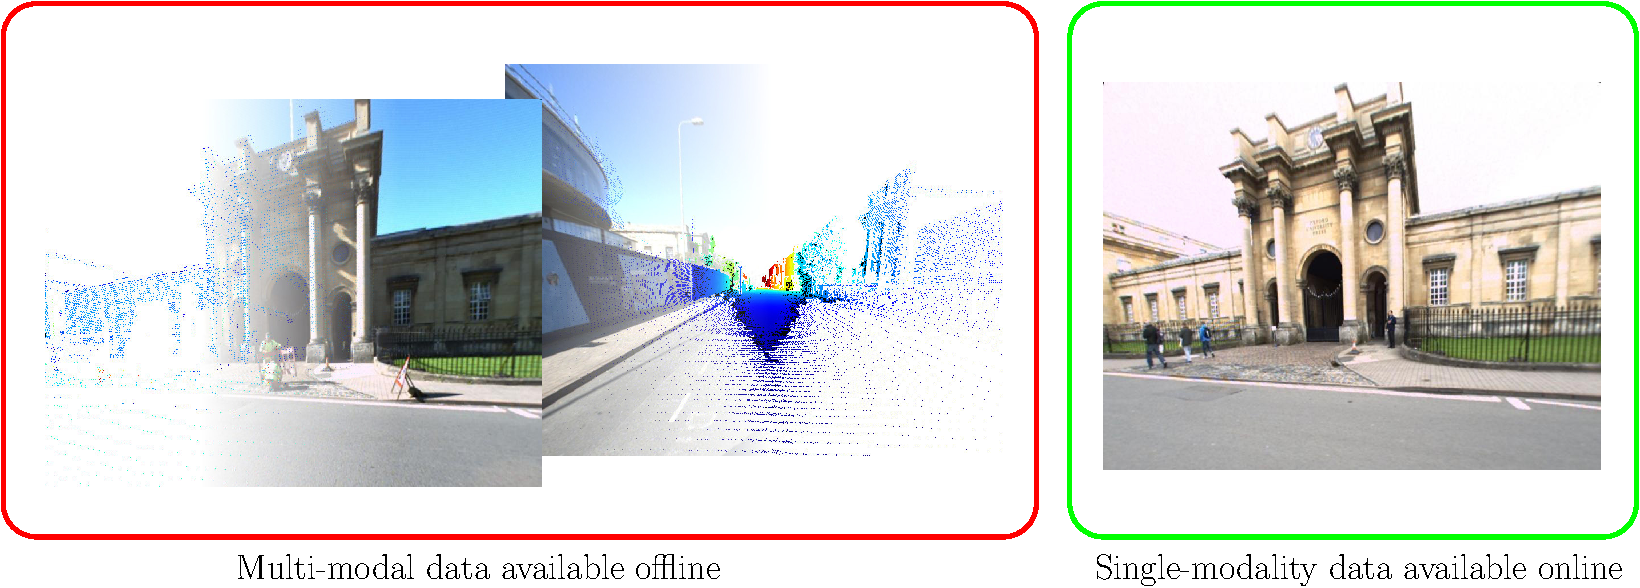
\includegraphics[width=\linewidth]{introduction/data_setup}

	\caption[Data partitioning]{\label{fig:data_setup} \textbf{Data partitioning within a practical localization scenario:} data available offline are richer than the one used during the localization task. We consider RGB (radiometric) + D (geometric) + R (material reflectance) as multi-modal data and only-RGB as single modality information.}
	
\end{figure}
	
\section{Related work}
\label{sec:cbir_data_for_loc}

\subsection{Image descriptor for localization.}

As described in section~\ref{subsec:vbl_as_image_retrieval} (figure~\ref{fig:cbir_for_localization}), the first step of a \ac{cbir} for localization method is the data description. This can be done by using local descriptor, aggregating local features in a global vector or by computing a global signature from the raw image (section~\ref{sec:image_representation}). In the following we review the two type of features mainly used in the literature: 
\begin{itemize}
	\item aggregated local descriptors,
	\item learned descriptors.
\end{itemize}

\subsubsection{Aggregation of local descriptors}
\label{subsec:features_aggregation}
Local features (\S\ref{subsec:local_feature}) are prompt to produce a large number of descriptors for one single data, making the subsequent similarity search intractable. Hence, features aggregation is performed to reduce the dimensionality of the final descriptor vector. In \ac{vbl}, the aggregation process emphasize specific features that are more beneficial for the localization task.

\paragraph{Quantization.} Quantization methods have been widely adopted in image-retrieval domain since pioneer contribution of \citet{Sivic2003}. They consider the problem of object retrieval in an image described through local features in the same manner as text document research. Words equivalent in image domain becomes local features and a dictionary is build upon a large set of features extracted from visual documents' database. These features are clustered to reduce the size of the dictionary; clusters' centroids are then called visual words. For each visual word in the dictionary, and inverted file is maintained to efficiently retrieve all the data that present this specific visual word. The \ac{bof} associates a vector of the dimension of the dictionary containing the visual word frequency of a specific visual document. With this representation, data similarity can be efficiently computed by a simple inner product of their respective visual word frequency vector.

\paragraph{\ac{bof} improvements.} \ac{bof} original scheme~\citep{Sivic2003} proceeds to a hard assignment from the extracted feature to the nearest visual word in the dictionary. However, depending on where the feature lies inside the Voronoi cell created in the clustering step, hard assignment can deteriorate the representation of the visual document. Soft assignment~\citep{Philbin2008} methods have been considered by associating the feature according to a linear combination of the $k$ nearest visual words. Hamming embedding (HE), introduced by \citet{Jegou2008}, subdivides Voronoi cells and associates to each feature a binary signature to refine its position in the visual vocabulary. This method leads to excellent result in term of accuracy and rapidity and is still used in state-of-the-art \ac{vbl}~\cite{Arandjelovic2014}. Inspired by \ac{fv} formulation~\citep{Perronnin2010}, \citet{Jegou2012} introduce \ac{vlad} representation for image-based retrieval. The difference between feature and its closest visual word is assigned to the final descriptor, instead of the visual word itself. The underlying idea behind VLAD representation have inspired various \ac{vbl} methods~\citep{Kim2015,Torii2015,Arandjelovic2017,Yan2016}. For instance, \citet{Kim2015} introduce PBVLAD method to locally fuse SIFT features detected inside a MSER blob. Novel features aggregation method have been recently presented in~\citep{Jegou2014}.
	
\paragraph{Local features weighting.} The weighting step is supposed to emphasize discriminative features regarding the similarity comparison.	Original method by \citep{Sivic2003} used \textit{tf-idf} weighting, relying on the occurrence frequency of the features in the database. \citet{Jegou2009} handle the problem of intra and inter burstiness of visual words (\ie the fact that a feature is more likely to appear in an image if it has already been detected once) by adapting the weight of the visual words before (inter-burstiness) and during (intra-burstiness) the query process. \citet{Torii2013} tackle the problem of visual burstiness introduced by repetitive structures (abundant in urban environment) and introduce meta-features encompassing several similar descriptors (comparable both in their descriptor vector and their spatial location in the image). Such improvement permits a dense extraction of local features in images, bringing superior result in urban environment \ac{vbl}~\citep{Qu2016,Torii2015}. Another work from \citet{Morago2016} also exploits the redundancy present in buildings facades. Recently, \citet{Arandjelovic2014} improve \textit{tf-idf} scheme by considering the descriptors' density in feature space. With their DisLoc weighing, 7\% of the less discriminative visual words can be removed from the database without impacting the performances of the similarity computation. \citet{Mousavian2015} introduce semantic knowledge in the local feature weighting process, reducing the impact of features associated with non-relevant elements for localization (\ie elements that are likely to change or disappear, such as trees and cars).

\subsubsection{Learned descriptors} \label{subsec:cnn_as_global_desc}
With the recent progress of image representation through deep neural network, learned descriptors have become a key component for numerous visual localization methods~\cite{Sunderhauf2015a, Sattler2017a, Schonberger2017a, Sarlin2018, Sarlin2018a, Germain2019, Paulin2017}. Therefore we decide to build on these recent advances and use a \ac{cnn} based image descriptor as base component of our system.  We review in the following recent advances on learned representation for localization.

\paragraph{Off the shelf models.} One of the first method based on learned model for the task of image retrieval have been introduced in~\citep{Babenko2014}. Authors simply use pooling operation on the features block (= neural code) extracted from a \ac{cnn} to compute the image descriptor (see figure~\ref{fig:cnn_aggregation}). Although not trained for the specific task of image retrieval, such model benefits from initial training on images classification task on a huge amount of data (\eg Imagenet dataset~\citep{Deng2009}). In~\citep{Babenko2014,Sunderhauf2015}, authors show that the most discriminative descriptors for the task of image-retrieval, especially applied to place recognition~\citep{Sunderhauf2015}, are extracted from mid-level convolutional layers instead of last fully-connected layers. 

As shown in figure~\ref{fig:cnn_embedding}, convolutional layers produce features block, composed of several activation maps stacked together. In order to capture a more discriminative representation from these features block, several activation map pooling methods can be applied. \ac{mac}~\citep{Razavian2014a} reduce the features block by aggregating the maximum of each activation maps into a vector. Instead of maximum pooling, \ac{spoc}~\citep{Babenko2015} has shown superior results in image retrieval. More specific pooling method, carefully designed for localization, are presented in the next paragraph.

Learned descriptor can be combined with local or patch detectors, in order to obtain sparse representation of the data. In this case, features extracted from the image can be gathered into a single descriptor, like in the \ac{bof} framework. \ac{vlad} embedding is employed in~\citep{Yan2016}. In~\citep{Panphattarasap2016}, patches are sorted according to their relative position in the image and aggregated in a Landmark Distribution Descriptor to improve the subsequent similarity search. \citet{Zhi2016} exploit the intensity response of each patches to discard descriptors with low intensity.

\begin{figure}
	\centering
	
	
\includegraphics[width=\linewidth]{related_work/enc+vlad}
	
	\caption[]{\label{fig:cnn_aggregation} \textbf{} .}	
	
\end{figure}
\paragraph{Specific architecture.} \label{subsubsec:cnn_aggregation}
\ac{rmac}~\citep{Tolias2016} is an improvement of the precedent \ac{mac} method, consisting of the computation of the \ac{mac} vector over regions of various sizes on the activation map. \citet{Gordo2017} achieve state-of-the-art performances by combining \ac{mac} representation with a custom Region Proposal Network (RPN) that autonomously detects regions of interest on the activation map. They also add a differentiable \ac{pca} layer (implemented with on fully connected layer) for dimension reduction. In~\citep{Radenovic2017}, authors use \ac{gem} pooling, a trade of between mean and max pooling with a trainable parameter controlling the degree of spatial ``focus'' of the network. An entirely trainable aggregation layer, called NetVLAD, have been proposed in~\citep{Arandjelovic2017}. Authors design a differentiable architecture that aim to mimic \ac{vlad} aggregation scheme. In~\citep{Iscen2017}, authors create panorama features by aggregating multiple NetVLAD descriptor in a memory vector. \citet{Kim2017a} use the NetVLAD aggregation layer coupled with an Contextual Reweighing Network (CRN) to downgrade irrelevant features according to their local neighborhood, without the use of any manually annotated data. Along the same lines, \citet{Noh2017} propose the DELF architecture for local features extraction. DELF relies on a self-spatial-attention mechanism to select discriminative local region on the features block. 

\begin{figure}
	\centering

	
\includegraphics[width=\linewidth]{related_work/enc+vlad}
	
	\caption[]{\label{fig:triplet_ex} \textbf{} .}	

\end{figure}
\paragraph{Training routine}
In recent works~\citep{Arandjelovic2017,Radenovic2016, Gordo2016}, authors tackle the problem of fine tuning a pre-trained network for the specific task of similar images association for localization. The shared idea is to construct images triplets composed of an anchor, a positive example (displaying the same scene as the anchor image with small view point or illumination variation) and a negative example (unrelated to the anchor image). An images triplet is presented in figure~\ref{fig:triplet_training}. Then, the training signal aims to enforce similarity between computed embedding of the anchor and the positive example and, conversely, to make the anchor and the negative descriptors far for each other in the embedding space. Multiple loss functions can be used to guide the descriptor training. Triplet ranking loss is used in~\citep{Arandjelovic2017,Gordo2017} while in~\citep{Radenovic2016,Noh2017}, authors choose a contrastive loss. A comprehensive evaluation of different objective functions is given by~\citet{Liu2018}. They also propose a Stochastic Attraction and Repulsion Embedding (SARE) loss function, that enforces both inter-place similarity and intra-place difference within the embedding space. 

\citet{Arandjelovic2017} introduce a weakly supervised training approach, using the Google Time machine engine to automatically create large database of triplets. Work from~\citep{Gordo2017,Noh2017} make use of a large Landmark dataset for triplets creation. In~\citep{Radenovic2016,Radenovic2017}, \ac{sfm} is used to link multiple images over a large panel of places. The geometric verification provided by \ac{sfm} permit to control the overlaps between anchors and positives examples. In metric learning, hard examples mining is an crucial step for creating meaningful embedding space. Hard negative mining is performed in~\citep{Arandjelovic2017,Radenovic2017,Gordo2016} by selecting negative examples that are closer to the anchor in the embedding space. \citet{Iscen2018} introduce a manifold distance to compare dataset examples. Using diffusion, they are able to mine more effective examples compare to standard mining methods.

\subsection{Learning with side information}
As mentioned previously, complementary modalities useful for localization, like geometry or semantic, may not be always available at test time. This could be due to limited resources (\eg with embedded system), different sensors, localization of old data, etc. For this reason, we make available the geometric information used in this work only during the offline training step and we rely on side information learning to benefit from this auxiliary modality at test time. Recent work from~\cite{Li2017b} casts the side information learning problem as a domain adaptation problem, where source domain includes multiple modalities and the target domain is composed of a single modality. Another successful method has been introduced in~\cite{Hoffman2016}: authors train a deep neural network to hallucinate features from a depth map only presented during the training process to improve objects detection in images. The closest work to ours, presented in~\citep{Xu2017b}, uses recreated thermal images to improve pedestrian detection on standard images only. Our system, inspired by~\citep{Xu2017b}, learns how to produce depth maps from images to enhance the description of these images.

\paragraph{Depth from monocular image for localization.} Modern neural networks architectures can provide reliable estimation of the depth associated to monocular image in a simple and fast manner~\citep{Eigen2014, Godard2017, Mahjourian2018}. This ability of neural networks has been used in~\citep{Tateno2017} to recover the absolute scale in a \ac{slam} mapping system. \citet{Loo2019} use the depth estimation produced by a CNN to improve a visual odometry algorithm by reducing the incertitude related to the projected 3D points. In this work, we use the depth information obtained by a neural network as stable features across season changes. \citet{Taira2019} rely on dense surface normal (derivative of the depth map) and semantic segmentation created by a convolutional encoder/decoder~\citep{Zamir2018} for localization of indoor low-textured images.
\section{Preliminary work}
\label{sec:preliminary_work}

\subsection{Motivation}
\begin{figure}
	\centering
		
	\hfill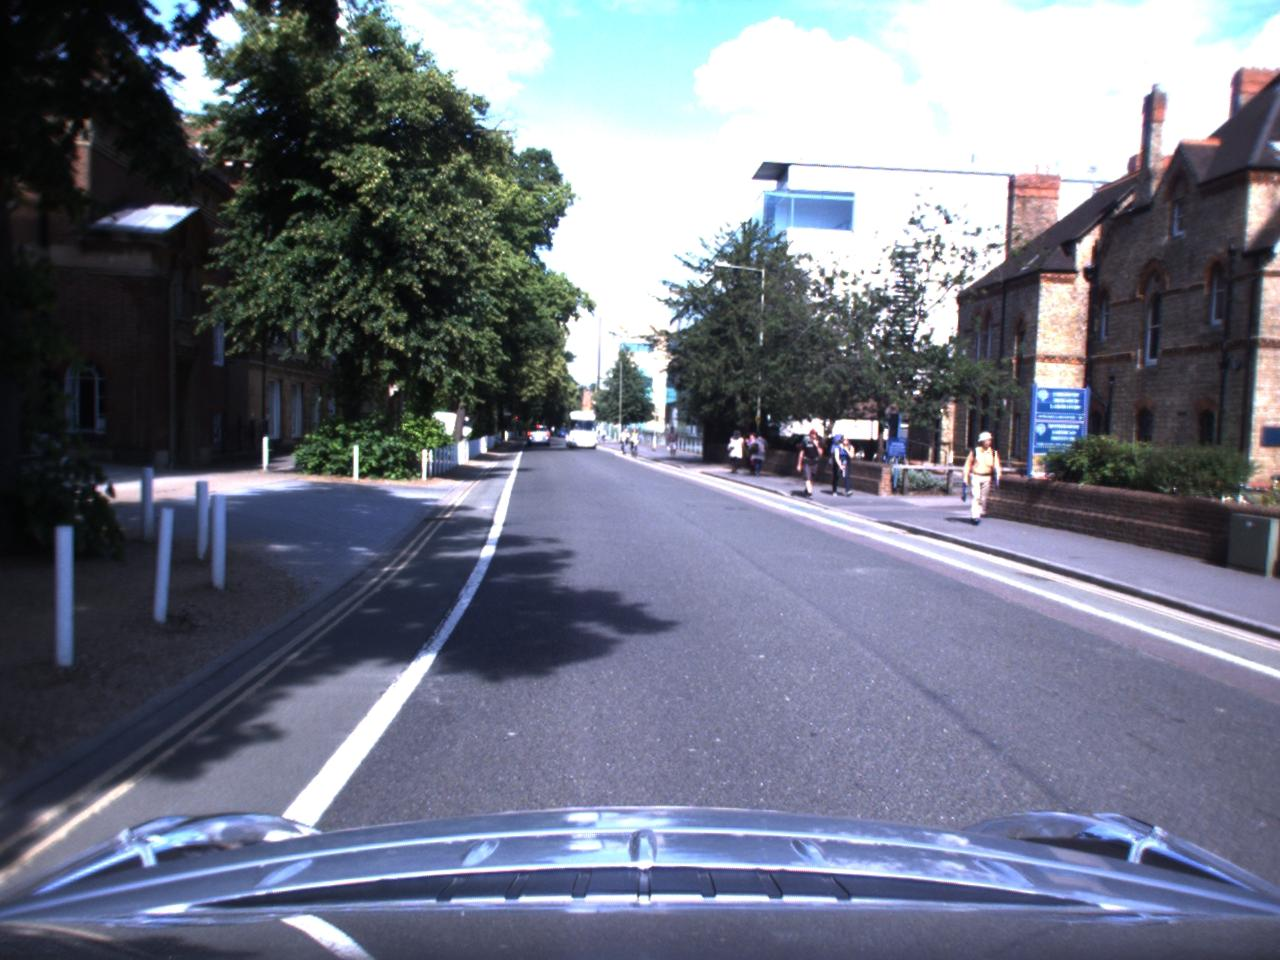
\includegraphics[width=0.25\linewidth]{preliminary/sun}\hfill
	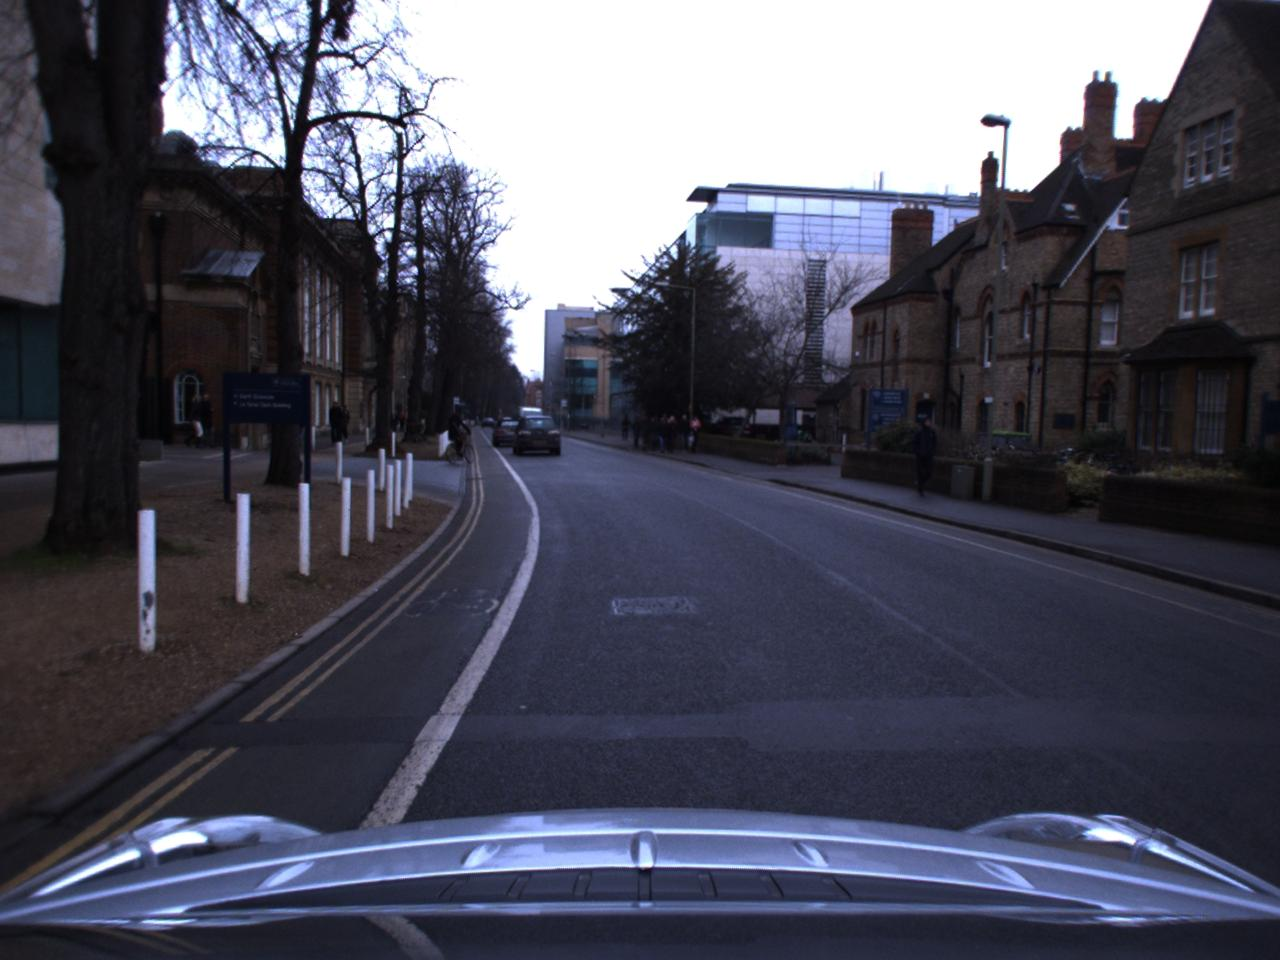
\includegraphics[width=0.25\linewidth]{preliminary/overcast}\hfill
	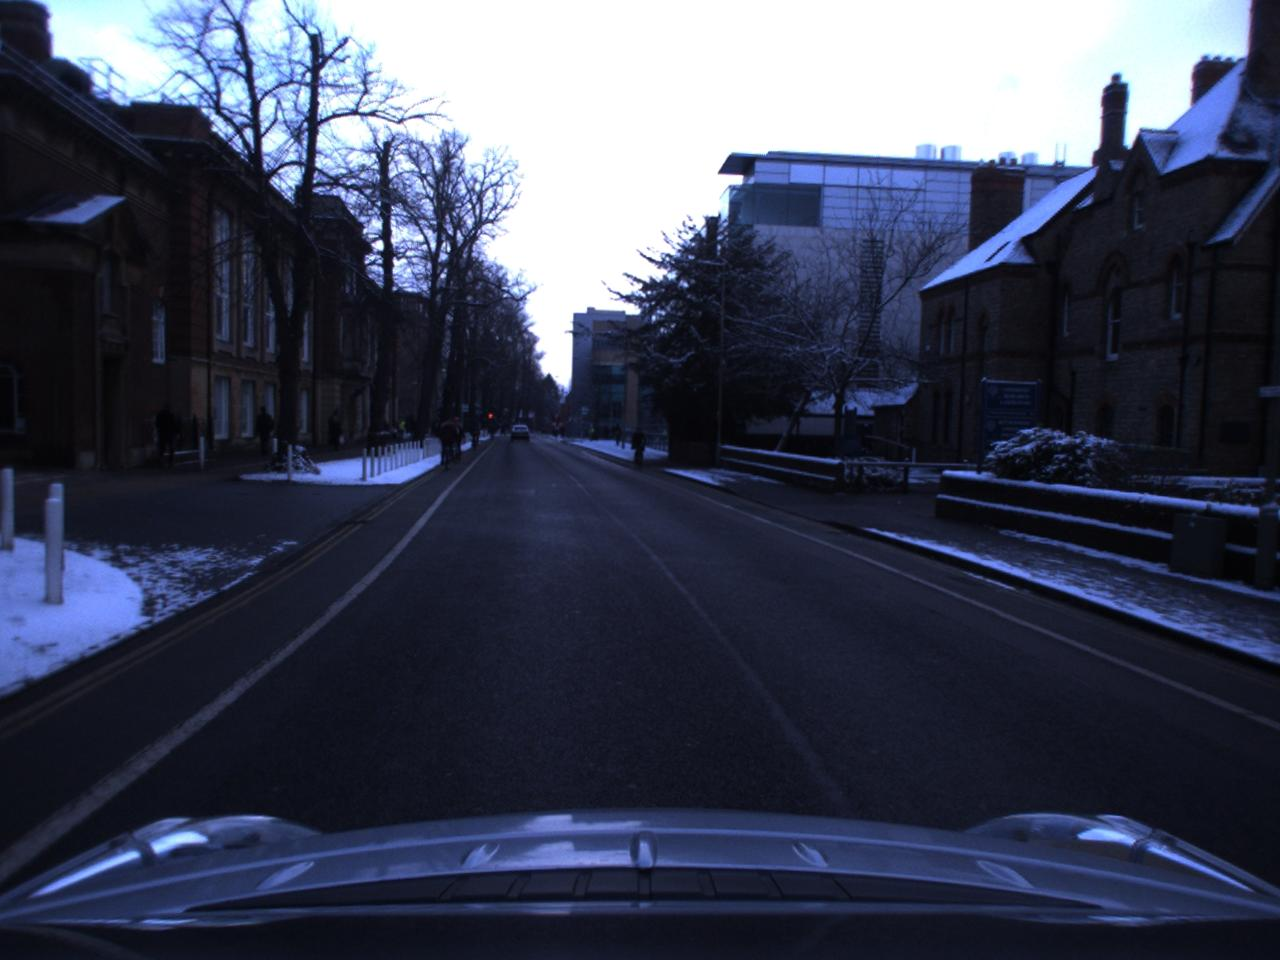
\includegraphics[width=0.25\linewidth]{preliminary/snow}\hfill
	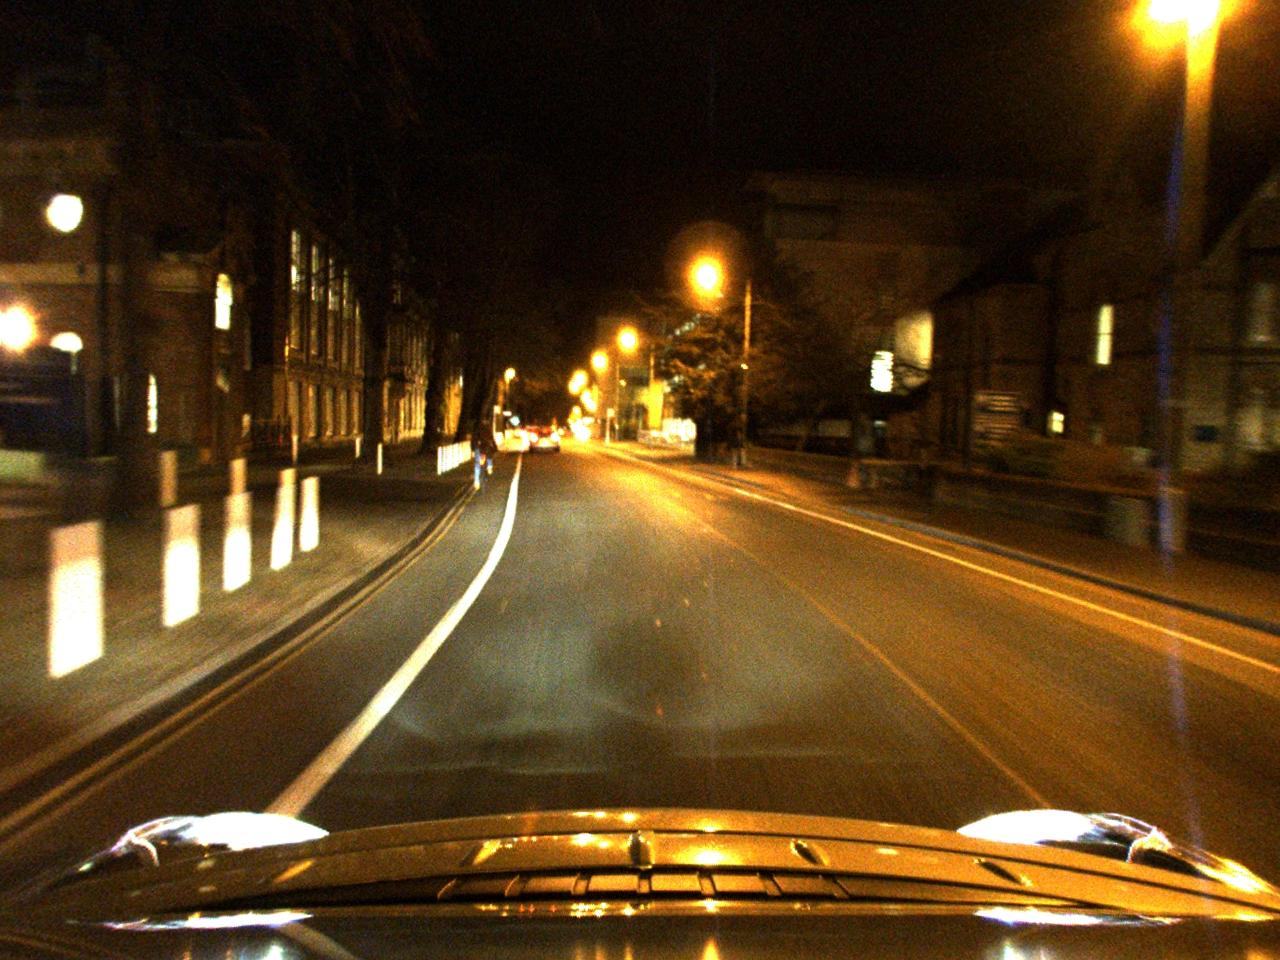
\includegraphics[width=0.25\linewidth]{preliminary/night}\hfill
	
	\hfill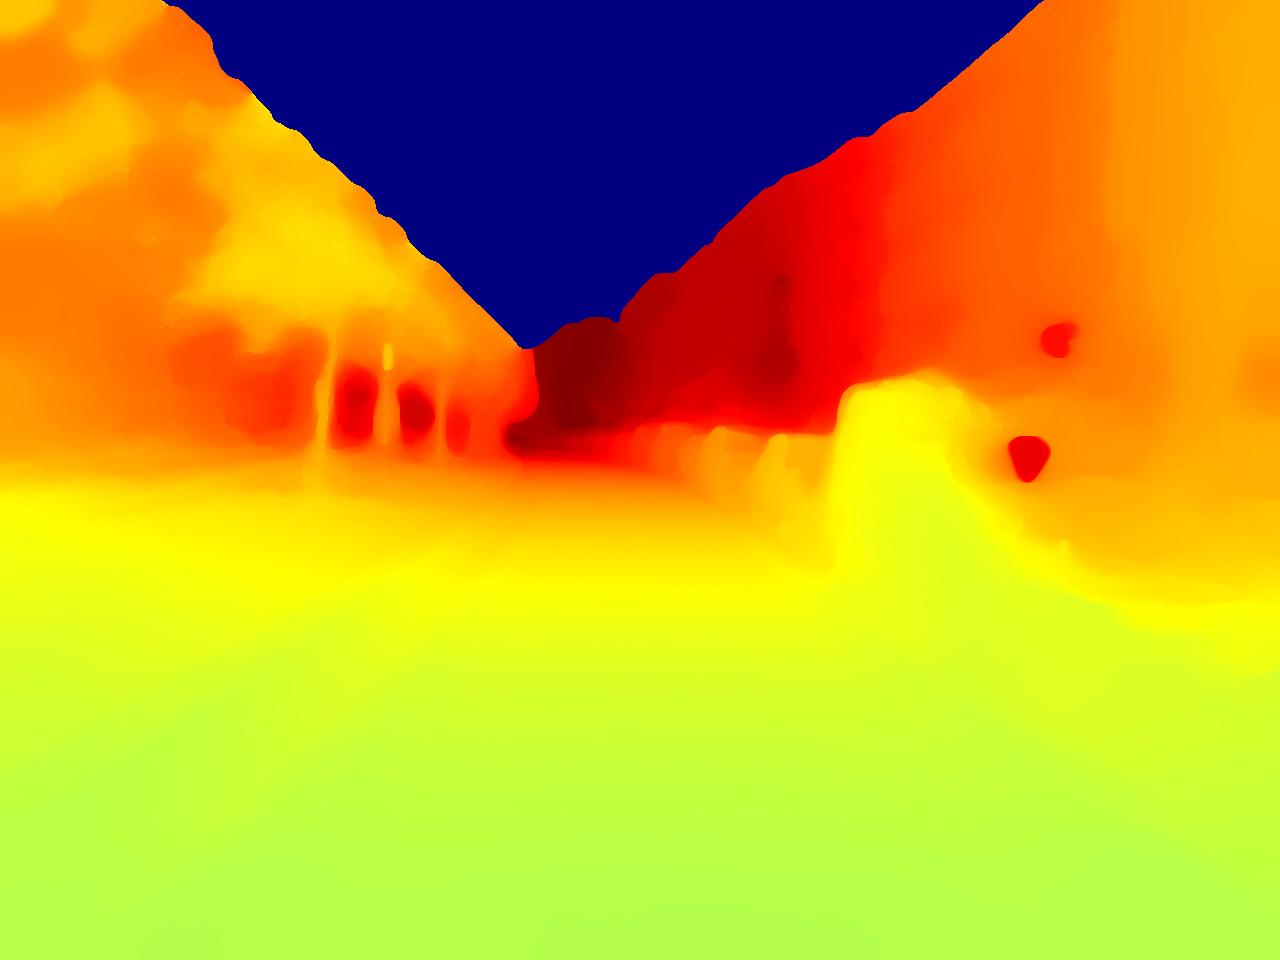
\includegraphics[width=0.25\linewidth]{preliminary/depth}\hfill
	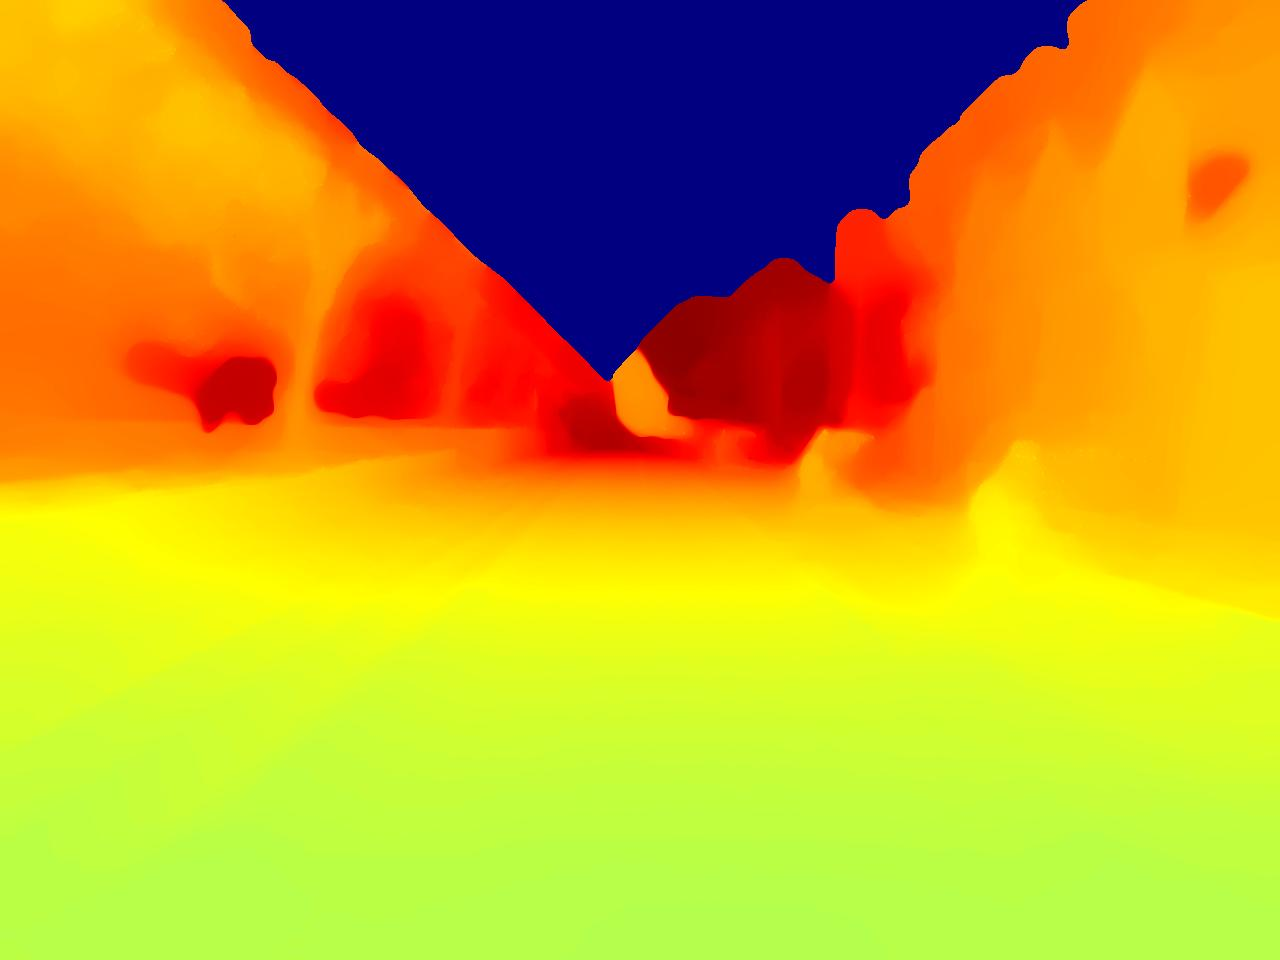
\includegraphics[width=0.25\linewidth]{preliminary/depth3}\hfill
	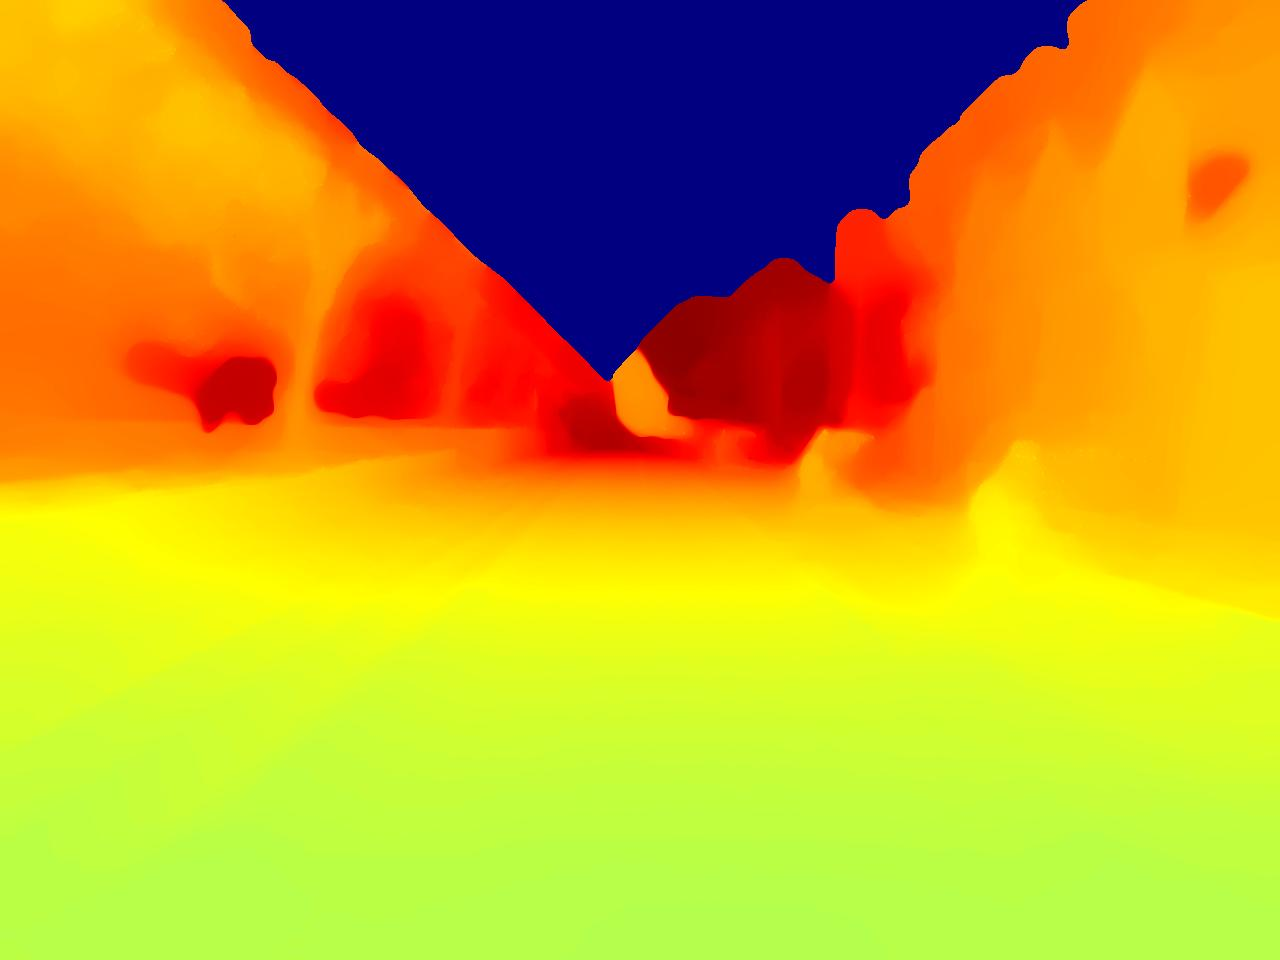
\includegraphics[width=0.25\linewidth]{preliminary/depth3}\hfill
	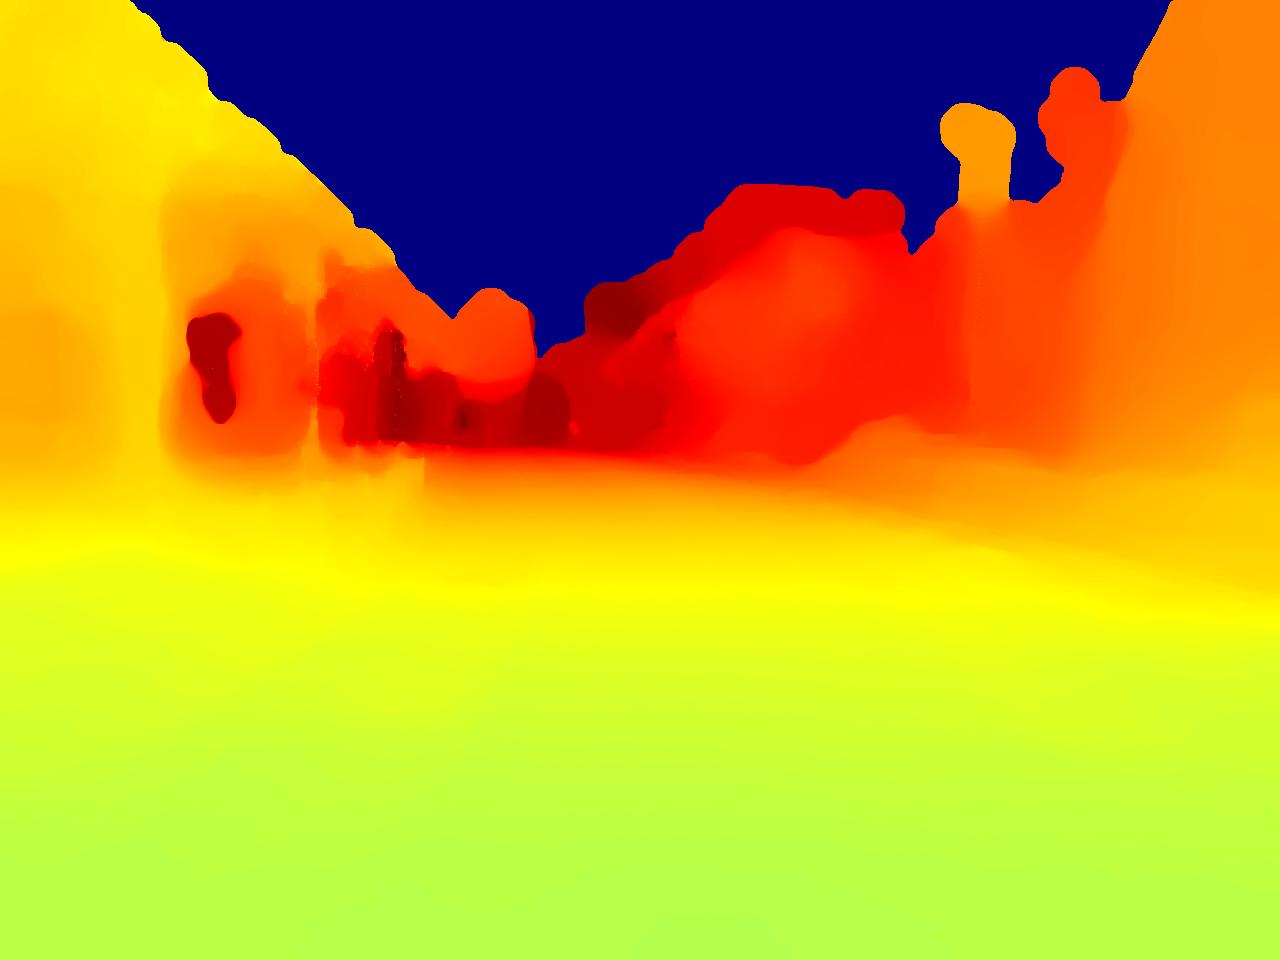
\includegraphics[width=0.25\linewidth]{preliminary/depth4}\hfill

	\caption[Images and depth maps comparison]{\label{fig:image_vs_depth} \textbf{Visual changes between radiometric and geometric domain:} due to outdoor conditions, visual aspect of images changes over time (top row), while, geometry of the scene (corresponding depth maps, bottom row) remains stable.}
	
\end{figure}
	
As illustrated in figure~\ref{fig:image_vs_depth}, outdoor conditions drastically impact visual appearance of a scene. It will be challenging for a descriptor relying only on the radiometric information to associate to the four images of figure~\ref{fig:image_vs_depth} similar embeddings. Thus, if we take a look at the underlying geometry in these images (\ie the associated depth maps, bottom of figure~\ref{fig:image_vs_depth}), this information seems more stable across changing conditions. The central idea of our method is to use recent modality transfer network~\citep{Eigen2014, Godard2017, Mahjourian2018} (from images to depth maps) to provide invariant image representation to our \ac{cnn} descriptor during training. At test time, the trained descriptor can be used on images only.

\subsection{Initial model architecture}
\begin{figure}
	\centering
	
	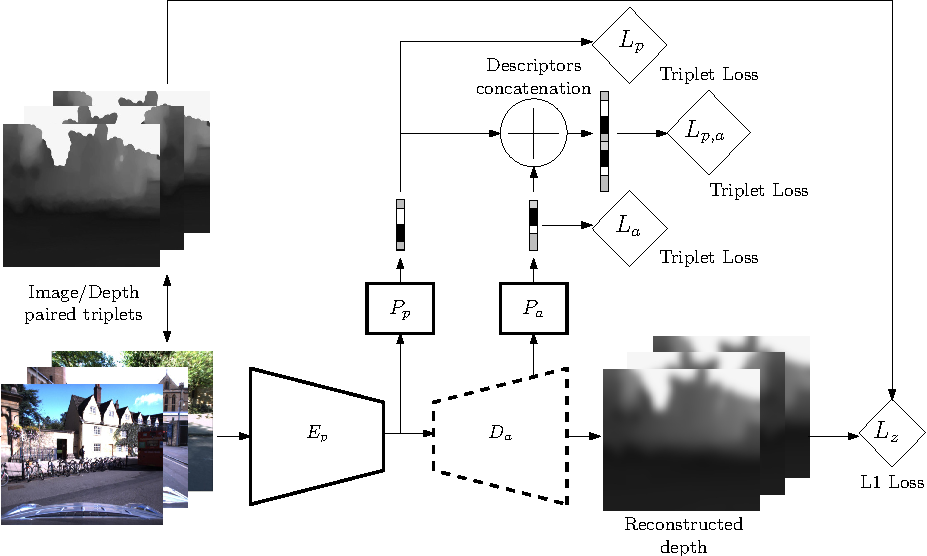
\includegraphics[width=\linewidth]{preliminary/preliminary_method}
	
	\caption[Preliminary solution]{\label{fig:preliminary_method} \textbf{Training pipeline of our preliminary solution.}}
	
\end{figure}
An overview of our method can be seen in figure~\ref{fig:preliminary_method}.

\paragraph{Principal descriptor.}
We build on recent advance in \ac{cnn} image descriptor for designing our system. We use standard convolution features extractor linked to a pooling descriptor layer (figure~\ref{fig:cnn_aggregation}). Formally, we denote $f_p$ the principal features vector of image $x$ computed by encoder $E_p$ and descriptor $P_p$:
\begin{equation}
	\label{eq:desc_details}
	f_p(x) = P_p(E_p(x)).
\end{equation}

We denote $\theta_{p}$ the weights of the image encoder and descriptor $\{E_p, P_p\}$. Notice that descriptor $P$ do not necessary contains trainable parameters (if we consider \ac{mac} pooling method for instance).

Considering the images triplet $\{x, x^+, x^-\}$, as described in previous section (see figure~\ref{fig:triplet_training}), our \ac{cnn} descriptor can be trained with the following triplet ranking loss~\citep{Arandjelovic2017}:
\begin{equation}
	\label{eq:triplet_loss}
	L_p(x, x^+, x^-) = max\left(\lambda + \norm{f_p(x) - f_p(x^+)}_2 - \norm{f_p(x) - f_p(x^-)}_2, 0 \right),
\end{equation}
where $\lambda$ is an hyper-parameter controlling the margin between positive and negative examples.

\paragraph{Side geometry learning.}
In order to recover the geometric information from the radiometric signal, we use a fully convolutional decoder $D_a$~\citep{Eigen2014}. $\theta_{a}$ are the trainable weights of our decoder. Lets $\{x, z\}$ be a pair of image and corresponding depth map, we can train our decoder to compute the depth map from input image with the following loss function:
\begin{equation}
	\label{eq:l1_loss}
    L_z(x,z) = \norm{z - \hat{z}(x)}_{1},
\end{equation}
where $\hat{z}(x) = D_a(E_p(x))$, is the output of the decoder. $L_z$ is a simple pixel loss penalizing absolute error between the output depth map $\hat{z}(x)$ and the target $z$.

\paragraph{Auxiliary descriptor.}
In order to take advantages of the learned depth representation in our final descriptor, we use intermediate deep features computed by $D_a$ to create another descriptor $f_a$:
\begin{equation}
	\label{eq:desc_aux}
	f_a(x) = P_a(\bar{D}_a(E_p(x))),
\end{equation}
where $P_a$ is an auxiliary descriptor and $\bar{D}_a$ designs an intermediate output extracted from decoder $D_a$. We do not use the reconstructed depth map $\hat{z}(x)$ (\ie raw output of $D_a$) to produce vector $f_a(x)$ because it will be to sensitive to small viewpoint variations. Instead, we use an intermediate output from $\bar{D}_a$, that should be more meaningful compared to  $\hat{z}(x)$ and less sensitive to viewpoint changes. Indeed, because the decoder upsample the features maps, output of $\bar{D}_a$ has a smaller spatial resolution and is deeper in comparison to $\hat{z}(x)$. We apply a triplet ranking loss $L_a$ (see equation~\ref{eq:triplet_loss}) to train weights $\theta_{a}$ of decoder $D_a$ and descriptor $P_a$. 

\paragraph{Overall training.}
Finally, we combine the principal and auxiliary features, $f_p(x)$ and $f_a(x)$ in a common vector:
\begin{equation}
	\label{eq:concat_desc}
	f_{p,a}(x) = \left[ f_p(x), f_a(x)  \right],
\end{equation}
where $[ \cdot ]$ is the concatenation operation. Overall optimization is obtained through the last triplet ranking loss $L_{p,a}$ and the final cost function is defined by:
\begin{multline}
	\label{eq:overall_loss}
	L(x, x^+, x^-,z, z^+, z^-) = L_p(x, x^+, x^-) + L_a(x, x^+, x^-) + L_{p,a}(x, x^+, x^-)\\
	 + \frac{1}{3}\left[ L_z(x, z) + L_z(x^+, z^+) + L_z(x^-, z^-) \right].
\end{multline}

Our initial method requires triplets of RGB-D data to be trained.

\subsection{Hallucination network}
\begin{figure}
	\centering
	
	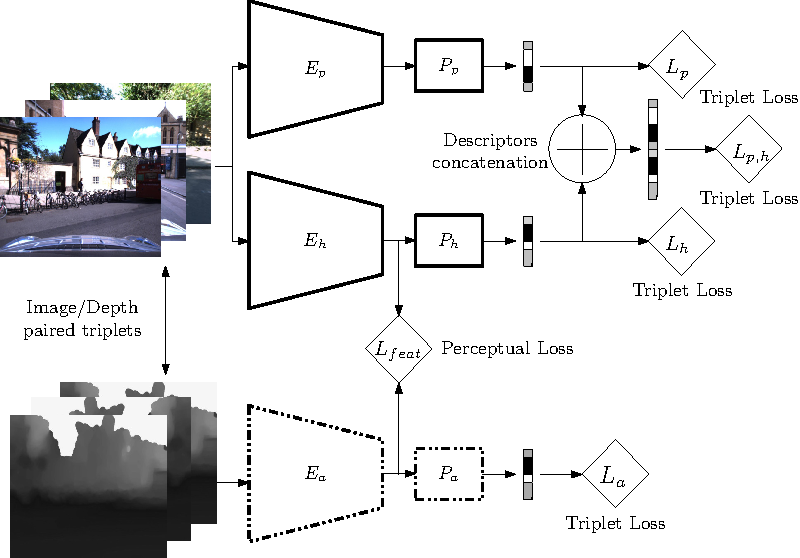
\includegraphics[width=\linewidth]{preliminary/hall_method_training}
	
	\caption[Hallucination network for image descriptors learning]{\label{fig:hall_method} \textbf{Hallucination network for image descriptors learning:} we train an hallucination network, inspired from~\cite{Hoffman2016}, for the task of global image description. Unlike the proposed method (see figure~\ref{fig:our_method}), hallucination network reproduces feature maps that would have been obtained by a network trained with depth map rather than the deep map itself.}
	
\end{figure}

We compare our method of side information learning with a state-of-the-art approach system, named hallucination network~\citep{Hoffman2016}. The hallucination network was originally designed for object detection and classification in images. We adapt the work of~\citet{Hoffman2016} to create an image descriptor system that benefits from depth map side modality during training. Our adaptation of the hallucination network for image description is presented in figure~\ref{fig:hall_method}.

\paragraph{Principal descriptor.}
Similar to our proposal, the system is composed of a principal image descriptor: encoder $E_p$ + descriptor $P_p$, trained jointly through triplet ranking loss of equation~\ref{eq:triplet_loss}.

\paragraph{Auxiliary descriptor.}
Hallucination architecture needs an auxiliary network for training purpose, that will be discarded at test time. This auxiliary branch focus on extracting significant information from the side modality (the depth map in our case). We design the auxiliary network similar to our principal branch: the depth map descriptor is composed of an encoder $E_a$ linked to a descriptor $P_a$. The depth map descriptor is trained with a triplet ranking loss $L_a$, where the embeddings are directly computed from the truth depth maps:
\begin{equation}
	f_a(z) = P_a(E_a(z)).
\end{equation}

\paragraph{Hallucination descriptor.} The key component of \citet{Hoffman2016} proposal is the hallucination network. The task of the hallucination branch is, with images as input, to reproduce feature maps that would have been obtained by a network trained with depth map rather than the depth map itself. The hallucination network share the same architecture as the principal and the auxiliary branches. The hallucination descriptor is composed of an encoder $E_h$ and a descriptor $P_h$ with trainable weights $\theta_h$. It is trained with triplet ranking loss $L_z$ under the constraint of a perceptual loss~\citep{Johnson2016}:
\begin{equation}
	\label{eq:perceptual_loss}
	L_{feat}(x, z) = \norm{E_h(x) - E_a(z)}_2.
\end{equation}
This constraint can be interpreted as knowledge distillation~\citep{hinton2015distilling}. Final image descriptor is obtained by concatenating $f_p(x)$ and $f_h(x)$.

\paragraph{Overall training.} Training routine presented in~\citep{Hoffman2016} is two-step: we first train weights $\theta_a$ of the auxiliary descriptor with loss $L_a(z, z^+, z^-)$ and, secondly, we initialize hallucination weights $\theta_h$ with pre-trained weights $\theta_a$ and minimize the following cost function:
\begin{multline}
	\label{eq:overall_hall_loss}
	L(x, x^+, x^-,z, z^+, z^-) = \alpha\left[ L_p(x, x^+, x^-) + L_h(x, x^+, x^-) + L_{p,h}(x, x^+, x^-) \right]\\
	+ \gamma\left[ L_{feat}(x, z) + L_{feat}(x^+, z^+) + L_{feat}(x^-, z^-) \right],
\end{multline}
where $\alpha$ and $\gamma$ are weighting constants. During final optimization, weights $\theta_a$ are frozen. 

Like our proposal, this method requires triplets of RGB-D data to be trained and, at test time, the principal and hallucination descriptors are used on images only.

\subsection{Preliminary results}


\section{Implementation details}
\label{sec:impl_details}

\begin{figure}
	\centering
	
	\begin{minipage}{0.435\linewidth}
		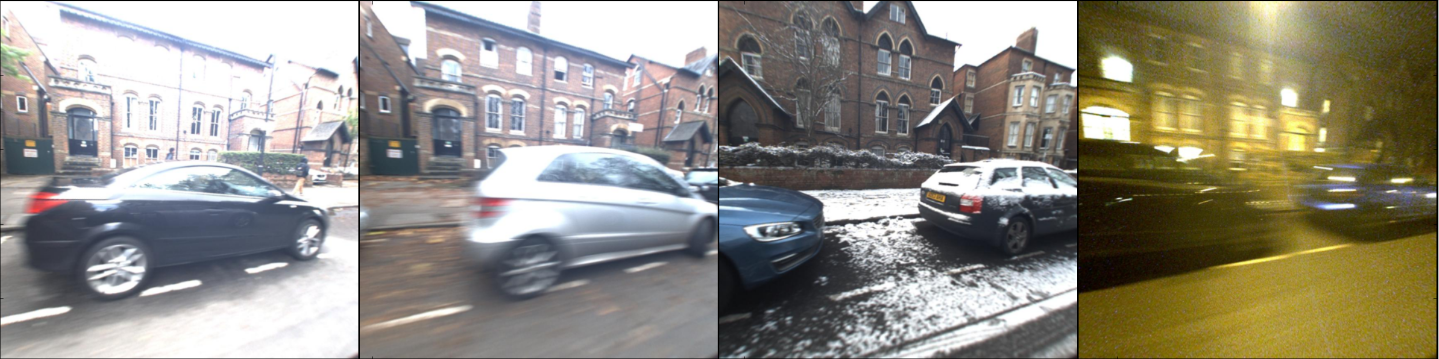
\includegraphics[width=\linewidth]{details/oxf_exs/ex1}
		
		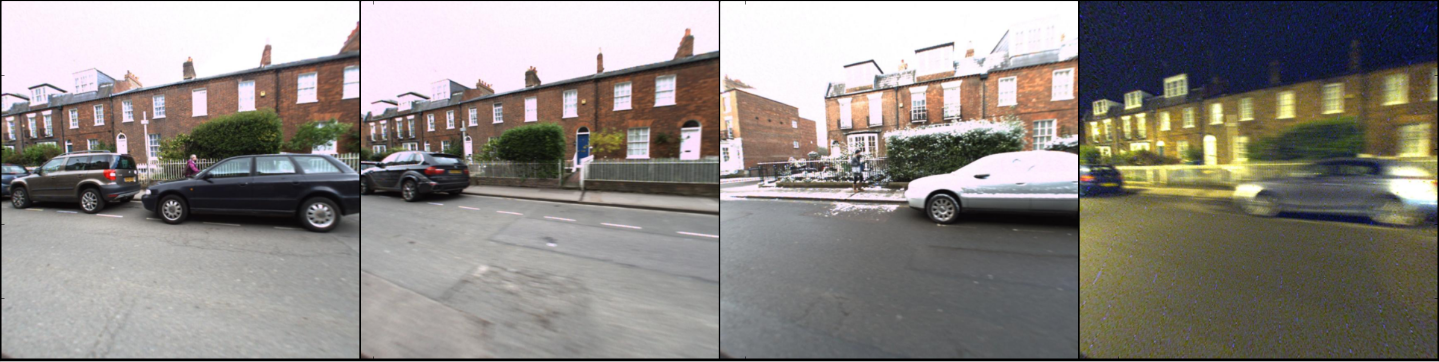
\includegraphics[width=\linewidth]{details/oxf_exs/ex2}
		
		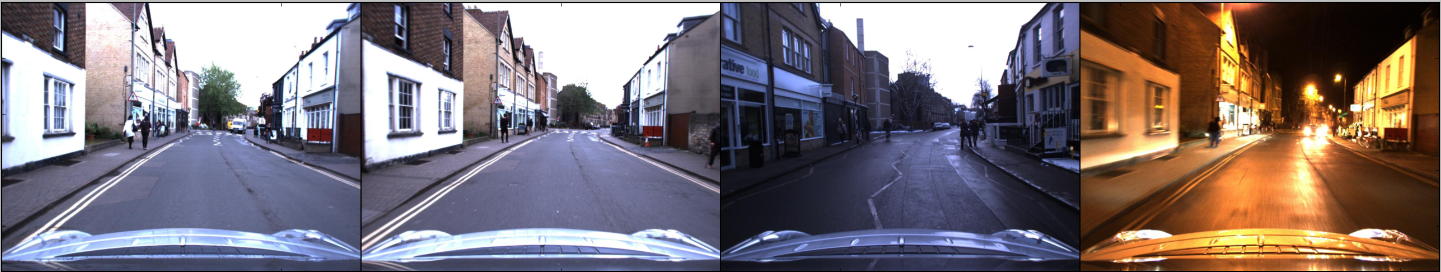
\includegraphics[width=\linewidth]{details/oxf_exs/ex4}
		
		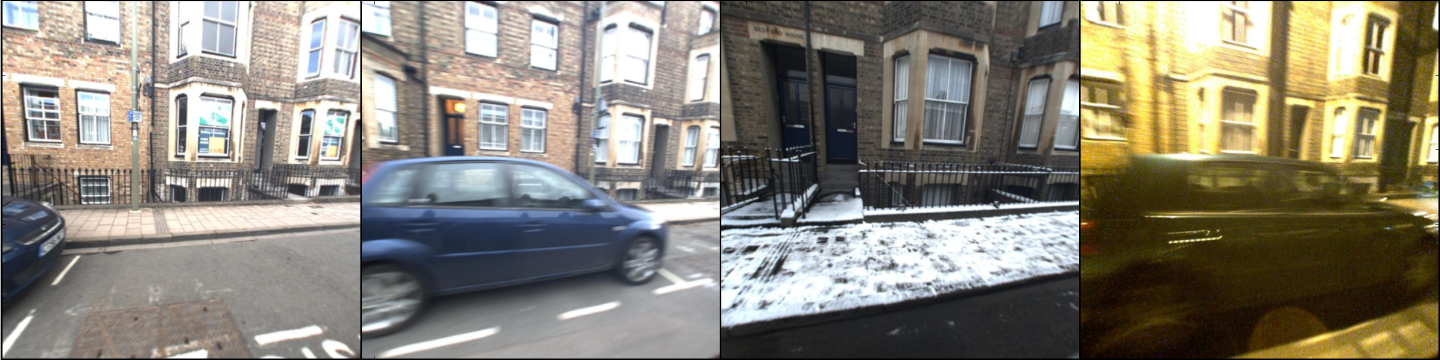
\includegraphics[width=\linewidth]{details/oxf_exs/ex6}
		
		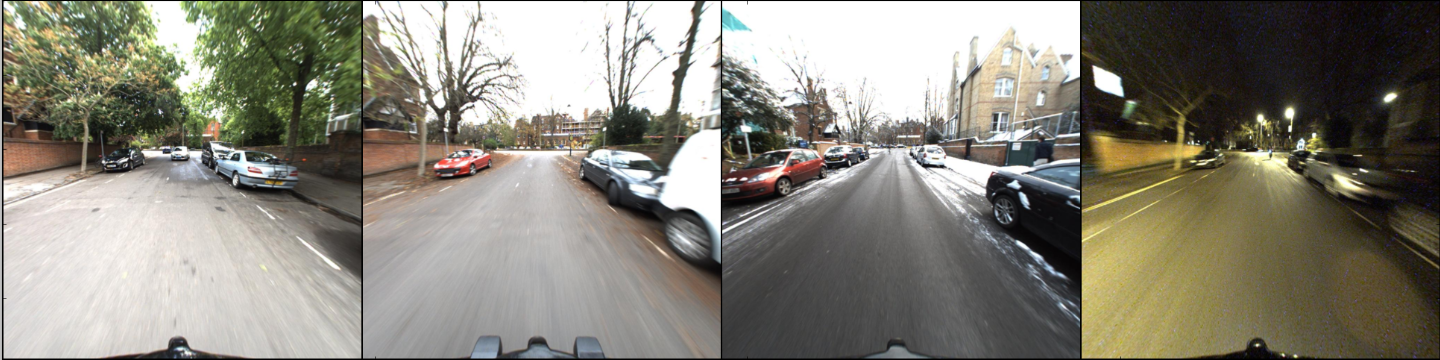
\includegraphics[width=\linewidth]{details/oxf_exs/ex3}
		
		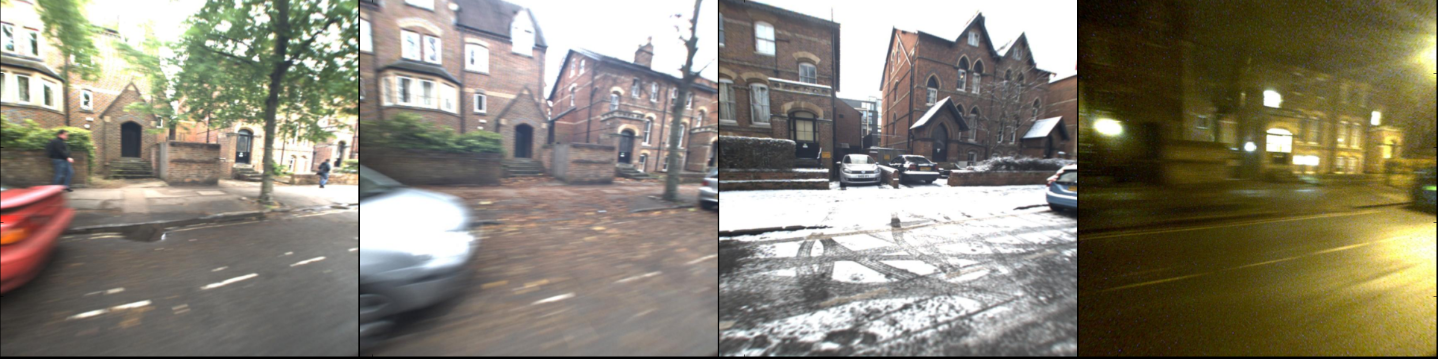
\includegraphics[width=\linewidth]{details/oxf_exs/ex5}
		
		\scriptsize
		\begin{tabularx}
		{\linewidth}{X X X X}
			Reference images & 	Long-term & Snow queries & Night queries
		\end{tabularx}
	\end{minipage}\hfill	
	\begin{minipage}{0.555\linewidth}
		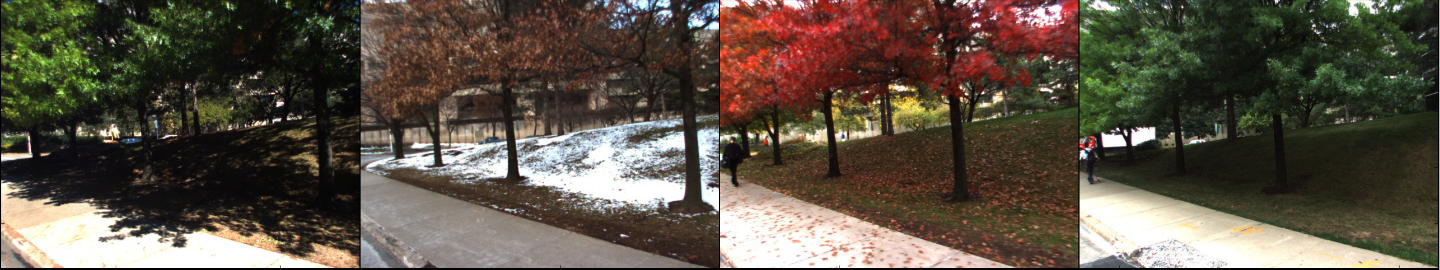
\includegraphics[width=\linewidth]{details/cmu_exs/ex1}
		
		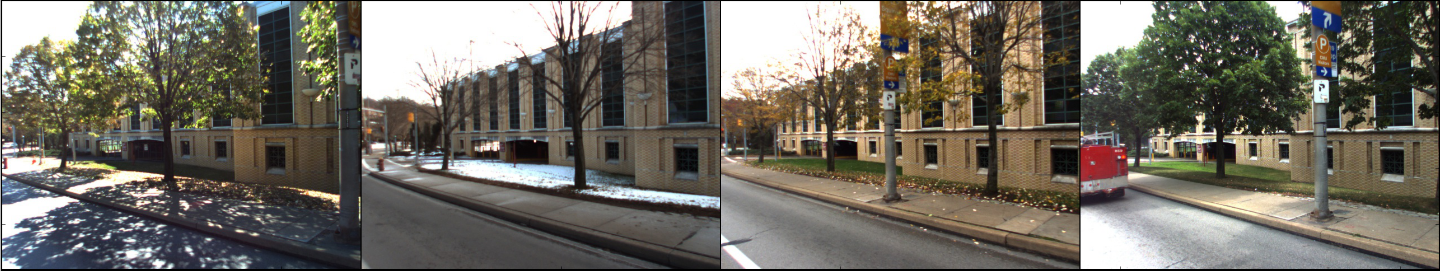
\includegraphics[width=\linewidth]{details/cmu_exs/ex6}
		
		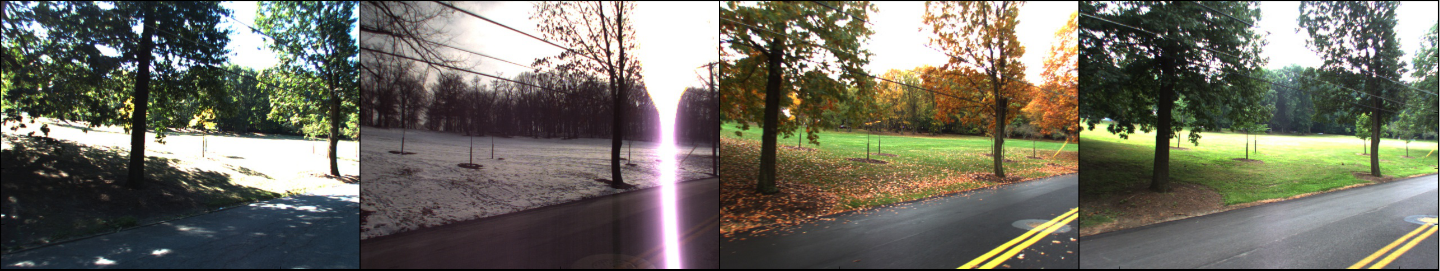
\includegraphics[width=\linewidth]{details/cmu_exs/ex4}	
		
		\includegraphics[width=\linewidth]{details/cmu_exs/ex2}	
		
		\includegraphics[width=\linewidth]{details/cmu_exs/ex3}	
		
		\includegraphics[width=\linewidth]{details/cmu_exs/ex5}	
		
		\scriptsize
		\begin{tabularx}{\linewidth}{X X X X}
			Reference images & Snow queries & Autumn queries & Long-term queries 
		\end{tabularx}
	\end{minipage}

	\caption[Examples of test images]{\label{fig:dataset} \textbf{Examples of test images :} we evaluate our proposal on 6 challenging localization sequences. Query image samples and the closest reference images in the database are presented from Oxford Robotcar~\cite{Maddern2016} (left) and CMU season dataset~\cite{Bansal2014a} (right).}
	
\end{figure}


\subsection{Dataset}
\label{subsec:dataset}
	We have tested our new method on the \textit{Oxford Robotcar} public dataset~\cite{Maddern2016} and the \textit{CMU Visual localization} dataset~\cite{Bansal2014a} from the city of Pittsburg. There are common dataset used for image-based localization~\cite{Sattler2018} and loop closure algorithm involving neural networks training~\cite{Porav2018} under challenging conditions.
		
\subsection{Dense depth maps creation}
Occlusion filter + exps
		
\subsubsection{Training data}
	We use the temporal redundancy present in Oxford Robotcar dataset to build the images triplets to train our CNN. We build 400 triplets using three runs acquired at dates: \texttt{2015-05-19, 2015-08-28} and \texttt{2015-11-10}. We selected an area of the city different from the one used for training our networks for validation.
	Depth modality is extracted from the lidar point cloud. When re-projected in the image frame coordinate, it produces a sparse depth map. Since deep convolutional neural networks require dense data as input, we pre-process these sparse modality maps with inpainting algorithm from~\cite{Bevilacqua2017} in order to make them dense. We drop depth values larger than 100 meters in order to produce depth map with value in $[0, 1]$, consistent with the sigmoid decoder output.

\subsubsection{Testing data}
We propose six testing scenarios, 3 on each datasets. For the Oxford Robotcar dataset, the reference dataset is composed of 1688 images taken every 5 meters along a path of 2 km, when the weather was overcast. The three query sets are:
\begin{itemize}
	\item {Oxford -- Long-term (LT):} queries have been acquired 7 months after the reference images under similar weather conditions,
	\item {Oxford -- Snow:} queries have been acquired during a snowy day,
	\item {Oxford -- Night:} queries have been acquired at night, resulting in radical visual changes compared to the reference images.
\end{itemize}

For the CMU Visual localization dataset, the reference dataset is composed of 1944 images with a sunny weather and the three query sets are:
\begin{itemize}
	\item {CMU -- Long-term (LT):} queries have been acquired 10 months after the reference images under similar weather conditions,
	\item {CMU -- Snow:} queries have been acquired during a snowy day,
	\item {CMU -- Autumn:} queries have been acquired during Autumn, featuring warm-coloured foliage and low sunlight compare to the reference data.
\end{itemize}

\noindent Query examples are presented in figure~\ref{fig:dataset}.
	
\subsubsection{Evaluation metric}
for a given query, the reference images are ranked according to the cosine similarity score computed over their descriptors. To evaluate the localization performances, we consider two evaluation metrics:
\begin{itemize}
	\item \textbf{Recall @N:} we plot the percentage of well localized queries regarding the number $N$ of returned candidates. A query is considered well localized if one of the top $N$ retrieved images lies inside the $25m$ radius of the ground truth query position.
	\item \textbf{Top-1 recall @D:} we compute the distance between the top ranked returned database image position and the query ground truth position, and report the percentage of queries located under a threshold $D$ (from 15 to 50 meters), like in~\cite{Zamir2014}. This metric qualifies the accuracy of the localization system.
\end{itemize}


\subsection{Implementation}
\label{subsec:implementation}

Our proposal is implemented by using Pytorch as deep learning framework, ADAM stochastic gradient descent algorithm for the CNN training with learning rate set to 1e-4, weight decay to 1e-3 and $\lambda$ in triplet loss equal to 0.1. We use batch size between 10 and 25 triplets depending of the size of the system to train, convergence occurs rapidly and takes around 30 to 50 epochs. We perform both positive and negative hard mining, as in~\cite{Radenovic2017}. Images and depth maps are re-sized to $224\times224$ pixels before training and testing.

\subsubsection{Encoder architectures} 
We test the fully convolutional part of Alexnet and Resnet18 architectures for features extraction. As sown in~\cite{Piasco2019a}, we use the truncated version of Resnet18 to increase the spatial resolution of the final features block. Weights are initialized with the pre-trained weights on ImageNet. We always use Alexnet encoder to extract features from raw depth map, reconstructed depth map, or hallucinated depth map. Indeed the quality of our depth map is usually very low, we have found that using deeper network does not significantly improve localization results. We transform the 1-channel depth map into 3-channels jet colorization depth map in order to benefit from the convolutional filters learned on ImageNet. We do not use the 3-channels HHA depth map representation introduced in~\cite{Gupta2014} as it have been shown to perform equivalently to jet colorization~\cite{Eitel2015}.

\subsubsection{Descriptor architectures}
We test the two state-of-the-art image descriptors MAC~\cite{Radenovic2017} and NetVLAD~\cite{Arandjelovic2017}. MAC is a simple global pooling method that takes the maximum of each feature map from the encoder output. NetVLAD is a trainable pooling layer that mimics VLAD aggregation method. For all the experiments, we set the number of NetVLAD clusters to 64. Finally, both MAC and NetVLAD descriptors are $L_{2}$ normalized.

By combining Alexnet or Resnet encoder with MAC or NetVLAD descriptor pooling, we obtain 4 global image descriptor variants.

\subsubsection{Decoder architecture}
The decoder used in our proposal is based on Unet architecture and inspired by network generator from~\cite{Isola2017}. Dimension up-sampling is performed through inverse-convolutions layers. Decoder weights are initialized randomly.

\subsection{Competitors}
\label{subsec:competitors}
We compare the three following global image descriptors:
\begin{enumerate}
    \item \textit{RGB only (\textbf{RGB}):} simple networks composed of encoder + descriptor trained with only images, without side depth maps information. Networks are trained on Robotcar dataset following the standard procedure of image descriptor training with triplet loss~\cite{Arandjelovic2017, Radenovic2017}.
    \item \textit{Our proposal (\textbf{RGB(D)}):} network that use pairs of aligned image and depth map during training step and images only at test time. We follow training procedure as explained in~\ref{subsec:training}.
	\item \textit{Hallucination network (\textbf{RGB(H)}):} we compare our version of hallucination network~\cite{Hoffman2016}, trained on aligned triplets of images and depth maps. We follow training procedure of~\cite{Hoffman2016} to train the hallucination network.
\end{enumerate}

For fair comparison, as \textbf{RGB(D)} and \textbf{RGB(H)} image descriptors are obtain by concatenation two full-size descriptors (see section~\ref{subsec:fuse_desc}), we perform PCA to reduce the size of the final descriptor of all three methods to 2048.
\section{Long-term localization}
\label{sec:experiments}

As a first step, we conduct preliminary experiments to justify design choices for our method. Then, in the second part of this section, we compare the localization performances of the proposed image descriptors.

\subsection{Preliminary results}

\subsubsection{Contribution of the depth information}
{
\setlength{\tabcolsep}{5pt}
\renewcommand{\arraystretch}{1.2}
\begin{table}
	\caption{\label{tab/eval_depth} Contribution of the depth side information during training.}
	\scriptsize \center
	\begin{tabular}{ l  c | c  c  c | c  c}
	\multicolumn{2}{c|}{\textbf{Network}} & \multicolumn{3}{c|}{\textbf{Top-1 recall@D}} & \multicolumn{2}{c}{\textbf{Recall@N}} \\	
	           Name & \#Param.  	& @15 & @30 & @50 & @1 & @5\\
	\hline
	RGB + MAC &  2.5M		& 46.7 & 56.7 & 60.9 & 56.3 & 76.6 \\
	RGB$^{+}$ + MAC & 7.9M	& 51.0 & 61.0 & 66.7 & 60.1 &  79.3 \\  
	RGB(D) + MAC &  7.9M	& \textbf{55.9} & \textbf{64.4} & \textbf{67.8} & \textbf{64.0} &  \textbf{80.5} \\
	\hline
	\end{tabular}
\end{table}
}
In this paragraph, we investigate the impact on localization performances provided by the side geometric information on our method. To ensure a fair comparison in terms of number of trainable parameters, we introduce RGB$^+$ network that has the same architecture as our proposed method. We train RGB$^+$ with images only to compare the localization results against our method that uses side depth information. For training RGB$^+$, we simply remove the pixel loss introduced in equation~(\ref{eq:l1_loss}), and make the weights of the decoder $D_a$ trainable when optimizing triplets losses constraints. Results on the validation dataset with encoder architecture Alexnet are presented in table~\ref{tab/eval_depth}.

Increasing the size of the system results in a better localization (RGB$^{+}$ + MAC versus RGB + MAC). However, our RGB(D) + MAC system always produces higher localization results facing RGB$^{+}$ + MAC, which shows that the side depth information provided during training is wisely used to describe the image location.

\subsubsection{Descriptor comparison}
\begin{figure}
	\centering 
	
	\begin{minipage}{0.65\linewidth}		
		\begin{minipage}{0.5\linewidth}
			\includegraphics[width=\linewidth]{plot/mac_vs_vlad/distance}
		\end{minipage}\hfill
		\begin{minipage}{0.5\linewidth}
			\includegraphics[width=\linewidth]{plot/mac_vs_vlad/recall}
		\end{minipage}
		
		\vspace{0.2cm}
		
		\begin{footnotesize}
		\setlength{\tabcolsep}{2pt}
		\begin{tabular}{c l c l c l}
			\textcolor{red}{\Large{- -}} & NetVALD + RGB & \textcolor{blue}{\Large{- -}} & NetVALD + RGB(D)  & \textcolor{magenta}{\Large{- -}} & NetVALD + RGB(H)\\
			\textcolor{red}{\Large{--}} & MAC + RGB & \textcolor{blue}{\Large{--}} & MAC + RGB(D) & \textcolor{magenta}{\Large{--}} & MAC + RGB(H)\\
		\end{tabular}		
		\end{footnotesize}
		
	\end{minipage}\hfill
	\begin{minipage}{0.35\linewidth}
		\caption[Comparison of descriptors pooling layer]{\label{fig:netvlad_vs_mac} \textbf{Comparison of descriptors pooling layer:} NetVLAD~\cite{Arandjelovic2017} pooling layer perform better than MAC~\cite{Razavian2014a} in our preliminary experiment, whatever the tested method.}
	\end{minipage}	
	
\end{figure}

In figure~\ref{fig:netvlad_vs_mac}, we present the localization scores of the three different methods on the validation set with Alexnet as backbone encoder. It clearly demonstrates the superiority of the NetVLAD pooling layer compared to the MAC descriptor. Thus, we only use NetVLAD as pooling layer for the rest of the experiments, in combination with Alexnet or Resnet encoder architecture. Still, this preliminary experiment has shown that the proposed method can be used in combination with various descriptor pooling layers.

\begin{figure}
	\center
	\begin{minipage}{0.16\linewidth}
		\center \scriptsize
		\includegraphics[width=\linewidth]{plot/oxf_cmu/Results_lt_queries/distance}
		
		\includegraphics[width=\linewidth]{plot/oxf_cmu/Results_lt_queries/recall}
		
		a) Oxford -- LT
	\end{minipage}
	\begin{minipage}{0.16\linewidth}
		\center \scriptsize
		\includegraphics[width=\linewidth]{plot/oxf_cmu/Results_snow_queries/distance}	
		
		\includegraphics[width=\linewidth]{plot/oxf_cmu/Results_snow_queries/recall}
				
		b) Oxford -- Snow
	\end{minipage}
	\begin{minipage}{0.16\linewidth}
		\center \scriptsize
		\includegraphics[width=\linewidth]{plot/oxf_cmu/Results_night_queries/distance}	
		
		\includegraphics[width=\linewidth]{plot/oxf_cmu/Results_night_queries/recall}
		
		c) Oxford -- Night
	\end{minipage}
	\begin{minipage}{0.16\linewidth}
		\center \scriptsize
		\includegraphics[width=\linewidth]{plot/oxf_cmu/Results_cmu_lt/distance}	
		
		\includegraphics[width=\linewidth]{plot/oxf_cmu/Results_cmu_lt/recall}
		
		d) CMU -- LT
	\end{minipage}
	\begin{minipage}{0.16\linewidth}
		\center \scriptsize
		\includegraphics[width=\linewidth]{plot/oxf_cmu/Results_cmu_snow/distance}	
		
		\includegraphics[width=\linewidth]{plot/oxf_cmu/Results_cmu_snow/recall}
		
		e) CMU -- Snow
	\end{minipage}
	\begin{minipage}{0.16\linewidth}
		\center \scriptsize
		\includegraphics[width=\linewidth]{plot/oxf_cmu/Results_cmu_autumn/distance}	
		
		\includegraphics[width=\linewidth]{plot/oxf_cmu/Results_cmu_autumn/recall}
		
		f) CMU -- Autumn
	\end{minipage}
	
	\vspace{0.2cm}
	
	\begin{scriptsize}
	\begin{tabular}{c l c l c l c l c l }
		\textcolor{red}{\Large{--}} & Alexnet RGB & 
		\textcolor{red}{\Large{- -}} & Resnet RGB & 
		\textcolor{blue}{\Large{--}} & Alexnet RGB(D) (our) &
		\textcolor{blue}{\Large{- -}} & Resnet RGB(D) (our) &  
		\textcolor{magenta}{\Large{--}} & Alexnet RGB(H)  \\
	\end{tabular}		
	\end{scriptsize}
	
	\caption[Comparison of our method versus competitors]{\label{fig:results} \textbf{Comparison of our method RGB(D) versus hallucination network RGB(H) and networks trained with only images RGB}: we report results for backbone network encoder Resnet (- -) and Alexnet (--). Our method (\textcolor{blue}{in blue}) is superior in every scenario facing hallucination network (\textcolor{magenta}{in magenta}). It also beats, with a significant margin, networks trained with only images (\textcolor{red}{in red}). All the methods failed on the very challenging night to day scenario (b). Curves best viewed in colors.}
\end{figure}

\subsection{Localization results}
\label{subsec:results}

Localization results on the six query sets are presented in figure~\ref{fig:results}. We also show, in figure~\ref{fig:im_exs} ($3^{rd}$, $5^{th}$ and $6^{th}$ columns), some examples of top-1 returned candidate by the different descriptors. Both methods trained with auxiliary depth information (hallucination RGB(H) and our RGB(D)) perform on average better than the RGB baseline. This shows that the geometric clues given during the training process can be efficiently used for the task of image-only retrieval for localization. Compared to hallucination network, our method shows better results, both in terms of recall and precision. We report results for the hallucination network only with encoder Alexnet as we were not able to obtain stable training when using a deeper architecture.

We obtain convincing localization results for the CMU query sets (figure~\ref{fig:results} d-f). It means that our method is able to generalize well on unseen architectural structures for the depth map creation and the extraction of discriminative clue for localization.

Our method shows the best localization improvement on the Oxford - Snow query sets (figure~\ref{fig:results}-b) and CMU -- Snow (for encoder Alexnet, see figure~\ref{fig:results}-e). Standard image descriptors are confused by local changes caused by the snow on the scene whereas our descriptor remains confident by reconstructing the geometric structure of the scene (see figure~\ref{fig:im_exs}, CMU-Snow 1$^{st}$ row). Similar results should be intended regarding Oxford -- Night query set (figure~\ref{fig:results}-c), however our proposal is not able to improve localization accuracy for this particular scenario. We investigate the night to day localization problem specifically in the following section.

\begin{figure}
	\centering
	
	\begin{minipage}{0.02\textwidth}
		\rotatebox{90}{Oxford - LT~~~~~~}
	\end{minipage}\hfill
	\begin{minipage}{0.98\textwidth}
		\centering
		
		{\scriptsize
		\newcolumntype{Y}{>{\centering\arraybackslash}X}
		\begin{tabularx}{0.96\linewidth}{Y Y Y Y Y Y}
		Image & \textbf{RGB(DR)} & \textbf{RGB(D)} & \textbf{RGB(R)} & \multirow{2}{*}{\textbf{RGB(H)}} & \multirow{2}{*}{\textbf{RGB}} \\
		query									  & (our)     &(our)    & (our)    & & \\
		\end{tabularx}}

		\adjincludegraphics[width=0.16\linewidth, trim={0 {.25\height} 0 0}, clip]{plot/oxf_cmu/Results_lt_queries/selected/q213_000011111/request}\hfill
		\adjincludegraphics[width=0.16\linewidth, trim={0 {.25\height} 0 0}, clip, cfbox=green 1pt -1pt]{plot/oxf_cmu/Results_lt_queries/selected/q213_000011111/0_3_DR_R_VLAD_MATCH}\hfill
		\adjincludegraphics[width=0.16\linewidth, trim={0 {.25\height} 0 0}, clip, cfbox=green 1pt -1pt]{plot/oxf_cmu/Results_lt_queries/selected/q213_000011111/0_2_D_R_VLAD_MATCH}\hfill
		\adjincludegraphics[width=0.16\linewidth, trim={0 {.25\height} 0 0}, clip, cfbox=green 1pt -1pt]{plot/oxf_cmu/Results_lt_queries/selected/q213_000011111/0_2_R_R_VLAD_MATCH}\hfill
		\adjincludegraphics[width=0.16\linewidth, trim={0 {.25\height} 0 0}, clip, cfbox=red 1pt -1pt]{plot/oxf_cmu/Results_lt_queries/selected/q213_000011111/0_1_H_A_VLAD_NO}\hfill
		\adjincludegraphics[width=0.16\linewidth, trim={0 {.25\height} 0 0}, clip, cfbox=red 1pt -1pt]{plot/oxf_cmu/Results_lt_queries/selected/q213_000011111/0_0_R_VLAD_PCA_NO}
		
		\adjincludegraphics[width=0.16\linewidth, trim={0 {.25\height} 0 0}, clip]{plot/oxf_cmu/Results_lt_queries/selected/q138_001000100/request}\hfill
		\adjincludegraphics[width=0.16\linewidth, trim={0 {.25\height} 0 0}, clip, cfbox=red 1pt -1pt]{plot/oxf_cmu/Results_lt_queries/selected/q138_001000100/0_3_DR_R_VLAD_NO}\hfill
		\adjincludegraphics[width=0.16\linewidth, trim={0 {.25\height} 0 0}, clip, cfbox=red 1pt -1pt]{plot/oxf_cmu/Results_lt_queries/selected/q138_001000100/0_2_D_R_VLAD_NO}\hfill
		\adjincludegraphics[width=0.16\linewidth, trim={0 {.25\height} 0 0}, clip, cfbox=green 1pt -1pt]{plot/oxf_cmu/Results_lt_queries/selected/q138_001000100/0_2_R_R_VLAD_MATCH}\hfill
		\adjincludegraphics[width=0.16\linewidth, trim={0 {.25\height} 0 0}, clip, cfbox=red 1pt -1pt]{plot/oxf_cmu/Results_lt_queries/selected/q138_001000100/0_1_H_A_VLAD_MATCH}\hfill
		\adjincludegraphics[width=0.16\linewidth, trim={0 {.25\height} 0 0}, clip, cfbox=red 1pt -1pt]{plot/oxf_cmu/Results_lt_queries/selected/q138_001000100/0_0_R_VLAD_PCA_NO}
		
	\end{minipage}
	
	\begin{minipage}{0.02\textwidth}
		\rotatebox{90}{Oxford - Snow}
	\end{minipage}\hfill
	\begin{minipage}{0.98\textwidth}
		\centering
		
		\adjincludegraphics[width=0.16\linewidth, trim={0 {.25\height} 0 0}, clip]{plot/oxf_cmu/Results_snow_queries/selected/q61_000000001/request}\hfill
		\adjincludegraphics[width=0.16\linewidth, trim={0 {.25\height} 0 0}, clip, cfbox=green 1pt -1pt]{plot/oxf_cmu/Results_snow_queries/selected/q61_000000001/0_3_DR_R_VLAD_MATCH}\hfill
		\adjincludegraphics[width=0.16\linewidth, trim={0 {.25\height} 0 0}, clip, cfbox=red 1pt -1pt]{plot/oxf_cmu/Results_snow_queries/selected/q61_000000001/0_2_D_R_VLAD_NO}\hfill	
		\adjincludegraphics[width=0.16\linewidth, trim={0 {.25\height} 0 0}, clip, cfbox=red 1pt -1pt]{plot/oxf_cmu/Results_snow_queries/selected/q61_000000001/0_2_R_R_VLAD_NO}\hfill	
		\adjincludegraphics[width=0.16\linewidth, trim={0 {.25\height} 0 0}, clip, cfbox=red 1pt -1pt]{plot/oxf_cmu/Results_snow_queries/selected/q61_000000001/0_1_H_A_VLAD_NO}\hfill	
		\adjincludegraphics[width=0.16\linewidth, trim={0 {.25\height} 0 0}, clip, cfbox=red 1pt -1pt]{plot/oxf_cmu/Results_snow_queries/selected/q61_000000001/0_0_R_VLAD_PCA_NO}
		
		\adjincludegraphics[width=0.16\linewidth, trim={0 {.25\height} 0 0}, clip]{plot/oxf_cmu/Results_snow_queries/selected/q86_000010001/request}\hfill
		\adjincludegraphics[width=0.16\linewidth, trim={0 {.25\height} 0 0}, clip, cfbox=green 1pt -1pt]{plot/oxf_cmu/Results_snow_queries/selected/q86_000010001/0_3_DR_R_VLAD_MATCH}\hfill
		\adjincludegraphics[width=0.16\linewidth, trim={0 {.25\height} 0 0}, clip, cfbox=green 1pt -1pt]{plot/oxf_cmu/Results_snow_queries/selected/q86_000010001/0_2_D_R_VLAD_MATCH}\hfill
		\adjincludegraphics[width=0.16\linewidth, trim={0 {.25\height} 0 0}, clip, cfbox=red 1pt -1pt]{plot/oxf_cmu/Results_snow_queries/selected/q86_000010001/0_2_R_R_VLAD_NO}\hfill
		\adjincludegraphics[width=0.16\linewidth, trim={0 {.25\height} 0 0}, clip, cfbox=red 1pt -1pt]{plot/oxf_cmu/Results_snow_queries/selected/q86_000010001/0_1_H_A_VLAD_NO}\hfill
		\adjincludegraphics[width=0.16\linewidth, trim={0 {.25\height} 0 0}, clip, cfbox=red 1pt -1pt]{plot/oxf_cmu/Results_snow_queries/selected/q86_000010001/0_0_R_VLAD_PCA_NO}
		
	\end{minipage}

	\begin{minipage}{0.02\textwidth}
		\rotatebox{90}{CMU - LT}
	\end{minipage}\hfill
	\begin{minipage}{0.98\textwidth}
		\centering
		
		\includegraphics[width=0.16\linewidth]{plot/oxf_cmu/Results_cmu_lt/selected/q119_000101001/request}\hfill
		\includegraphics[width=0.16\linewidth, cfbox=green 1pt -1pt]{plot/oxf_cmu/Results_cmu_lt/selected/q119_000101001/0_3_DR_R_VLAD_MATCH}\hfill
		\includegraphics[width=0.16\linewidth, cfbox=red 1pt -1pt]{plot/oxf_cmu/Results_cmu_lt/selected/q119_000101001/0_2_D_R_VLAD_NO}\hfill	
		\includegraphics[width=0.16\linewidth, cfbox=red 1pt -1pt]{plot/oxf_cmu/Results_cmu_lt/selected/q119_000101001/0_2_R_R_VLAD_NO}\hfill	
		\includegraphics[width=0.16\linewidth, cfbox=red 1pt -1pt]{plot/oxf_cmu/Results_cmu_lt/selected/q119_000101001/0_1_H_A_VLAD_NO}\hfill	
		\includegraphics[width=0.16\linewidth, cfbox=red 1pt -1pt]{plot/oxf_cmu/Results_cmu_lt/selected/q119_000101001/0_0_R_VLAD_PCA_NO}
		
		\includegraphics[width=0.16\linewidth]{plot/oxf_cmu/Results_cmu_lt/selected/q1413_000110000/request}\hfill
		\includegraphics[width=0.16\linewidth, cfbox=red 1pt -1pt]{plot/oxf_cmu/Results_cmu_lt/selected/q1413_000110000/0_3_DR_R_VLAD_NO}\hfill
		\includegraphics[width=0.16\linewidth, cfbox=green 1pt -1pt]{plot/oxf_cmu/Results_cmu_lt/selected/q1413_000110000/0_2_D_R_VLAD_MATCH}\hfill
		\includegraphics[width=0.16\linewidth, cfbox=red 1pt -1pt]{plot/oxf_cmu/Results_cmu_lt/selected/q1413_000110000/0_2_R_R_VLAD_NO}\hfill
		\includegraphics[width=0.16\linewidth, cfbox=red 1pt -1pt]{plot/oxf_cmu/Results_cmu_lt/selected/q1413_000110000/0_1_H_A_VLAD_NO}\hfill
		\includegraphics[width=0.16\linewidth, cfbox=red 1pt -1pt]{plot/oxf_cmu/Results_cmu_lt/selected/q1413_000110000/0_0_R_VLAD_PCA_NO}
		
	\end{minipage}
	
	\begin{minipage}{0.02\textwidth}
		\rotatebox{90}{CMU - Snow}
	\end{minipage}\hfill
	\begin{minipage}{0.98\textwidth}
		\centering
		
		\includegraphics[width=0.16\linewidth]{plot/oxf_cmu/Results_cmu_snow/selected/q847_000010001/request}\hfill
		\includegraphics[width=0.16\linewidth, cfbox=green 1pt -1pt]{plot/oxf_cmu/Results_cmu_snow/selected/q847_000010001/0_3_DR_R_VLAD_MATCH}\hfill
		\includegraphics[width=0.16\linewidth, cfbox=green 1pt -1pt]{plot/oxf_cmu/Results_cmu_snow/selected/q847_000010001/0_2_D_R_VLAD_MATCH}\hfill	
		\includegraphics[width=0.16\linewidth, cfbox=red 1pt -1pt]{plot/oxf_cmu/Results_cmu_snow/selected/q847_000010001/0_2_R_R_VLAD_NO}\hfill	
		\includegraphics[width=0.16\linewidth, cfbox=red 1pt -1pt]{plot/oxf_cmu/Results_cmu_snow/selected/q847_000010001/0_1_H_A_VLAD_NO}\hfill	
		\includegraphics[width=0.16\linewidth, cfbox=red 1pt -1pt]{plot/oxf_cmu/Results_cmu_snow/selected/q847_000010001/0_0_R_VLAD_PCA_NO}
		
		\includegraphics[width=0.16\linewidth]{plot/oxf_cmu/Results_cmu_snow/selected/q543_000010101/request}\hfill
		\includegraphics[width=0.16\linewidth, cfbox=green 1pt -1pt]{plot/oxf_cmu/Results_cmu_snow/selected/q543_000010101/0_3_DR_R_VLAD_MATCH}\hfill
		\includegraphics[width=0.16\linewidth, cfbox=green 1pt -1pt]{plot/oxf_cmu/Results_cmu_snow/selected/q543_000010101/0_2_D_R_VLAD_MATCH}\hfill
		\includegraphics[width=0.16\linewidth, cfbox=green 1pt -1pt]{plot/oxf_cmu/Results_cmu_snow/selected/q543_000010101/0_2_R_R_VLAD_MATCH}\hfill
		\includegraphics[width=0.16\linewidth, cfbox=red 1pt -1pt]{plot/oxf_cmu/Results_cmu_snow/selected/q543_000010101/0_1_H_A_VLAD_NO}\hfill
		\includegraphics[width=0.16\linewidth, cfbox=red 1pt -1pt]{plot/oxf_cmu/Results_cmu_snow/selected/q543_000010101/0_0_R_VLAD_PCA_NO}
		
	\end{minipage}
	
	\begin{minipage}{0.02\textwidth}
		\rotatebox{90}{CMU - Autumn}
	\end{minipage}\hfill
	\begin{minipage}{0.98\textwidth}
		\centering
		
		\includegraphics[width=0.16\linewidth]{plot/oxf_cmu/Results_cmu_autumn/selected/q865_000010001/request}\hfill
		\includegraphics[width=0.16\linewidth, cfbox=green 1pt -1pt]{plot/oxf_cmu/Results_cmu_autumn/selected/q865_000010001/0_3_DR_R_VLAD_MATCH}\hfill
		\includegraphics[width=0.16\linewidth, cfbox=green 1pt -1pt]{plot/oxf_cmu/Results_cmu_autumn/selected/q865_000010001/0_2_D_R_VLAD_MATCH}\hfill
		\includegraphics[width=0.16\linewidth, cfbox=red 1pt -1pt]{plot/oxf_cmu/Results_cmu_autumn/selected/q865_000010001/0_2_R_R_VLAD_NO}\hfill	
		\includegraphics[width=0.16\linewidth, cfbox=red 1pt -1pt]{plot/oxf_cmu/Results_cmu_autumn/selected/q865_000010001/0_1_H_A_VLAD_NO}\hfill	
		\includegraphics[width=0.16\linewidth, cfbox=red 1pt -1pt]{plot/oxf_cmu/Results_cmu_autumn/selected/q865_000010001/0_0_R_VLAD_PCA_NO}
		
		\includegraphics[width=0.16\linewidth]{plot/oxf_cmu/Results_cmu_autumn/selected/q267_000010101/request}\hfill
		\includegraphics[width=0.16\linewidth, cfbox=green 1pt -1pt]{plot/oxf_cmu/Results_cmu_autumn/selected/q267_000010101/0_3_DR_R_VLAD_MATCH}\hfill
		\includegraphics[width=0.16\linewidth, cfbox=green 1pt -1pt]{plot/oxf_cmu/Results_cmu_autumn/selected/q267_000010101/0_2_D_R_VLAD_MATCH}\hfill
		\includegraphics[width=0.16\linewidth, cfbox=green 1pt -1pt]{plot/oxf_cmu/Results_cmu_autumn/selected/q267_000010101/0_2_R_R_VLAD_MATCH}\hfill
		\includegraphics[width=0.16\linewidth, cfbox=red 1pt -1pt]{plot/oxf_cmu/Results_cmu_autumn/selected/q267_000010101/0_1_H_A_VLAD_NO}\hfill
		\includegraphics[width=0.16\linewidth, cfbox=red 1pt -1pt]{plot/oxf_cmu/Results_cmu_autumn/selected/q267_000010101/0_0_R_VLAD_PCA_NO}
		
	\end{minipage}
	
	\caption[Comparison of top-1 retrieved images]{\label{fig:im_exs} \textbf{Comparison of top-1 retrieved images}: we show top-1 retrieved candidate after the nearest neighbor search for the different descriptor. \textcolor{red}{Red} box indicates a wrong match and \textcolor{green}{green} box a proper one (\textit{i.e.} retrieved image lies in 25m radius from the query ground truth position). All the descriptor use Resnet18 as backbone, excepted RGB(H).}
	
\end{figure}
\section{Challenging localization scenarios}
\label{sec:chall_loc}

As mentioned previously, at first glance our method is not well designed to perform night to day matching. In this section, we conduct experiments in order to explain the results previously obtained and we propose an enhanced version of our descriptor performing much better on this challenging scenario.

\subsection{Night to day localization}
\label{subsec:night2day}

Night to day localization is an extremely challenging problem: our best RGB baseline achieves a performance less than 13\% recall@1. This can be explained by the huge difference in visual appearance between night and daytime images, as illustrated in figure~\ref{fig:dataset}. Our system should be able to improve the RGB baseline relying on the learned scene geometry, which remains the same during day and night. Unfortunately, we use training data exclusively composed of daytime images, thus making the decoder unable to reconstruct a depth map from an image taken at night. The last line of figure~\ref{fig:mod_ex} shows the poor quality of decoder output after initial training. In order to improve the decoder's performances, we propose to use weakly annotated data to fine tune the decoder part of our system. We collect 1000 pairs of image and depth map acquired at night and retrain only decoder weights $\theta_G$ using the loss of equation~(\ref{eq:l1_loss}). Figure~\ref{fig:mod_ex} presents the qualitative improvement on the inferred depth map after the fine tuning. Such post-processing trick cannot be used to improve standard RGB image descriptors, because we need to know the location of the night data. For instance, we use a night run from the Robotcar dataset with a low quality GPS signal, that makes impossible the automatic creation of triplets that are essential for training a deep image descriptor. 

We show in figure~\ref{fig:ft_night}-c that we are able to nearly double the localization performances by only fine tuning a small part of our system. Our best network achieves 23\% recall@1 against 13\% recall@1 for the best RGB baseline. We present some daylight images returned after the nearest neighbor search in figure~\ref{fig:night_im_exs}. Even with blurry images, our method is able to extract useful geometric information to improve the matching (see figure~\ref{fig:night_im_exs}, 3$^{rd}$ row).

\begin{figure}
%	\includegraphics[trim={0 15 0 0},clip,width=\linewidth]{vect/mod_ex}	
	\centering
	
	\begin{minipage}{0.15\linewidth}
		\center\scriptsize
		Images
	\end{minipage}\hfill
	\begin{minipage}{0.84\linewidth}
	\includegraphics[width=\linewidth]{chall_loc/depth_night_im/input}		
	\end{minipage}
	
	\begin{minipage}{0.15\linewidth}
		\center\scriptsize
		Ground truth depth map
	\end{minipage}\hfill
	\begin{minipage}{0.84\linewidth}
	\includegraphics[width=\linewidth]{chall_loc/depth_night_im/gt}	
	\end{minipage}
	
	\begin{minipage}{0.15\linewidth}
		\center\scriptsize		
		Generated depth map after fine tuning
	\end{minipage}\hfill
	\begin{minipage}{0.84\linewidth}
	\includegraphics[width=\linewidth]{chall_loc/depth_night_im/ft}	
	\end{minipage}

	\begin{minipage}{0.15\linewidth}
		\center\scriptsize		
		Generated depth map before fine tuning
	\end{minipage}\hfill
	\begin{minipage}{0.84\linewidth}
	\includegraphics[width=\linewidth]{chall_loc/depth_night_im/noft}	
	\end{minipage}
	
	\caption[Effect of fine tuning with night images on decoder output]{\label{fig:mod_ex} \textbf{Effect of fine tuning with night images on decoder output:}. Decoder trained with daylight images is unable to reconstruct the scene geometry (bottom line). Fine tuning the network with less than 1000 pairs \{image, depth map\} acquired by night highly improves appearance of the generated depth maps. Maps best viewed in color.}
	
\end{figure}

\begin{figure}
	\center
	\begin{minipage}{0.27\linewidth}
		\center \scriptsize
		\includegraphics[width=\linewidth]{plot/night_ft/Results_lt_queries/distance}	
		
		\includegraphics[width=\linewidth]{plot/night_ft/Results_lt_queries/recall}
		
		a) Oxford -- LT
	\end{minipage}
	\begin{minipage}{0.27\linewidth}
		\center \scriptsize
		\includegraphics[width=\linewidth]{plot/night_ft/Results_snow_queries/distance}	
		
		\includegraphics[width=\linewidth]{plot/night_ft/Results_snow_queries/recall}
				
		b) Oxford -- Snow
	\end{minipage}
	\begin{minipage}{0.27\linewidth}
		\center \scriptsize
		\includegraphics[width=\linewidth]{plot/night_ft/Results_night_queries/distance}	
		
		\includegraphics[width=\linewidth]{plot/night_ft/Results_night_queries/recall}
		
		c) Oxford -- Night
	\end{minipage}

	\vspace{5pt}	
	
	\begin{minipage}{0.27\linewidth}
		\center \scriptsize
		\includegraphics[width=\linewidth]{plot/night_ft/Results_cmu_lt/distance}	
		
		\includegraphics[width=\linewidth]{plot/night_ft/Results_cmu_lt/recall}
		
		d) CMU -- LT
	\end{minipage}
	\begin{minipage}{0.27\linewidth}
		\center \scriptsize
		\includegraphics[width=\linewidth]{plot/night_ft/Results_cmu_snow/distance}	
		
		\includegraphics[width=\linewidth]{plot/night_ft/Results_cmu_snow/recall}
		
		e) CMU -- Snow
	\end{minipage}
	\begin{minipage}{0.27\linewidth}
		\center \scriptsize
		\includegraphics[width=\linewidth]{plot/night_ft/Results_cmu_autumn/distance}	
		
		\includegraphics[width=\linewidth]{plot/night_ft/Results_cmu_autumn/recall}
		
		f) CMU -- Autumn
	\end{minipage}
	
	\vspace{0.2cm}
		
	\begin{scriptsize}
	\begin{tabular}{c l c l}
		\textcolor{blue}{\textbf{--}} & Alexnet RGB(D) & \textcolor{cyan}{\textbf{--}} & Alexnet RGB(D) fine tuned \\
		\textcolor{blue}{\textbf{- -}} & Resnet RGB(D) & \textcolor{cyan}{\textbf{- -}} & Resnet RGB(D) fine tuned \\
	\end{tabular}		
	\end{scriptsize}
	
	\caption[Results after fine tuning]{\label{fig:ft_night} \textbf{Results after fine tuning:} we are able to drastically improve localization performance for the Oxford -- Night challenging scenario (c) by only fine tuning the decoder part of our network with weakly annotated data. Curves best viewed in color.}
\end{figure}


\subsection{Impact of fine tuning on other environments}
\label{subsec:night2day_inf}
In this section, we measure the impact of the fine tuning process on other localization scenarios. Performances could decrease if our system \textit{``forgets''} how to produce depth map from daylight images. To prevent that, we integrate half of daylight images with the night images in the training data used for fine tuning. 

We show results of the fine-tuned network on figure~\ref{fig:ft_night}. Localization accuracy remains stable after the fine tuning. We even observe slight increase in the localization performances for some scenarios (figure~\ref{fig:ft_night}-b): thank to the fine tuning with night images, the decoder has improved the depth map generation of dark images acquired during daytime. The fact that fine tuning our system, to deal with hard localization scenarios, do not negatively impact the performances on other environment makes our new method well suited for real applications when we cannot predict what will be the outdoor conditions.

\begin{figure}
	\center
	\begin{minipage}{\textwidth}
		\center
		{\scriptsize
		\newcolumntype{Y}{>{\centering\arraybackslash}X}
		\begin{tabularx}{0.96\linewidth}{Y Y Y Y Y Y}
		Image & \textbf{RGB(D)} - R & \textbf{RGB(D)} - A & \multirow{2}{*}{\textbf{RGB(D)} - R} & \multirow{2}{*}{\textbf{RGB(H)} - A} & \multirow{2}{*}{\textbf{RGB} - R} \\
		query & (fine tuned)     &(fine tuned)    &  & & \\
		\end{tabularx}}

		\adjincludegraphics[width=0.15\linewidth, ]{plot/oxf_cmu/Results_night_queries/selected/q31_00000010000/request}
		\adjincludegraphics[width=0.15\linewidth, cfbox=green 1pt -1pt]{plot/oxf_cmu/Results_night_queries/selected/q31_00000010000/0_2_D_R_VLAD_ftNight_MATCH}
		\adjincludegraphics[width=0.15\linewidth, cfbox=red 1pt -1pt]{plot/oxf_cmu/Results_night_queries/selected/q31_00000010000/0_2_D_A_VLAD_ftNight_NO}	
		\adjincludegraphics[width=0.15\linewidth, trim={0 {.25\height} 0 0}, clip, cfbox=red 1pt -1pt]{plot/oxf_cmu/Results_night_queries/selected/q31_00000010000/0_2_D_R_VLAD_NO}	
		\adjincludegraphics[width=0.15\linewidth, trim={0 {.25\height} 0 0}, clip, cfbox=red 1pt -1pt]{plot/oxf_cmu/Results_night_queries/selected/q31_00000010000/0_1_H_A_VLAD_NO}	
		\adjincludegraphics[width=0.15\linewidth, cfbox=red 1pt -1pt]{plot/oxf_cmu/Results_night_queries/selected/q31_00000010000/0_0_R_VLAD_PCA_NO}
		
		\adjincludegraphics[width=0.15\linewidth, ]{plot/oxf_cmu/Results_night_queries/selected/q35_00000010000/request}
		\adjincludegraphics[width=0.15\linewidth, cfbox=green 1pt -1pt]{plot/oxf_cmu/Results_night_queries/selected/q35_00000010000/0_2_D_R_VLAD_ftNight_MATCH}
		\adjincludegraphics[width=0.15\linewidth, trim={0 {.25\height} 0 0}, clip, cfbox=red 1pt -1pt]{plot/oxf_cmu/Results_night_queries/selected/q35_00000010000/0_2_D_A_VLAD_ftNight_NO}	
		\adjincludegraphics[width=0.15\linewidth, trim={0 {.25\height} 0 0}, clip, cfbox=red 1pt -1pt]{plot/oxf_cmu/Results_night_queries/selected/q35_00000010000/0_2_D_R_VLAD_NO}	
		\adjincludegraphics[width=0.15\linewidth, trim={0 {.25\height} 0 0}, clip, cfbox=red 1pt -1pt]{plot/oxf_cmu/Results_night_queries/selected/q35_00000010000/0_1_H_A_VLAD_NO}	
		\adjincludegraphics[width=0.15\linewidth, cfbox=red 1pt -1pt]{plot/oxf_cmu/Results_night_queries/selected/q35_00000010000/0_0_R_VLAD_PCA_NO}
		
		\adjincludegraphics[width=0.15\linewidth, trim={0 {.25\height} 0 0}, clip, ]{plot/oxf_cmu/Results_night_queries/selected/q46_00001110000/request}
		\adjincludegraphics[width=0.15\linewidth, trim={0 {.25\height} 0 0}, clip,  cfbox=green 1pt -1pt]{plot/oxf_cmu/Results_night_queries/selected/q46_00001110000/0_2_D_R_VLAD_ftNight_MATCH}
		\adjincludegraphics[width=0.15\linewidth, trim={0 {.25\height} 0 0}, clip, cfbox=green 1pt -1pt]{plot/oxf_cmu/Results_night_queries/selected/q46_00001110000/0_2_D_A_VLAD_ftNight_MATCH}
		\adjincludegraphics[width=0.15\linewidth, trim={0 {.25\height} 0 0}, clip, cfbox=red 1pt -1pt]{plot/oxf_cmu/Results_night_queries/selected/q46_00001110000/0_2_D_R_VLAD_MATCH}
		\adjincludegraphics[width=0.15\linewidth, trim={0 {.25\height} 0 0}, clip, cfbox=red 1pt -1pt]{plot/oxf_cmu/Results_night_queries/selected/q46_00001110000/0_1_H_A_VLAD_NO}
		\adjincludegraphics[width=0.15\linewidth, trim={0 {.25\height} 0 0}, clip, cfbox=red 1pt -1pt]{plot/oxf_cmu/Results_night_queries/selected/q46_00001110000/0_0_R_VLAD_PCA_NO}

		\adjincludegraphics[width=0.15\linewidth, ]{plot/oxf_cmu/Results_night_queries/selected/q67_00001010000/request}
		\adjincludegraphics[width=0.15\linewidth, cfbox=green 1pt -1pt]{plot/oxf_cmu/Results_night_queries/selected/q67_00001010000/0_2_D_R_VLAD_ftNight_MATCH}
		\adjincludegraphics[width=0.15\linewidth, cfbox=green 1pt -1pt]{plot/oxf_cmu/Results_night_queries/selected/q67_00001010000/0_2_D_A_VLAD_ftNight_MATCH}
		\adjincludegraphics[width=0.15\linewidth, trim={0 {.25\height} 0 0}, clip, cfbox=red 1pt -1pt]{plot/oxf_cmu/Results_night_queries/selected/q67_00001010000/0_2_D_R_VLAD_NO}
		\adjincludegraphics[width=0.15\linewidth, trim={0 {.25\height} 0 0}, clip, cfbox=red 1pt -1pt]{plot/oxf_cmu/Results_night_queries/selected/q67_00001010000/0_1_H_A_VLAD_NO}
		\adjincludegraphics[width=0.15\linewidth, cfbox=red 1pt -1pt]{plot/oxf_cmu/Results_night_queries/selected/q67_00001010000/0_0_R_VLAD_PCA_NO}
		
		\adjincludegraphics[width=0.15\linewidth, trim={0 {.25\height} 0 0}, clip, ]{plot/oxf_cmu/Results_night_queries/selected/q154_00001000000/request}
		\adjincludegraphics[width=0.15\linewidth, trim={0 {.25\height} 0 0}, clip,  cfbox=red 1pt -1pt]{plot/oxf_cmu/Results_night_queries/selected/q154_00001000000/0_2_D_R_VLAD_ftNight_NO}
		\adjincludegraphics[width=0.15\linewidth, trim={0 {.25\height} 0 0}, clip, cfbox=red 1pt -1pt]{plot/oxf_cmu/Results_night_queries/selected/q154_00001000000/0_2_D_A_VLAD_ftNight_MATCH}
		\adjincludegraphics[width=0.15\linewidth, trim={0 {.25\height} 0 0}, clip, cfbox=red 1pt -1pt]{plot/oxf_cmu/Results_night_queries/selected/q154_00001000000/0_2_D_R_VLAD_NO}
		\adjincludegraphics[width=0.15\linewidth, trim={0 {.25\height} 0 0}, clip, cfbox=red 1pt -1pt]{plot/oxf_cmu/Results_night_queries/selected/q154_00001000000/0_1_H_A_VLAD_NO}
		\adjincludegraphics[width=0.15\linewidth, trim={0 {.25\height} 0 0}, clip, cfbox=red 1pt -1pt]{plot/oxf_cmu/Results_night_queries/selected/q154_00001000000/0_0_R_VLAD_PCA_NO}	
	\end{minipage}
	
	\caption[Comparison of top-1 retrieved images on night dataset]{\label{fig:night_im_exs} \textbf{Comparison of top-1 retrieved images on night dataset}: we show top-1 retrieved candidate after the challenging night to day localizations scenario. \textcolor{red}{Red} box indicates a wrong match and \textcolor{green}{green} box a proper one (\textit{i.e.} retrieved image lies in 25m radius from the query ground truth position). -A denotes Alexnet and -R truncated Resnet18 backbone used with NetVLAD.}
\end{figure}


\section{Laser reflectance as side information}

\label{sec:modality_ref}
\begin{figure}
	\center
	\begin{minipage}{0.15\linewidth}
		\center\scriptsize
		Images
	\end{minipage}\hfill
	\begin{minipage}{0.84\linewidth}
	\includegraphics[width=\linewidth]{reflectance/ref_exs/im_1}		
	\end{minipage}
	
	\begin{minipage}{0.15\linewidth}
		\center\scriptsize
		Ground truth reflectance map
	\end{minipage}\hfill
	\begin{minipage}{0.84\linewidth}
	\includegraphics[width=\linewidth]{reflectance/ref_exs/gt_1}	
	\end{minipage}
	
	\begin{minipage}{0.15\linewidth}
		\center\scriptsize		
		Generated reflectance map
	\end{minipage}\hfill
	\begin{minipage}{0.84\linewidth}
	\includegraphics[width=\linewidth]{reflectance/ref_exs/gene_1}	
	\end{minipage}
	
	\caption{\label{fig:ref_examples} \textbf{Examples of dense reflectance map:} the lighter the color, the higher the reflection of the material. Reflectance map highlights reflective areas, like road marking, road sign, vegetation and cars. Figure best viewed in colors.}
\end{figure}

In this section we investigate the use of another modality replacing the depth map in order to evaluate the generalization capabilities of the proposed framework. We use lidar reflectance values as auxiliary modality for these experiments.

\subsection{Laser reflectance}
Lidar reflectance is defined by the proportion of the signal returned to the laser sensor after hitting an object in the scene. Reflectance characterizes the material property of an object. We use the reflectance information provided in the Robotcar dataset~\cite{Maddern2016}. Reflectance values range from 0 to 1 indicating if the object has reflected from 0 to 100\% of the original laser beam. We proceed the sparse reflectance data in the same manner as the depth map using inpainting algorithm from~\cite{Bevilacqua2017} to produce dense reflectance maps (\S~\ref{para:training_data}), and use exactly the same decoder architecture for the reflectance map and the depth map. Examples of ground truth and reconstructed dense reflectance map are presented in figure~\ref{fig:ref_examples}.

\subsection{Reflectance versus Depth}
\begin{figure}
	\center
	\begin{minipage}{0.19\linewidth}
		\center \scriptsize
		\includegraphics[width=\linewidth]{plot/depth_vs_ref/Results_lt_queries/distance}	
		
		\includegraphics[width=\linewidth]{plot/depth_vs_ref/Results_lt_queries/recall}
		
		a) Oxford -- LT
	\end{minipage}
	\begin{minipage}{0.19\linewidth}
		\center \scriptsize
		\includegraphics[width=\linewidth]{plot/depth_vs_ref/Results_snow_queries/distance}	
		
		\includegraphics[width=\linewidth]{plot/depth_vs_ref/Results_snow_queries/recall}
				
		b) Oxford -- Snow
	\end{minipage}
	\begin{minipage}{0.19\linewidth}
		\center \scriptsize
		\includegraphics[width=\linewidth]{plot/depth_vs_ref/Results_cmu_lt/distance}	
		
		\includegraphics[width=\linewidth]{plot/depth_vs_ref/Results_cmu_lt/recall}
		
		c) CMU -- LT
	\end{minipage}
	\begin{minipage}{0.19\linewidth}
		\center \scriptsize
		\includegraphics[width=\linewidth]{plot/depth_vs_ref/Results_cmu_snow/distance}	
		
		\includegraphics[width=\linewidth]{plot/depth_vs_ref/Results_cmu_snow/recall}
		
		d) CMU -- Snow
	\end{minipage}
	\begin{minipage}{0.19\linewidth}
		\center \scriptsize
		\includegraphics[width=\linewidth]{plot/depth_vs_ref/Results_cmu_autumn/distance}	
		
		\includegraphics[width=\linewidth]{plot/depth_vs_ref/Results_cmu_autumn/recall}
		
		e) CMU -- Autumn
	\end{minipage}
	
	\vspace{0.2cm}
	
	\begin{scriptsize}
	\begin{tabular}{c l c l c l }

		\textcolor{blue}{\Large{- -}} & Resnet RGB(D) & 
		\textcolor{gray}{\Large{- -}} & Resnet RGB(R) & 
		\Large{- -} & Resnet RGB(DR) \\
		\textcolor{blue}{\textbf{\Large{---}}} & Alexnet RGB(D) & 
		\textcolor{gray}{\textbf{\Large{---}}} & Alexnet RGB(R) &
		\textbf{\Large{---}} & Alexnet RGB(DR) \\
	\end{tabular}		
	\end{scriptsize}

	\caption[Comparison of depth map and reflectance map as side information]{\label{fig:ref_vs_depth} \textbf{Comparison of depth map and reflectance map as side information.} The geometric information (\textcolor{blue}{in blue}) remains more informative than the reflectance map (\textcolor{gray}{in gray}) for the task of image description for localization. However, when combined (in black), depth map and reflectance map can benefit from each other and produce the most discriminative image descriptors for scenarios b, c \& e. Curves best viewed in colors.}
\end{figure}
We report in figure~\ref{fig:ref_vs_depth} results using reflectance map during the descriptor training (\textbf{RGB(R)}, in gray). We also illustrate in figure~\ref{fig:im_exs} localization performances of the different methods by comparing the top-1 retrieved candidate after similarity evaluation. Localization accuracy is slightly worst when using the reflectance map than the results obtained while using the depth map. Still, reflectance information is beneficial as it increases the results over the RGB only descriptor. We can draw the conclusion that scene geometry is more informative for long term localization than reflectance property of observed objects.

We find that the reflectance side information signal enhances the image descriptor by leveraging visual clues of material with particular property: low reflectance capability (like windows, see figure~\ref{fig:im_exs}, 2$^{nd}$ row) or inversely very high light reflecting property (\textit{e.g.} traffic signs, see figure~\ref{fig:im_exs}, last row). In a different way, depth map training supervision provides interesting building shapes understanding (see the recognized tower building on figure~\ref{fig:im_exs}, CMU - LT 2$nd$ row).

The reflectance-augmented descriptor shows poor results on the snowy scenarios (figure~\ref{fig:ref_vs_depth} b-d). It is not surprising as the snow presents on the scene highly reflect the light, confusing our system based on material reflectance. 

\subsection{Multi-modal complementarity of Reflectance and Depth}
\begin{figure}
	\centering
	
	\includegraphics[width=\linewidth]{reflectance/multimod_training}
	
	\caption[Multi-modal training pipeline]{\label{fig:multi_mod} \textbf{Multi-modal training:} we modify the training policy presented in figure~\ref{fig:our_method_deployment} to handle multi-modality. Each generative modal branch ($D_G$ and $D_{Gr}$) can be trained separately. Modality descriptors are trained jointly through the final triplet loss $L_{F_{\theta_D,\theta_R,\theta_I}}$.}
	
\end{figure}
In this final experiment, we compare the performances of a single side modality training descriptor and a multiple side modalities training descriptor. We slightly modify our original system to benefit from both depth and reflectance information, by adding an extra modal branch with refectance decoder $D_a^{\prime}$ and auxiliary encoder and descriptor $\{E_a^{\prime}, P_a^{\prime}\}$. The modified network is presented in figure~\ref{fig:multi_mod}. We report localization results of the three methods, depth map as side information (\textbf{RGB(D)}, in blue), reflectance map as side information (\textbf{RGB(R)}, in gray) and depth and reflectance map as side information (\textbf{RGB(DR)}, in green), in figure~\ref{fig:ref_vs_depth}.

We do not observe systematic improvement when using both modalities. Nevertheless we obtain best localization results for 3 out of 5 query sets (figure~\ref{fig:ref_vs_depth} b, c \& e). We observe that modality combination is beneficial only if each modal information performs equivalently when used alone. In other words, if one modality is a lot more informative than the other on a specific dataset (for instance depth over reflectance for the query set CMU - Snow, figure~\ref{fig:ref_vs_depth}-d), the combination of the both will cancel potential benefit given by the most informative modality.  As discussed before, the reflectance information can be source of disturbance if snow is present on the image, resulting on a worse scene description. On figure~\ref{fig:im_exs}, we can observe successful image localization on very challenging examples: CMU - LT 1$^{st}$ row, where the closest reference image is highly overexposed and on Oxford - Snow 1$^{st}$ row with this very confounding image query.

These preliminary results concerning the use of multiple modalities during the training process of the descriptor are encouraging. Still, additional experiments have to be performed. In particular the behavior of the proposal according to the joint use of these modalities indicate that we have to focus the final descriptor fusion; modality-aware aggregation descriptor or more complex attention mechanism may be considered~\cite{Seymour2018}.
\section{Conclusion}
\label{sec:conclusion}

We have introduced a new competitive global image descriptor designed for image-based localization under challenging conditions. Our descriptor handle visual changes between images by learning the geometry of the scene. Strength of our method remains in the fact that it needs geometric information only during the learning procedure. Our trained descriptor is then used on images only. Experiments show that our proposal is much more efficient than state-of-the-art localization methods~\cite{Arandjelovic2017, Radenovic2017}, including methods based on side information learning~\cite{Hoffman2016}. Our descriptor performs especially well for challenging cross-season localization scenario, therefore it can be used to solve long-term place recognition problem. We additionally obtain encouraging results for night to day image retrieval. Finally we show that our method can generalize to over auxiliary modality supervision during training. We use lidar reflectance to illustrate this generalization capability.

In the next chapter, we will show how the learned depth can be used again in a pose refinement step. 
\end{document}
\acresetall

\graphicspath{{4_pose_refinement/figures/}}

\chapter{Refining visual localisation with learned geometric clues}\label{chap:4}

\section{Review of 6-DoF camera pose estimation methods}
\label{sec:fine_pose_estimation}

	At this point, we introduce the notion of \textbf{direct} \ac{vbl} methods that instantly recover the exact 6 \ac{dof} pose of the query according to a known reference. Compared to indirect approaches, direct methods provide a more accurate query pose to the detriment of the area coverage. Indeed, direct \ac{vbl} requires a smaller database and in some case a coarse prior information about the query pose. From this class of methods, we consider the three following approaches:
	\begin{description}
		\item[Direct \ac{vbl} with prior:] these methods are built upon the assumption that we get a prior information about the query pose. The pose prior can be obtained through localization sensor (GPS~\citep{Chen2011,Arth2015,Poglitsch2015}, magnetic compass~\citep{Svarm2014,Zeisl2015,Svarm2016}) or by using an indirect \ac{vbl} system~\citep{Torii2011,Song2016,Sattler2017}.
		\item[Features to points matching:] this class of methods performs the global localization of the query by establishing correspondences between two-dimensional features extracted from an image and three-dimensional point cloud model of the environment (see figure~\ref{fig:direct}).
		\item[Pose regression approaches:] the last considered family of algorithms are methods that learn to directly regress from an input visual data to its corresponding pose. Standard regression techniques~\citep{Shotton2013} and \ac{cnn} architecture~\citep{Kendall2015} are employed to perform this task.
	\end{description}

	\subsection{Direct VBL with prior}
   		\label{vbl_prior}
		Many applications in Computer Vision and Robotics require an initial  pose estimation of the visual data acquisition system: augmented reality~\citep{Arth2015}, visual odometry~\citep{Pascoe2015a}, SLAM~\citep{Milford2012} or visual servoing~\citep{Marchand2016}, to name a few. Coarse estimation provided from standard geo-localization system (\textit{e.g.} GPS) are not accurate enough for such applications, and other processing are required to initialize the system with a suitable pose.
		
		\paragraph{Methods overview}
			\citet{Arth2015} introduce a method to estimate a fine pose of a mobile camera to initialize AR applications or SLAM systems. Given a coarse prior pose of the camera (obtained by GPS and compass embedded in a smart-phone), authors refine the global pose by matching extracted geometric features to buildings outlines. Similarly, \citet{Russell2011} investigate techniques to retrieve the pose of realistic painted or drawn piece of art according to recent photographies. Given a coarse pose prior, the query location is refined by establishing edges correspondences with the real model. \citet{Poglitsch2015} introduce a particle filter to perform localization. The particles are randomly generated over a 3D model from a coarse position information from a GPS sensor. Widely spread in robotic community, particle filters have also been used to refine a coarse pose of a mobile robot in known ground 3D space~\citep{Mason2011} or an aerial map~\citep{Christie2016,Brubaker2016}.
			
            Similar to work described in~\citep{Rubio2015,Sattler2017}, \citet{Song2016} present a typical cascade scheme to estimate the 6 \ac{dof} pose of a given image. The authors perform a first step indirect method to retrieve a set of potential similar candidates, and then refine the pose with relative pose computation algorithms. 
		
			An aerial localization of an unmanned aerial vehicle (UAV) from down-looking camera images is presented in~\citep{Wan2016}. Authors estimate a fine pose by registering the embedded camera image on a satellite images. A coarse pose information is needed for reducing the search scope. This solution is also validated for \ac{vbl} on foreign planet of the solar system. Over works present \ac{vbl} for lunar rover in extremely challenging condition~\citep{Wan2014}. In order to perform a fine pose estimation under hard conditions (lunar panorama with few discriminative visual elements), the authors have to use a reliable prior pose of the robot given by IMU and wheel odometers.
					
		\paragraph{Pose Computation}
        	\label{para:pose_compute}
			Numerous techniques can be applied to recover the exact 6 \ac{dof} of a given query. If the reference data are geo-localized images displaying primarily planar surfaces, homography retrieval can be employed~\citep{Forstner2016}. The relative pose from the query and the reference images can also be regressed with multi-view algorithms \citep{Hartley2003}. Nist\'er's 5-points algorithm \citep{Nister2004} or the 8-points algorithm by \citet{Hartley1997} are used in many \ac{vbl} scenario \citep{Qu2016}. Recently \ac{cnn} have been used to warp an affine or thin-plate-spline transformation between two images~\citep{Rocco2017}, or to estimate the relative transformation between two images~\citep{Melekhova}. Although not precise as classical methods, the presented network is able to deal with drastically different images in appearance. If numerous reference images are available, more complete methods are used involving trifocals geometry \citep{Hartley2003} like in \citep{Song2016}. \citet{Kneip2014opengv} introduce \texttt{OpenGV} library, a modern \texttt{C++} tool to compute relative and absolute pose with various algorithms.

		\paragraph{Pose refinement}
			Depending on the available data, heavier processing can be applied to refine the query pose. Bundle adjustment is the widely used technique when dealing with 3D structures or point cloud obtained from images. Works from~\citep{Middelberg2014,Wan2014,Forstner2016} apply bundle adjustment to refine the first guess pose from their method. Local bundle adjustment are used when real-time performances are targeted \citep{Li2010,Qu2016}. Another famous refinement method is the Iterative Closest Points algorithm (ICP), used in \ac{vbl} context in~\citep{Russell2011,Baatz2012,Morago2016}. \citet{Pani2015Lmi} provide algorithms to obtain an optimal alignment between images and point cloud data, or between point cloud and 3D model~\citep{Pani2015Robust}.
			
	\subsection{Features to Points matching}
		\label{subsec:sfm_methods}						
		A widely represented family of direct method aims to regress the pose of a camera based on the analysis of a 3D point cloud reconstructed by \ac{sfm} algorithms. The principle of these methods is to establish 2D features to 3D points correspondences (F2P). In a first step, three-dimensional representation of the environment is built thanks to many images. Triangulated points within this structure are associated to the local features (most of the time SIFT vectors~\citep{Lowe2004}) extracted from all the images where the considered point is visible. At query time, local features from the image to localize are matched against the set of pre-computed 3D points. Finally, the features to points correspondences permit a 6 \ac{dof} pose estimation of the acquisition system.
 
		These methods share a lot of similarity with indirect methods described in Section~\ref{sec:matching} and they present the same two-step pipeline:~data description and data similarity association. Yet the use of a geometrically structured database introduces interesting elements not exploitable in a classical image-retrieval scheme~\citep{Sattler2012a}.
		
		\paragraph{Methods overview}
			Between methods based on prior information and F2P methods, works from \citet{Arth2009} present a system that recover the pose of a smart-phone camera by confronting an image to a subset of 3D points that should be visible in the query according to a prior pose information. \citet{Irschara2009} introduce the first F2P method based on \ac{sfm} environment representation. Authors perform scalable \ac{vbl} by registering the point cloud into synthetic visual documents covering the entire model. Latter improvement by \citet{Li2010} reverse the conventional process by searching from the point cloud correspondences in the image (P2F), instead of matching features from the image to points. This formulation causes an overhead in computation but is correctly handled by considering a compressed version of the \ac{sfm} model and by implementing end-conditions and rejection cases in their algorithm.
			
			\citet{Sattler2011} consider the original features to points correspondences scheme by~\citep{Irschara2009} and introduce a Vocabulary-based Prioritized Search (VPS) inspired by BoF matching method. Subsequent works by the same authors~\citep{Sattler2012} augment the VPS framework with the points to features matching P2F~\citep{Li2010}. \citet{Li2012} show that the class of methods introduced in~\citep{Irschara2009,Li2010} can deal with large environment. Authors augment the P2F matching with hypothesis of co-occurrence of 3D points present in a close neighbourhood. Based on similar spatial observation, \citet{Sattler2015} consider visibility graph to reject wrong matchings. \citet{Heisterklaus2014} introduce MPEG compression for visual document in order to speed-up the system. In the work described in~\citep{Donoser2014}, authors use the descriptor redundancy associated to 3D points to train random ferns on the top of each points. F2P matching time requirement is by the fact greatly reduced. 
			
			Works from~\citep{Middelberg2014,Lynen2015} tackle the problem of \ac{vbl} embedded in a mobile device with limited memory storage and computational power. To achieve real-time performances, authors in~\citep{Middelberg2014} produce a very light 3D model to track the mobile camera in an urban environment. They send at regular interval key-frames to a server that is in charge of computing the global pose of the camera regarding a pre-produced point cloud. Aligning a light relative point cloud reconstructed with \ac{sfm} to a bigger one have also been investigated in~\citep{Lu2015}. \citet{Svarm2014} consider the problem of \ac{vbl} with F2P matching as a combinatorial optimization problem and design a fast outliers rejection scheme. This promising work have been improved through~\citep{Zeisl2015,Svarm2016} contributions.
			
			State of the art \ac{vbl} methods based on \ac{sfm} are dominated by techniques combining previously mentioned improvements~\citep{Sattler2016a}. Recent work by \citet{Feng2016a} reduce drastically the computational power requirement by considering fast point extractor and binary descriptors combined with an efficient similarity research. Authors show an order of magnitude in time reduction without any pose estimation performances deterioration.
			%\citep{Chen2016} A lire about end-user issues
		
		\paragraph{Features to Points pose estimation}
			F2P provides correspondences between 2D pixels and 3D colourized points. Defined by \citet{Hartley2003}, perspective-$n$-point (P$n$P) formulation is the most common tool to recover the absolute camera pose according to the point cloud reconstructed by \ac{sfm}.
			
			Embedded in a random consensus scheme (see \S\ref{par:ransac}), six correspondences between the image and the 3D model are sufficient to retrieve the pose, if we have no information about the intrinsic parameters of the camera~\citep{Donoser2014,Li2010,Li2010,Heisterklaus2014}. This formulation is known as P6P and can be solved with Direct Linear Transformation (DLT \citep{Hartley2003}).
			
			In particular cases, three correspondences between the image and the model are sufficient (P3P pose computation problem). Especially, the pose estimation problem can be reduced to a P3P formulation if the intrinsic parameters of the camera are known~\citep{Irschara2009,Middelberg2014}, or if 3 or more \ac{dof} are fixed~\citep{Zeisl2015,Qu2016}. In those particular cases, P3P solver introduced by \citet{Kneip2011} is mostly used to recover the pose. 
		%Parler du truc dans \cite{Song2016}
												
	\subsection{Direct pose regression}
    	\label{subsec:pose_regression}
    	The last class of reviewed direct methods cast \ac{vbl} as a pose regression problem. Two different kinds of regressors are employed in the literature: regression forest and \ac{cnn}.
    	
		\paragraph{Regression forest}
			In the initial works by~\citet{Shotton2013}, authors encode, thanks to RGB-D data, the global position of each pixel associated to a known environment in a regression forest. At query time, a handful of pixels from a depth camera frame are processed into the regression forest. The multiple pose hypothesis obtained for each pixel is then optimized in a random consensus to regress the camera position and orientation. This method is fast and precise and can be used on texture-less data. However, the depth information associated to each pixel is needed and the authors have to train a specific forest for each 3D scene. This initial method have been improved in~\citep{Guzman-rivera2014}, where authors take in consideration several candidates for the final pose regression obtained by trained predictors. \citet{Valentin2015} introduce mixture of Gaussian to represent the uncertainty associated with the regression forest prediction and significantly improve the 6 \ac{dof} estimation by embedding this information within the full camera pose regression step. The regression forest have been replaced by Neural Network (NN) in~\citep{Massiceti2016}, bringing slightly better result at the cost of computational overhead. \citet{Meng2016} consider only RGB images at query time. The loss in precision is compensated by a post pose refinement step based on nearest neighbours search with sparse extracted SIFT features.
            
            Inspired by works presented above, \citet{Glocker2013} (extended version in~\citep{Glocker2015}) design a system based on regression ferns to quickly associate an RGB-D image to a binary feature. Ferns produce descriptor according to randomly initialized binary rules, and a look up table is maintained to directly associated image signature with 3D pose in the scene. Presented system is less precise that the one presented by~\citet{Shotton2013} but has the advantages of not relying on a heavy pre-processing step (i.e. the spawning of the regression forest). Along the same line, \citet{Cavallari} propose a new method based on pre-trained regression forest. This method permit to recover the pose of a RGB-D camera without prior knowledge about the 3D scene, more precisely than~\citet{Glocker2013,Glocker2015}.
			

		\paragraph{CNN regressors}
			\label{para:cnn_regressor}
			Introduced in 2015 by \citet{Kendall2015}, PoseNet consists of the fine-tuning of a \ac{cnn} for the task of localization. The network is trained upon a set of paired image/pose and automatically regress the 6 \ac{dof} pose of a camera that acquired a colour image. The pose obtained through this method is not as accurate as the pose obtained with ``classical'' direct methods \citep{Feng2016a,Sattler2016a} but provide great tolerance to changes in scale and appearance. Compared to regression forest~\citep{Valentin2015}, \ac{cnn} seems more appropriate to handle large environment and does not rely on depth information.
			
			Recent improvement have been proposed by the original authors~\citep{Kendall2016} to integrate an uncertainty estimation in the regression process. \citet{Liu2016} integrate this \ac{cnn} architecture with only depth map information for recovering the pose of a camera in complete obscurity. The work by Walch et al.~\citep{Walch2016mastersThesis,Walch2016a} present a combination of a PoseNet~\citep{Kendall2015} with a \ac{lstm} units plugged at the output of the network in order to encode stronger spatial information from the image. This combination slightly improves the precision of the system. \citet{Jia2016} highlight the limited number of training example available for \ac{cnn} pose regressors. Though the learning transfer seems to be efficient~\citep{Kendall2015}, authors propose a new method to gather supplementary image/pose pairs for the fine-tuning step. They generate artificial images from a dense point cloud model obtained by \ac{sfm} thanks to a rendering software. Computer graphics shaders effects are added on some rendered views for simulating various illuminations. \citet{Contreras2017} exploit this CNN architecture in order to create a fixed size map that can be improved by adding new trajectories. Authors were able to reduce the original size of the CNN by factor of three while maintaining similar localization performances on indoor scenes. Recent contribution~\citep{Kendall2017} investigate new loss-functions for the training phase of the \ac{cnn}, mimicking the philosophy used in multi-view geometry standard systems~\citep{Hartley2003}.
			
			Differently, recent work from~\citet{Weyand2016} consider the localization problem as a classification task. They perform a worldwide training on 126M images categorized into 26k places across the globe. According to a given image a \ac{cnn}, named PlaNET, estimates a map of probable location for the query. Localization of multiples photos taken from a common album can be performed by augmenting the original network with a \ac{lstm} layer. \citet{Vo2017} push further the study of such a neural network and conclude that the features extracted from layers of PlaNET are more discriminative to determine the location of an input image that the CNN classifier itself. By extracting features instead of using a classification algorithm, their contribution is closer to the original world-wide localization method IM2GPS~\citep{Hays2008}.
\documentclass[thesis.tex]{subfiles}
\begin{document}

\acresetall

\graphicspath{{5_conclusion/figures/}}

\chapter{Conclusion}\label{chap:5}

In this final chapter, we summarize the main contributions of this thesis and, in the last section, we propose future research directions regarding the presented solutions.

\section{Summary of the thesis}

Throughout this thesis, we focus on \ac{vbl} in urban environment. We define the boundaries of our research in the first chapter. In chapter~\ref{chap:2}, we review exhaustively \ac{vbl} domain and methods, with a particular attention paid to challenges induced by long-term localization and to the data heterogeneity presents in the localization approaches. We came out with the conclusion that they are a lake of methods taking advantages of asymmetric data, \ie data without the same completeness regarding the modalities available in queries used during online localization and the modalities of the database used as reference map.

In the chapter~\ref{chap:3}, we propose a new trainable global image descriptor for \ac{cbir} for localization. The particularity of our method remains in the fact that our descriptor can be trained using side modality that is not available during the task of localization. We show that spreading out geometric clues within our pure radiometric descriptor improve the performances in challenging long-term localization scenarios.

Chapter~\ref{chap:4} is dedicated to our relocalization pipeline. Our method aims to improve the localization given by our initial localization step. Using geometric reasoning, we refine 6-\ac{dof} pose of the query to localize. We define our method to be lightweight and easily plugged after an existing \ac{cbir} for localization approach. In a same manner as our global image descriptor, the relocalization is aided by the geometric information learned during an offline stage.

\section{Scientific contributions}

In the following, we summarize the major scientific contributions made during this thesis along with the corresponding publications:

\begin{description}
	\item[Detailed review of \ac{vbl} method:] in this journal paper~\citep{Piasco2017}, we present a large panorama of image base localization methods. We propose a simple two-categories methods classification a we highlight common processing within the different \ac{vbl} approaches. We also reserve two main sections for describing challenges in localization and to present the different type data engaged in the localization process.
	\item[Side modality trained global image descriptor:] in this initial work~\citep{Piasco2019} we introduce our new global image descriptor for \ac{vbl} trained with side geometric information. In the following paper~\citep{Piasco2019c}, we extend our previous work with more experiments and with the use of a novel modality as side information during the training process.
	\item[Relative pose estimation from learned depth maps:] we present our first version of pose refinement with learned depth map in~\citep{Piasco2019a}. Subsequent publication~\citep{Piasco2019b} improves the accuracy of the method and propose outdoor localization experiments.
\end{description}


\section{Future Research}

In this section, we enumerate possible improvement regarding the works presented in this thesis.

\paragraph{Towards an unified \acs{vbl} pipeline.} Our two main proposal have been developed in parallel during this thesis, resulting on two independent architectures. A straightforward improvement of this work will be the unification of these two frameworks, in order to get a complete two stage hierarchical localization method~\citep{Sarlin2018a}. This unification will make possible the strict comparison of our localization results with state-of-the-art \ac{vbl} method thanks to the new challenging localization benchmark of \citep{Sattler2018}.

\paragraph{Multitask-training.} It will be interesting to investigate multitask learning in order to address all the computer vision problems involved in \ac{vbl} jointly. Our localization method involve global image description, dense correspondences between images and depth from monocular image. We only target one specific training task for our global image descriptor and our refinement method. Optimizing jointly the different tasks involved in our localization pipeline will be promising to improve the overall precision of the system.

\paragraph{Heterogeneity in the geometry of acquisition.} In this research work, we propose a solution to deal with heterogeneity within the data modality. Indeed, we find a solution to benefit from extra modalities present in the reference data but not in the query data. Another interesting research oriented question will be: how to deal with visual data with different acquisition geometry? To be more specific, it will be interesting to tackle the problem of comparing perspective images with spherical ones~\citep{Iscen2017,Ramalingam2010,Torii2011,Zamir2010,Zamir2014}. Indeed, database coverage can be easily extended by using wide angle or omnidirectional cameras (\eg google street view panorama). Furthermore, recent work have introduced dedicated tools to exploit spherical geometry with deep learning : spherical\ac{cnn}~\citep{Cohen2018}. This new architecture have already been successfully to sole a wide range of problem: room layout recovery from 360 images~\citep{Fernandez-Labrador2019}, depth estimation from spherical panorama~\citep{Zioulis2018}, etc. We are convinced that similar approaches can be used to solve geometrically heterogeneous \ac{vbl} problem.
\end{document}

% --------------------------------------------------------------
%:                  BACK MATTER: appendices, refs,..
% --------------------------------------------------------------

% the back matter: appendix and references close the thesis


%: ----------------------- bibliography ------------------------

% The section below defines how references are listed and formatted
% The default below is 2 columns, small font, complete author names.
% Entries are also linked back to the page number in the text and to external URL if provided in the BibTex file.

% PhDbiblio-url2 = names small caps, title bold & hyperlinked, link to page 
%\begin{multicols}{2} % \begin{multicols}{ # columns}[ header text][ space]
%\begin{tiny} % tiny(5) < scriptsize(7) < footnotesize(8) < small (9)

%\bibliographystyle{Latex/Classes/PhDbiblio-url2} % Title is link if provided

%\end{tiny}
%\end{multicols}

% --------------------------------------------------------------
% Various bibliography styles exit. Replace above style as desired.

% in-text refs: (1) (1; 2)
% ref list: alphabetical; author(s) in small caps; initials last name; page(s)
%\bibliographystyle{Latex/Classes/PhDbiblio-case} % title forced lower case
%\bibliographystyle{Latex/Classes/PhDbiblio-bold} % title as in bibtex but bold
%\bibliographystyle{Latex/Classes/PhDbiblio-url} % bold + www link if provided

%\bibliographystyle{Latex/Classes/jmb} % calls style file jmb.bst
% in-text refs: author (year) without brackets
% ref list: alphabetical; author(s) in normal font; last name, initials; page(s)

%\bibliographystyle{plainnat} % calls style file plainnat.bst
% in-text refs: author (year) without brackets
% (this works with package natbib)


% --------------------------------------------------------------

% according to Dresden med fac summary has to be at the end
%
% Thesis Abstract -----------------------------------------------------


%\begin{abstractslong}    %uncommenting this line, gives a different abstract heading
\begin{abstracts}        %this creates the heading for the abstract page

\end{abstracts}
%\end{abstractlongs}
%-------------------------------------------------------------------------

\begin{abstractFrench}

\end{abstractFrench}


%: Declaration of originality
% \include{9_backmatter/declaration}



\end{document}
